%\documentclass[3p, twocolumn]{elsarticle}
%\usepackage[utf8]{inputenc}
%\documentclass[1p]{elsarticle}
%\documentclass[5p]{elsarticle}
%\documentclass[preprint,5p,twocolumn,12pt]{elsarticle}
\documentclass[11pt,a4paper,twoside]{book}

\usepackage{varioref} % cool references to pages etc
\usepackage[colorlinks,
pdfpagelabels,
pdfstartview = FitH,
bookmarksopen = true,
bookmarksnumbered = true,
linkcolor = black,
plainpages = false,
hypertexnames = false,
citecolor = black]{hyperref} % make links

\usepackage{url}						% urls (duh)
\usepackage{doi}						% doi links
\usepackage{a4wide}						% iets meer tekst op 1 pagina
\usepackage[dutch,english]{babel}	  	% nederlands en engels inladen
\usepackage{amsmath}					% AMS-wiskundige symbolen
\usepackage{amssymb} 					% invoegen van reele getallen etc


\usepackage{float}						% positie figuren etc.
%\usepackage{subfloat}						% positie figuren etc.
\usepackage[hang,bf]{caption}	        % captions van figuren: vet en goed gealigneerd
\usepackage{subcaption}						% positie figuren etc.
\usepackage{pdfpages}					% pdf pagina's invoegen

\usepackage[toc]{glossaries}            % list of abbriviations
\usepackage{imakeidx}                           % list of abbriviations - not used

\usepackage{rotating}                   % tables, figures, ... rotated 
%\usepackage[shortcuts]{extdash}         % more types of dashes, sometimes useful
%\usepackage[version=3]{mhchem}          % chemistry symbols: \ce{NH3} gives NH$_3$
\usepackage{booktabs} % Allows the use of \toprule, \midrule and \bottomrule in tables for horizontal lines
%\usepackage{cancel}						% cancelen van termen in wiskundige uitdrukkingen

\usepackage{emptypage}                  % allows inclusion of empty pdf pages

\usepackage[utf8]{inputenc} % use UTF-8, to make life easier

\usepackage[square,numbers,sort&compress]{natbib}
\usepackage{nicefrac}
\usepackage{bookmark}
\usepackage{mathrsfs}
\usepackage{xcolor} % kleurtjes
\usepackage{listings} % om source code netjes weer te geven
\usepackage[nottoc]{tocbibind} % Bibliografie in ToC; maar de ToC zelfs niet in de ToC
\usepackage[Gray,squaren,thinqspace,thinspace]{SIunits} % Elegant eenheden zetten

\usepackage{braket} % bra ket stuff
\usepackage{csquotes} % nice quotes
\usepackage{amsthm} % for \newtheorem commands
\usepackage[toc,page]{appendix}
\usepackage{mathtools} % for dcases
\usepackage{bbold} 
\usepackage{dsfont} 
\usepackage{afterpage} 
% create new blank pages with no style until the next uneven page, not do always work?
\newcommand\blankpage{%
    \null
    \thispagestyle{empty}%
    \addtocounter{page}{-1}%
    \newpage}

\usepackage{epigraph} % for nice quotes in chapters

\usepackage{bibentry} % for list of publications in appendix

% indenting multiline footnotes
\usepackage{scrextend}
\deffootnote{0em}{1.6em}{\thefootnotemark.\enskip}

\usepackage{etoolbox}
% bordermatrix with [ ] instead of ( )
\let\bbordermatrix\bordermatrix
\patchcmd{\bbordermatrix}{8.75}{4.75}{}{}
\patchcmd{\bbordermatrix}{\left(}{\left[}{}{}
\patchcmd{\bbordermatrix}{\right)}{\right]}{}{}

% less white space before subequation
\preto\subequations{\ifhmode\unskip\fi}

% packages not used, but perhaps interesting
%\usepackage{pifont}
%\usepackage{ulem}
%\usepackage{soul}
%\usepackage{makeidx}                    % index
%\usepackage{slantsc}
%\usepackage{placeins}
%\renewcommand*\sfdefault{uop}
%\renewcommand*\familydefault{\sfdefault} 
%\usepackage{svg} %to be able to show svg

%% hypersetup
\hypersetup{
    pdfauthor={D\"orthe Arndt},
    pdftitle={Notation3 as the Unifying Logic for the Semantic Web},
    pdfkeywords={N3},
    pdfsubject={},
%    plainpages=false,
    pdfcreator={\LaTeX\ with package \flqq hyperref\frqq}
    pdfpagelabels,
    bookmarksopen=true,
    bookmarksnumbered=true,
    unicode=true,
}		
% papersize required for FEA
\usepackage{geometry}
\geometry{papersize={16cm,24cm},layoutsize={16cm,24cm},top=2cm,bottom=2cm,left=2cm,right=2cm}
\usepackage[strict]{changepage}

% font
\usepackage[T1]{fontenc}
%\usepackage{bera}

%problem
\usepackage{libertine}
\renewcommand*\familydefault{\sfdefault}  % biolinum
%\usepackage{libgreek}
%\usepackage[libertine]{newtxmath}
\usepackage{eucal}
\usepackage{relsize}

%header
\usepackage{fancyhdr}
\pagestyle{fancy}
\widowpenalty=1000
\clubpenalty=1000
\hyphenpenalty=500

\fancyhead[RE]{\slshape \rightmark}
\fancyhead[LO]{\slshape \leftmark}
\fancyhead[RO]{}
\fancyhead[LE]{}

% alinea
\setlength{\parindent}{0pt}
\setlength{\parskip}{1ex plus 0.5ex minus 0.2ex}

\AtBeginEnvironment{adjustwidth}{\partopsep0pt}

% subsubsection: different type of numbering (not 1.11.2 but just roman numbers)
\setcounter{secnumdepth}{3} 	                % nummers tot op diepte 3
\def\thesubsubsection{\Roman{subsubsection}.}	% Romeinse cijfers als index voor subsubfigure

% title of chapter
\renewcommand{\chaptermark}[1]{
\markboth{#1}{}
}

% tocdept in table of content
\renewcommand{\sectionmark}[1]{\markright{#1}}
\setcounter{tocdepth}{1}

\setcounter{tocdepth}{1}
\setcounter{secnumdepth}{2}


\makeatother

\graphicspath{{figures/}}

\newglossaryentry{seniority}
{
  name=seniority,
  description={The number of unpaired particles in the wave function}
}
\newglossaryentry{geminal}
{
  name=geminal,
  description={A two-particle state}
}
\newglossaryentry{size-extensive}
{
  name=size extensive,
  description={The energy scales (linearly) with the number of electrons}
}
\newglossaryentry{size-consistent}
{
  name=size consistent,
  description={The energy of a seperated (dissociated) system is the sum of the energy of its parts}
}

\makeglossaries


%--
\usepackage[utf8]{inputenc}
%\usepackage{stix}


\usepackage[T1]{fontenc}
\usepackage{csquotes}
%\usepackage{mathptmx}
\usepackage{amssymb}
\setcounter{tocdepth}{3}
\usepackage{amsthm} 
\usepackage{amsfonts}
\usepackage{longtable}
\usepackage{url}
\usepackage{amsmath} 
%\usepackage{mathtools} 
%\usepackage{qtree}
\usepackage{tikz-qtree-compat}
\usepackage{multirow}
\usepackage{relsize}
%\usepackage{tikz-qtree}
%\usepackage{authblk}
\usepackage{placeins}
%\usepackage{syntax}
%\usepackage{alltt}
\usepackage{supertabular,booktabs}
%\usepackage{pifont}
\usepackage{array}

\usepackage[multiple]{footmisc}


\usepackage{subcaption}
% Graphics
\usepackage{graphicx}
\setcounter{bottomnumber}{2}
\usepackage{tikz}
\usetikzlibrary{arrows,positioning,shapes.misc,calc}
\definecolor{lightgrey}{RGB}{170, 170, 170}
\pgfdeclarelayer{background}
\pgfdeclarelayer{foreground}
\pgfsetlayers{background,main,foreground}
\usepackage{pgf-umlsd}

\allowdisplaybreaks
% for numbered quotes
\newcounter{quotecount}
\newcommand{\MyQuote}[1]{\vspace{0.5cm}\addtocounter{quotecount}{1}%
     \parbox{0.39\textwidth}{\em #1}\hspace*{0.5cm}(\Roman{quotecount})\\[0.5cm]}

%Definitionen nicht kursiv     
%\theoremstyle{definition}

%Definitionen nicht fett     
\theoremstyle{remark}

% Listings and Verbatim environment
\usepackage{fancyvrb}
\usepackage{relsize}
\usepackage{listings}
\usepackage{verbatim}
\usepackage{alltt}
\newcommand\listingsize{\fontsize{9pt}{10pt}}
\RecustomVerbatimCommand{\Verb}{Verb}{fontsize=\listingsize}
\RecustomVerbatimEnvironment{Verbatim}{Verbatim}{fontsize=\listingsize}
\lstset{frame=lines,captionpos=b,numberbychapter=false,escapechar=§,
        % line numbers
        numbers=left,
        numbersep=2ex,
        numberstyle=\textcolor{lightgrey},
        xleftmargin=5ex,
        framexleftmargin=5ex,
        aboveskip=0.5em,
        % font style
        basicstyle=\ttfamily\listingsize\selectfont}
%\crefname{lstlisting}{Listing}{Listings}
\definecolor{grey}{RGB}{130,130,130}
\definecolor{ugentblue}{RGB}{30,100,200}


\usepackage{roundrule}
\usepackage{stackengine}
\usepackage{scalerel}
\def\rlwd{.4pt}% \rule width
\def\lhexbrace{\kern1pt%
\setstackgap{S}{0pt}\def\stackalignment{l}
\ThisStyle{\scalerel*{%
  \stackunder[-\rlwd]{%
    \stackon[-\rlwd]{\roundrule{\rlwd}{4pt}}{\rotatebox{45}{\roundrule{4pt}{\rlwd}}}%
  }{\rotatebox{-45}{\roundrule{4pt}{\rlwd}}}%
}{\SavedStyle[}}}
\def\rhexbrace{%
\setstackgap{S}{0pt}\def\stackalignment{r}
\ThisStyle{\scalerel*{%
  \stackunder[-\rlwd]{%
    \stackon[-\rlwd]{\roundrule{\rlwd}{4pt}}{\rotatebox{-45}{\roundrule{4pt}{\rlwd}}}%
  }{\rotatebox{45}{\roundrule{4pt}{\rlwd}}}%
}{\SavedStyle[}}\kern1pt}










% Acronyms
% Acronyms
\usepackage{xspace}
\newcommand{\apis}{\mbox{{API}s}\xspace}
\newcommand{\api}{{API}\xspace}
\newcommand{\dbpedia}{DBpedia\xspace}
\newcommand{\cwm}{{\itshape cwm}\xspace}
\newcommand{\http}{{HTTP}\xspace}
\newcommand{\notationthree}{Notation3\xspace}
\newcommand{\nthree}{{N\oldstylenums 3}\xspace}
\newcommand{\nthreelogic}{N{\oldstylenums 3}Logic\xspace}
\newcommand{\owl}{\mbox{OWL}\xspace}
\newcommand{\owls}{\mbox{OWL-S}\xspace}
\newcommand{\rdf}{RDF\xspace}
\newcommand{\rest}{REST\xspace}
\newcommand{\restdesc}{RESTdesc\xspace}
\newcommand{\sla}{SLA\xspace}
\newcommand{\soap}{SOAP\xspace}
\newcommand{\uri}{URI\xspace}
\newcommand{\uris}{URIs\xspace}
\newcommand{\iri}{IRI\xspace}
\newcommand{\URL}{URL\xspace}
\newcommand{\wsmo}{WSMO\xspace}
\newcommand{\wwwc}{W3C\xspace}
\newtheorem{theorem}{Theorem}
\newtheorem{definition}[theorem]{Definition}
\newtheorem{remark}[theorem]{Remark}
\newtheorem{lemma}[theorem]{Lemma}
\newtheorem{corollary}[theorem]{Corollary}
\newcommand{\eq}{\text{eq}}
\newcommand{\bi}{\text{bi}}
\newcommand{\biu}{\text{b}}
\newcommand{\col}{:}

\newcommand*\circled[1]{\tikz[baseline=(char.base)]{
            \node[shape=circle,draw,inner sep=1pt] (char) {#1};}}

% labels in trees            
\newcommand{\tr}[1]{\textcolor{ugentblue}{\textit{\scriptsize{#1}}}}            
\newcommand{\trm}[1]{ \tr{$\begin{bmatrix}#1\end{bmatrix}$}} 
\newcommand{\trmv}[4]{\tr{$\begin{bmatrix}    
                      v_1:&\hspace{-0.3cm}#1\\
		      v_2:&\hspace{-0.3cm}#2\\
		      s:&\hspace{-0.3cm}#3\\
		      q:&\hspace{-0.3cm}#4\end{bmatrix}$}}
\newcommand{\trmd}[3]{\tr{$\begin{bmatrix}    
                      v_1:&\hspace{-0.3cm}#1\\
		      v_2:&\hspace{-0.3cm}#2\\
		      s:&\hspace{-0.3cm}#3\end{bmatrix}$}}		      

% Indication of to-dos
\newcommand{\todo}[1]{\noindent\textcolor{red}{{\bf \{TODO}: #1{\bf \}}}}

% Indication of questions
\newcommand{\question}[1]{\noindent\textcolor{blue}{{\bf \{Question}: #1{\bf \}}}}

% Indication of remarks
\newcommand{\Remark}[1]{\noindent\textcolor{red}{{\bf \{Remark}: #1{\bf \}}}}

% Indication of remarks
\newcommand{\tom}[1]{\noindent\textcolor{orange}{{\bf \{Tom}: #1{\bf \}}}}
\newcommand\rv[1]{\noindent\textcolor{orange}{{\bf \{Ruben}: #1{\bf \}}}}
\newcommand\da[1]{\noindent\textcolor{blue}{{\bf \{D\"orthe}: #1{\bf \}}}}
\newcolumntype{C}[1]{>{\centering\arraybackslash}p{#1}} % zentriert mit Breitenangabe

% Title Page
%\title{A Core Logic for N3 }
%\author{D\"orthe Arndt}
\usepackage{arydshln}                   % advanced package for tables: dashed lines etc
% this must be one of the last packages loaded
\usepackage{cleveref}
% special links for 'Paper' chapters, try \cref{paper1}
\crefname{mypaper}{Paper}{Papers}

%todo: change?
\bibliographystyle{elsarticle-num} 


\begin{document}
%\maketitle








\section{Introduction}


%Topic: Formalisation of \nthreelogic, focus on implicitely quantified variables.
The invention of Notation3 (\nthree)~\cite{N3Logic,Notation3,Notation32} brought two improvements to the Semantic Web: 
firstly, it provides an alternative to the rather verbose \mbox{\rdf/XML} syntax \cite{rdfxml} to represent \rdf \cite{rdf};
secondly, it extends the \rdf model \cite{RDFSemantics} with (1) universal variables, (2) the possibility to cite formulas, and (3) several logical operators, 
including in particular the implication operator.  Together with these syntactic extensions a new rule-based logic was proposed, Notation3 Logic (\nthreelogic). 
While the first contribution has already had a big impact several years ago -- it highly influenced the \wwwc recommendation Turtle \cite{turtle} -- %the second contribution has been
%neglected, 
the
acceptance of the logic is still lagging behind.
Even though \nthreelogic is implemented by several reasoners such as Cwm~\cite{cwm}, EYE~\cite{eye}, and FuXi~\cite{fuxi}, its semantics has never been fully formalised.
That not only forms a major obstacle for \nthreelogic becoming a standard, it has also practical consequences: the interpretations of certain formulas differ 
between
the above mentioned engines. Considering the fact 
that \nthreelogic was designed for the Semantic Web, where interoperability is crucial,
this  problem deserves special attention.

In this paper we focus on the formalization of \emph{implicit quantification}:
\nthreelogic allows the user to express universal and existential quantification of variables implicitly, 
but the informal explanation of how this has to be interpreted~\cite{N3Logic, Notation3} 
is unclear about the scope of such variables.
In our previous work \cite{arndt_ruleml_2015}  
we have illustrated the differences 
in the reasoning results of the two reasoners EYE and Cwm on a number of examples,
and proposed a \textit{direct semantics} 
for Cwm's interpretation of the \wwwc team submission~\cite{Notation3}.
%
This paper builds on the previous findings and addresses the following research questions:
\begin{enumerate}
 \item[(i)] How can we formally express the difference between two interpretations of the same \nthree formula?
 \item[(ii)] How do existing interpretations of \nthreelogic conceptually differ in their way of handling implicit quantification?
% \item[(iii)] What are the consequences of this difference in practice?
% \begin{enumerate}
 \item[(iii)] How often does this conceptual difference lead to conflicting interpretations of formulas used in practical applications?
 \item[(iv)] Which kinds of constructs cause these conflicting interpretations in practice and how likely is it that a file containing these constructs is actually 
 subject to the problem?
% \item How likely is it that a file containing such constructs leads to conflicting interpretations?
% \end{enumerate}
\end{enumerate}
To provide a better picture of the differences in the interpretations, we provide an \textit{elaboration semantics}.
We express the different interpretations in a \emph{core logic} where only explicit quantification is allowed. 
We compare these translations for several \nthree files, which were used in practical applications implemented in former research projects and provide an analysis of our findings. %come to the conclusion \todo{add conclusion} 
%\todo{Maybe provide more details about this corpus of files? Can we name it? Where is it?}
The contributions of this paper are the following:
\begin{itemize}
 \item We define a core logic for \nthree which only features explicitly quantified variables. The logic supports all concepts which are crucial 
 for \nthree such as the 
 possibility to cite formulas.  
 \item 
  We clarify the differences in the interpretations of implicitly scoped formulas by the reasoners Cwm and EYE in terms of 
 the core logic.
%  We clarify the differences in the interpretations of implicitly scoped formulas by the \wwwc team submission and by the reasoners Cwm and EYE in terms of 
%  the core logic.
 \item We implement a translator from \nthree into the different interpretations expressed 
 in core logic. This translator can be used to test for conflicts and to avoid ambiguities.
 \item We perform a quantitative and qualitative evaluation of the occurrence of different interpretations for \nthree~files which are used in practice to better understand 
 the practical impact of the problem. % and give a recommendation.
 %\item We discuss the advantages and disadvantages of keeping or changing the understanding of implicit quantification. %A proposal to improve the current situation. 
 %\todo{not sure about that point, if I keep it, I should clarify}
\end{itemize}
The remainder of the paper is structured as follows: Section \ref{ovw} provides an informal 
%\rv{warning flags might go off here: why again informal, given that this has caused problems before?} 
introduction to \nthreelogic with a special focus on implicit quantification to make the reader familiar with the related problems. 
After that, Section~\ref{core} defines the core logic for \nthree which we then use to represent different interpretations of \nthreelogic.  
To obtain these different interpretations we make use of an attribute grammar which we define in %representations are explained
in Section~\ref{n3}. % as well as the syntax of the logic. 
%Section~\ref{impl} describes  a translator implementation which performs the mapping from \nthree into its different interpretations in our core logic. 
This attribute grammar is then used to implement a translator which performs the mapping from \nthree into its different interpretations in our core logic.
In Section~\ref{eva} we explain this implementation and use it to study the impact of the differences on files which are used in real applications 
and to analyse the cases where the interpretations differ in further detail. In Section~\ref{solution} we discuss possible solutions for the problem.
Section~\ref{relwork} puts our findings in context with other related work. % in particular to logics with implicit quantification. 
Section~\ref{concl} concludes the paper and provides an outlook on future work. %discussing the possible solutions for the problem of implicit quantification in \nthree.
%arguing that \nthreelogic also needs explicit quantification, and that for implicit universal quantification, the top level
%should be chosen as scope while existentials should be quantified only in the direct formula they occur in.
%\rv{This last thing should be in the abstract! (And maybe not here.)}







\section{Background and Motivation}\label{ovw}
Before providing the formal definition of \nthreelogic and its semantics later in this paper, this section 
introduces the topic by examples. Our aim is to make the reader familiar with the uncertainties related to implicit quantification.
If not indicated differently, the semantics presented here is based on the different official sources which can be found for \nthreelogic%~\cite{Notation3,N3Logic}.
, in particular the \wwwc team submission~\cite{Notation3},
and the paper introducing the logic~\cite{N3Logic}. % the Cwm reasoner as a reference implementation~\cite{cwm} (by testing as explained in \cite{arndt_ruleml_2015}), 
% the Cwm mailing list\footnote{\url{https://lists.w3.org/Archives/Public/public-cwm-talk/}} and personal communication.\footnote{The co-author Ruben Verborgh spent the time from July till September 2017 at the Massachusetts Institute of Technology where
% he worked with Tim Berners-Lee, one of the inventors of Notation3 Logic. }




%\subsection{Notation3 Logic}
%\subsubsection{Notation3 and RDF}
\subsection{Simple triples and conjunctions}\label{n3logic}
\nthreelogic is an extension of \rdf. As in the latter, simple statements in \nthree can be expressed  
%Simple statements in \nthree are expressed
in triples of the form \emph{subject}, \emph{predicate} and \emph{object}, such as:
\begin{equation}\label{simple}
 \verb! :Kurt :knows :Albert.!
\end{equation}
This triple means ``\textit{Kurt knows Albert}''. 
Each ground component in \nthree is represented by either an Internationalized Resource Identifier (IRI)~\cite{iri}, as done here, 
or by a literal. % or by an existentially quantified variable (blank node).
Different from \rdf, literals can occur in all positions of a triple, not only in object position. % respectively only object position.
In the example the \iri is abbreviated~\cite{turtle} 
 with the empty prefix which here and in the remainder of this paper refers to an example namespace:
\[
\texttt{@prefix : <http://example.org/ex\#>.}
\]
\texttt{:Kurt}, for instance, stands for the full \iri
\[\texttt{<http://example.org/ex\#Kurt>}\]
%Prefixes are further explained in~\cite{turtle}. 
If two triples occur together as in:
%
\[
\verb!:Kurt :knows :Albert. :Albert :knows :Kurt.!
\]
%
This is understood as the conjunction of the formulas:
\[\textit{``Kurt knows Albert \emph{and} Albert knows Kurt.''}
\]
%
%Having introduced this basic principle, we will now focus on the 
%
%\subsubsection{Referring Formulas}
%
%
\subsection{Referring to Formulas}\label{reffor}
The formulas shown above, but also more complex formulas, can be cited using curly brackets. 
The statement
\begin{equation}\label{ref}
 \verb!:John :says {:Kurt :knows :Albert.}.!
\end{equation}
means ``\textit{John says that Kurt knows Albert.}'' 
%The graph or formula is understood as closed
%semantics~\cite{TriGsemantics}
The same notation of curly brackets is used, if one formula implies another,
 the implication symbol is expressed by ``\verb!=>!''. The formula
%and curly
%brackets \verb!{ }!:
%
\begin{multline}%\label{twovars}
 \texttt{\{:Kurt :knows :Albert.\} => }%} \\ \texttt{
\\ \texttt{ \{:Albert :knows :Kurt.\}.}\label{implex}
\end{multline}
represents the rule ``\textit{If Kurt knows Albert then Albert knows Kurt.}''





\subsection{Implicit Quantification}\label{impquant}
The examples given so far did not contain variables and their interpretation was
rather straightforward
(maybe with the exception of cited formulas which can lead to discussions \cite{TriGsemantics}).
This is different when it comes to implicit quantification. Just like \rdf, \nthree allows the usage of implicitly existentially quantified variables, called \emph{blank nodes}.
Blank nodes either start with ``\verb!_:!'' or are expressed using square brackets ``\texttt{[~]}''. The formula
\begin{equation}
 \texttt{ \_:x :knows :Albert.}
\end{equation}
means ``\textit{There exists someone who knows Albert.}''  In the formula
\begin{equation}
 \verb! :John :knows [ :knows :Albert ].!
\end{equation}
the bracket stands for a ``fresh'' existentially quantified variable. The meaning is
``\textit{John knows someone who knows Albert.}''
In \nthree, blank nodes can occur in every position, they can be subject, predicate or object.

Additionally to this kind of variables, \nthree allows a second type of implicitly quantified variables, universals. These %This kind of variables 
start with a question mark~\verb!?! and are understood as implicitly universally quantified. The formula  
\begin{multline}\label{uni}
 \texttt{\{:Kurt :knows ?x.\} => }%} \\ \texttt{
\\ \texttt{ \{?x :knows :Kurt.\}.}%\nonumber
\end{multline}
 means
``\textit{Everyone Kurt knows also knows Kurt.}''

When universals and existentials occur together in the same formula the scope of the universals is always outside the scope of the existentials~\cite{Notation3}.
% \begin{equation}\label{both}
%  \verb! _:x :loves ?y.!
% \end{equation}
\begin{equation}\label{both}
 \verb! _:x :thinks {?y :is :pretty}.!
\end{equation}


 is interpreted as 
% \begin{equation} % oder auch align
% \forall y \exists x : \text{loves}(x,y) \tag{\ref{both}a}
% \end{equation}
\begin{equation} % oder auch align
\forall y \exists x : \text{thinks}(x,\text{is}(y,\text{pretty})) \tag{\ref{both}a}
\end{equation}
\begin{center}``\textit{For everyone there is someone who thinks that he/she is pretty}''\end{center}
and not as
\begin{equation} % oder auch align
\exists x \forall  y : \text{thinks}(x,\text{is}(y,\text{pretty})) \tag{\ref{both}b}
\end{equation}
\begin{center}``\textit{There is someone who thinks that everyone is pretty.}'' \end{center}


In the cases above, the interpretation of the implicitly quantified formulas was rather easy:
the variables are existentially and universally quantified at the top of the formula; 
if they co-occur in the same formula, the universal quantification dominates the existential. 
When implicitly quantified variables occur in deeply nested formulas, 
their intended meaning becomes less intuitive. 
%
%In the next subsections we give examples for such ambiguous formulas.
This is the topic of the following subsections. As examples for different understandings we take the reasoning results of the reasoners Cwm \cite{cwm} and EYE~\cite{eyepaper}. 
The reason for this choice is the coverage of \nthree by these reasoners -- 
in contrast to for example FuXi~\cite{fuxi}, they both support rather complex constructs like nested rules --  and the fact that they conceptually differ in their way to handle 
implicit universal quantification.
Further details about how differences can be detected can be found in our previous paper \cite{arndt_ruleml_2015}. % and in \ref{ap1}.



\subsubsection{Existentials}\label{existentials}
We start by taking  
a closer look at 
a formula with nested implicit existential quantification:
\begin{equation}\label{eq1}
\verb!_:x :says {_:x :knows :Albert.}.!
 \end{equation}
The blank nodes stand for existentially quantified variables, but 
there are different ways to interpret these. 
The formula could either mean
%
\[\exists x : \text{says}(x, \text{knows}(x, \text{Albert})) \tag{\ref{eq1}a} \label{zwei}\]
\begin{center}\textit{``There exists someone who says about himself that he knows Albert.''}\\
or \end{center}
%               
\[
\exists x_1 : \text{says}(x_1, (\exists x_2: \text{knows}(x_2, \text{Albert})))\tag{\ref{eq1}b} \label{zw}\]
\begin{center}\textit{``There exists someone who says that there exists someone (possibly someone else) who knows Albert.''}\end{center}

While the reader familiar to the RDF~1.1 syntax TriG~\cite{TriG} might expect the first interpretation~(\ref{zwei}) to be correct,
given that in TriG,
blank node identifiers are scoped to the document, 
 the reasoners Cwm and EYE %\footnote{The actual reasoning output for these formulas can be found in \ref{ap1}.} 
follow the second interpretation~(\ref{zw}) -- %
and so does the informal semantics of \nthreelogic~\cite{Notation3}:
 
 \MyQuote{
``When formulae are nested, \_: blank nodes syntax \emph{[is]} used 
to only identify \emph{[a]} blank node in the formula it occurs directly in.''
}
Reading this last statement, there is still some uncertainty. What exactly is the \emph{direct} formula? In \nthree this formula is either 
the next higher formula in curly brackets \texttt{\{ \}} or,
if no such formula exists, the current formula as a whole.  

The reason for this design choice is that such direct formulas in \nthree represent graphs, just as \rdf graphs 
we encounter in different locations in the Web, and the the scoping for blank nodes in such Web graphs is always local, ie on graph level.
Interpretation \ref{zwei} could be expressed using Skolemization.


%%%%%%%%%%%%%%%%%%%%%%%%%%%%%%%%%%%%%%%%%%%%%%%%%%%%%%%%%%%%%%%%%%
%Change og implementation (I keep this part just in case the decision is taken back :)
%
% The implementation of EYE is changed
% And if we test the interpretation of this formula with the reasoners cwm and EYE\footnote{The actual reasoning output for these formulas can be found in \ref{ap1}.}, 
% we get contradictive results:
% EYE applies interpretation \ref{zwei} while cwm supports interpretation \ref{zw}. The reasons for that are manifold and will be discussed later,
% but 
% there is one main reason for the fact that most users are not even aware of the difference: \nthree is not formalized and there is no formalism to express these differences either; 
% both reasoners use  informal 
% text\footnote{\url{http://eulersharp.sourceforge.net/README}}\footnote{\url{https://www.w3.org/TeamSubmission/n3/#bnodes}} to explain their semantics. 
% This leaves room for interpretation and renders it difficult to grasp the semantics behind the implementations.
% 
%%%%%%%%%%%%%%%%%%%%%%%%%%%%%%%%%%%%%%%%%%%%%%%%%%%%%%%%%%%%%%%%%%%%%%%%%%




\subsubsection{Universals}\label{universals}
Similarly to the case of implicit existential quantification, %we also find 
the interpretation of universals is not always evident and even differs between reasoners. %We 
To understand this, consider 
the following case of nested implications:
%
\begin{multline}
\texttt{\{\{?x :p :a.\} => \{?x :q :b.\}.\} =>}\\
\texttt{\{\{?x :r :c.\} => \{?x :s :d.\}.\}.} \label{eq22} \end{multline}
%
%With a look to the previous example, the important question is:  
Are all \verb!?x! the same? If not, which ones do we have to understand as equal and where are they quantified? 
Of the several options to interpret this formula, two seem to be most likely:
\[\forall x: ((p(x,a)\rightarrow q(x,b))\rightarrow ( r(x,c) \rightarrow s(x,d)))\tag{\ref{eq22}a}\label{ei}\]
\begin{center}or\end{center}
\vspace{-\baselineskip}
\begin{multline}
(\forall x_1: p(x_1,a)\rightarrow q(x_1,b))\rightarrow\\ (\forall x_2: r(x_2,c) \rightarrow s(x_2,d))\tag{\ref{eq22}b}\label{ci}
\end{multline}
But which interpretation is correct? To answer this question we take a look at the the \wwwc team submission which says:


\MyQuote{
 ``There is a also a shorthand syntax ?x which [...] implies that x is universally quantified not in the formula but in its parent formula.''}

%The problem with this statement is, that the \wwwc team submission does not provide us with a definition of the term \emph{parent formula}.
This raises a new question: Which formula is this \emph{parent formula}? Neither the \wwwc team submission nor the paper introducing \nthree 
provide an answer. We therefore look, how the implementers of EYE and Cwm understand the term.

For interpretation \ref{ei} the formula as whole is the parent.
All universals, independent of their exact position in the formula, 
are understood as quantified on top level, ie at the beginning of that parent formula.
This is the interpretation EYE applies. For the remainder of this paper we refer to this concept of the term by adding the subscript e, ie $\textit{parent}_e$ 
refers 
to the parent formula understood as the top formula.

In interpretation \ref{ci}, the universals in the antecedent and consequent of the main implication reside in two different scopes.
This reflects Cwm's interpretation. % as two subformulas:
Here, it is important that Formula~\ref{eq22} is composed of the subformulas:
\begin{equation}
\texttt{\{?x :p :a.\} => \{?x :q :b.\}.}\label{sub1}
\end{equation}
\begin{center}  
and 
\end{center}
\begin{equation}\texttt{\{?x :r :c.\} => \{?x :s :d.\}.}\label{sub2}\end{equation} %are direct sub-formulas of formula \ref{eq22}. 
Syntactically this division is marked by the use of curly brackets \texttt{\{\}}.
Formula \ref{sub1} has two direct subformulas (again marked by brackets), namely:
\[\texttt{\{?x :p :a.\}} \text{\hspace{0.5cm} and \hspace{0.5cm}} \texttt{\{?x :q :b.\}}\tag \label{\ref{sub1}a,b}\] 
while
\[\texttt{\{?x :r :c.\}} 
\text{\hspace{0.5cm} and \hspace{0.5cm}} \texttt{\{?x :s :d.\}}
\tag \label{\ref{sub2}a,b}\]are subformulas of Formula \ref{sub2}. 
%While it is rather easy to understand, how implicitly quantified universals are handled in EYE---they are all universally quantified on top level---it is
%worth to take a closer look into the quantification performed by cwm. 
% Cwm now applies the \wwwc team submission:
% 
% 
% \MyQuote{
%  ``There is a also a shorthand syntax ?x which [...] implies that x is universally quantified not in the formula but in its parent formula.''}
% %
The term \emph{parent formula} of a formula $f$ is understood as the next formula $g$ either occurring in curly brackets $\{g\}$ or being the top formula 
for which $\texttt{\{}f\texttt{\}}$ is a direct component % of the formula itself or -- in case it is a conjunction -- of one of its conjuncts
(this is explained in detail in \cite{arndt_ruleml_2015}).
In our example, Formula~\ref{sub1} is the parent formula of Formulas~\ref{sub1}a and b, and Formula~\ref{sub2} is the parent formula of Formulas~\ref{sub2}a and b.
This explains the scoping in interpretation \ref{ci}. We refer to this understanding of the concept  parent by using the subscript c, we write $\textit{parent}_c$.



The previous example reveals a general problem: 
We needed to explain how the \wwwc team submission is \emph{interpreted} by the reasoners EYE and Cwm.
% \rv{or phrased differently: the team submission isn't sufficiently explicit,
%   and hence open to interpretation}
Of course the term \emph{parent formula} could be understood differently %, for example not taking  the \texttt{\{\}}-notation directly into account, 
and only
specific testing~\cite{arndt_ruleml_2015} made us come to our conclusion that the above are EYE's and Cwm's interpretations. % of the formula.
Most users are not even aware of the differences in interpretations and the lack of a formalism renders it difficult to discuss or even just express them. %---%
%
%Especially the term \emph{parent formula} could be understood differently
%
%Our explanation
%We made use of 
%natural language and a first order like notation whose meaning is not fixed in all cases (think for example on the interpretation of Formula~\ref{ref}).
%This explanation 
%Based on the rather informal description, interpretations can differ and this, as seen above, actually leads to different implementations. 
To come to a~clear and unambiguous definition of the logic, %or to at least let users be aware of possible conflicts between different implementations
%we define a formal logic to express  different \nthree interpretations 
\nthree needs to be formalised and there needs to be a formalism to express the differences of existing interpretations. 
%This way, user can at least know how the
%Even these different interpretations cannot easily be exchanged. We used examples and a first order like notation, but this discussion 
% but 
% there is one main reason for the fact that
%most users are not even aware of the difference: 
%\nthree is not formalized and there is no formalism to express differences in interpretations either. 
% both reasoners use  informal 
% text\footnote{\url{http://eulersharp.sourceforge.net/README}}\footnote{\url{https://www.w3.org/TeamSubmission/n3/#bnodes}} to explain their semantics. 
% This leaves room for interpretation and renders it difficult to grasp the semantics behind the implementations.
%This interpretation can be and often also is done differently by different implementers. 
%To avoid that problem we do not only need a formal definition 
%for the semantics of \nthreelogic, we also need a way to express these differences between the interpretations so that implementers can communicate their choices in a better way.
%but also a formal way to express the differences between interpretations. This would enable us, to clearly understand the impact of every
%This formalization would also help us to better understand the relation of \nthree to different logics, for example first order logic or the description logic of \owl.
%This is the problem we will tackle in this paper. %We 
%To tackle this problem, we describe a core logic for \nthree in the following sections and map 
%This is the problem we are solving in the present paper.

\subsection{Explicit Quantification}\label{remarkExplicitQuantification}
Apart from implicit quantification as explained above, \nthreelogic also provides the possibility to explicitly quantify over variables. To do so, the quantifiers \verb!@forSome!
and \verb!@forAll! are used. With explicit quantification, Interpretation \ref{both}a of Formula \ref{both} can be expressed as follows:
\begin{multline}\notag
 \texttt{@forAll :y. @forSome :x.}\\\texttt{:x :thinks \{:y :is :pretty\}.}
\end{multline}
Seeing this example, the reader might think that the misunderstandings described above could be avoided by only using explicit quantification and that this notation could 
even be used to explain the differences. Unfortunately, that is not the case. Independently of the order they appear in the formula, universal quantifiers are always understood to
be outside of  existential quantifiers in \nthree~\cite{Notation3}.
The formula
\begin{multline}\notag
 \texttt{@forSome :x. @forAll :y. }\\\texttt{:x :thinks \{:y :is :pretty\}.}
\end{multline}
has the exact same meaning as the previous one, namely Interpretation \ref{both}a.\footnote{We suppose that this has historic reasons: 
When \nthree was created, everything, including quantifiers,  was represented in triples. The order of triples should not matter in any context.}
To express Interpretation \ref{both}b, a more complicated 
construction is needed, which could then again lead to different interpretations. 

The peculiarity described above leads to open questions. %is also one of the reasons we exclude explicit quantification from the considerations in this paper. 
For example, what does the following valid \nthree formula mean?
\begin{multline}
 \texttt{@forSome :x. :x :knows \underline{:y}.}\\ \texttt{@forAll :y. :y :knows :x.}
\end{multline}
The scope of the \texttt{@forAll} is outside of the scope of the \texttt{@forSome}, but what about the first occurrence of \texttt{:y} (underlined in the example)? Is \texttt{:y} a universally 
quantified variable or a constant?
This formula is not supported by Cwm and its intended meaning is not specified in any source we are aware of. 
This and many similar examples make explicit quantification in \nthree a complex topic on its own, which is outside 
the scope of this paper. Here we focus on implicit quantification.
% \rv{Hmm, that sounds disappointing now\ldots What is the scope of the paper and why is this outside of it? Is this problem tackled elsewhere, and if so, what was the resolution? If not, why don't we depend on that resolution?}
% \da{I thought it is clear that the paper is about implicit quantification? This is also the title. This is not tackled and enough content for a paper on its own}


%As explicit quantification is only partly implemented in the reasoners we take into acount in this paper, we exclude this concept 
%from the considerations done in the following sections.
%including nested formulas. Of course the meaning of these nested formulas could again lead to discussion.
% \begin{multline}
%  \texttt{@forSome :x.} \\ \texttt{true => \{@forAll :y. :x :loves :y\}.} \nonumber
% \end{multline}
% Even though the dominance of universal quantification does not limit the expressivity of the language, it makes it a bad choice for a reference logic.

\section{Core Logic}\label{core}
The examples in the last section explain how \nthree formulas are interpreted differently by different reasoners. To point out these variations,
we used natural language together with a
first-order-logic-like structure. However, both the natural language and logical structure do not have a fixed definition of their semantics and can 
thus still be understood in different 
ways. In order to dispose of this ambiguity when comparing interpretations, 
 we  now define a new \emph{core logic} of \nthree. 
This logic  supports all important features of \nthree such as the possibility to refer to formulas or to use quantified variables in predicate position, 
but only allows \emph{explicit} quantification. This logic can then be used to make \nthree's implicit quantification explicit.


\begin{figure}

\begin{tabular}{llr}
\hline
Syntax: &&\\
&&\\
\texttt{t ::=}&&                    terms:\\
      & \texttt{v}\hspace{0.15\textwidth} &                variables\\
      & \texttt{c} &                constants\\
      & \texttt{e} &                 expressions\\
      & \texttt{(k)}& lists\\
      & \texttt{()}& empty list\\
      &&\\
\texttt{k ::=}&&                    listcontent\\  
       &\texttt{t}  &\\
       &\texttt{t k}&\\
\texttt{e ::=}&&                    expressions:\\
%      &\texttt{<>} &                true\\
       &\texttt{<f>} &               formula expression\\
       &\texttt{<>} & true\\
       &\texttt{false}       &               false\\
       &&\\
\texttt{f ::= } & &                   formulas:\\  
    &  \texttt{t t t}&                atomic formula\\
    &  \texttt{e} $\rightarrow$ \texttt{e}& implication\\
%    &  \texttt{f} $\rightarrow \bot$ &\\
%    &  \texttt{f} $\rightarrow \top$ &\\
%    &  $\top \rightarrow $ \texttt{f} &\\
%    &   $\bot \rightarrow $ \texttt{f} &\\
    &  \texttt{f f} &                 conjunction\\
    &  \(\forall\)\texttt{v.f}     & universal formula\\
    &  \(\exists\)\texttt{v.f}     & existential formula\\
    \hline
\end{tabular}
\caption{Syntax of the core language $\mathcal{L}$ over $\mathcal{V}\cup\mathcal{C}$.\label{syntax}}
\end{figure}

\subsection{Syntax}
Given disjoint countable sets of variables $\mathcal{V}$ and constants $\mathcal{C}$ we define the core language $\mathcal{L}$ of \nthree over \linebreak
$\mathcal{C}\cup\mathcal{V}$ as displayed in Figure \ref{syntax}. 
In core logic interpretation \ref{zwei} is expressed as:
\[
 \exists \texttt{x. x says <x knows Albert>}
\]
And Interpretation \ref{zw}:
\[
 \exists \texttt{x1. x1 says <}\exists\texttt{x2. x2 knows Albert>} 
\]
%\rv{Nit, but unfortunate choice of the <> symbols, which are used in N3 and elsewhere on the Web to denote IRIs}
%\da{what do you recommend? [] and () are also taken and I need brackets.}
Note that this notation is close to the original \nthree notation. To make a clear distinction between core logic and \nthreelogic, 
we use angle brackets instead of curly brackets and
a different kind of arrow. 
For the same reason, we do not represent constants and variables using \iri{}s (ie we write \texttt{x} instead of \texttt{:x}) in our examples.%
\footnote{Note that the representation of the constants and variables only depends on the choice of $\mathcal{C}$ and $\mathcal{V}$.} 
The main difference between \nthreelogic and core logic is the symbol used for explicit quantification in the latter, 
which is taken from first order logic to emphasize 
that the quantifiers here are interpreted in the order they occur.






Variables in a formula can either occur free or bound:
\begin{definition}[Free variables]\label{free}
The set of free variables of a language element~$\texttt{l}\in\mathcal{L}$, written $\text{FV}(\texttt{l})$ is defined as follows:

\begin{align*}
 \text{FV}(\texttt{v}) &= \{\texttt{v}\}\\
 \text{FV}(\texttt{c}) &= \emptyset\\
 \text{FV}(\texttt{<f>}) &= \text{FV}(\texttt{f})\\
 \text{FV}(\texttt{<>}) &= \emptyset\\
 \text{FV}(\texttt{false}) &= \emptyset\\
 \text{FV}(\texttt{(t}_1\ldots\texttt{t}_n\texttt{)})&=\text{FV}(\texttt{t}_1)\cup\ldots\cup\text{FV}(\texttt{t}_n)\\
 \text{FV}(\texttt{()})&= \emptyset\\
 \text{FV}(\texttt{t}_1\texttt{t}_2\texttt{t}_3) &= \text{FV}(\texttt{t}_1)\cup\text{FV}(\texttt{t}_2)\cup \text{FV}(\texttt{t}_3)\\
 \text{FV}(\texttt{e}_1\rightarrow \texttt{e}_2) &= \text{FV}(\texttt{e}_1)\cup\text{FV}(\texttt{e}_2)\\
 \text{FV}(\texttt{f}_1\texttt{f}_2) &= \text{FV}(\texttt{f}_1)\cup\text{FV}(\texttt{f}_2)\\
 \text{FV}(\forall \texttt{v}.\texttt{f}) &= \text{FV}(\texttt{f})\setminus\{\texttt{v}\}\\
 \text{FV}(\exists \texttt{v}.\texttt{f}) &= \text{FV}(\texttt{f})\setminus\{\texttt{v}\}\\
\end{align*}
We call every language element $\texttt{l}\in \mathcal{L}$ with $\text{FV}(\texttt{l})=\emptyset$ \emph{ground}.
% 
% The set of ground elements of $\mathcal{L}$ is defined as:
% \[
%  \mathcal{L}_g=\{\texttt{l}\in \mathcal{L}| \text{FV}(\texttt{l})=\emptyset\}
% \]
%If a formula $\texttt{f} \in \mathcal{F}$ does not contain free variables, ie $\text{FV}(\texttt{f})=\emptyset$, we call this formula \emph{ground}. 
%Accordingly, we call a term 
%$\texttt{t}\in \mathcal{T}$ with $\text{FV}(\texttt{t})=\emptyset$ \emph{ground}. 
We denote the set of ground language elements by $\mathcal{L}_g$, 
for the set $\mathcal{T}$ of terms as defined in Figure~\ref{syntax}, we define  $\mathcal{T}_g:= \mathcal{L}_g\cap \mathcal{T}$ as the set of ground terms.% By 
%$\mathcal{E}_g := \mathcal{E}\cap \mathcal{T}_g$ we denote the set of ground expressions.
\end{definition}
For example,
in the formula
\[
 \forall \texttt{x. x knows y}
\]
the variable \texttt{x} occurs bound, while \texttt{y} is free.



\subsection{Semantics}
To define the semantics of the core language $\mathcal{L}$ over $\mathcal{V}\cup\mathcal{C}$ we first introduce the notion of structure. 

\begin{definition}[Structure]
A structure over a language $\mathcal{L}$ %alphabet $\mathcal{A}$ 
%\nthree care language
is a triple $\mathfrak{A}=(\mathcal{D}, \mathfrak{a}, \mathfrak{p})$ containing:
\begin{itemize}
 \item A non empty set $\mathcal{D}$ %is a non empty set, 
 called the \emph{domain}. %of $\mathfrak{A}$.
 \item A mapping $\mathfrak{a}: \mathcal{T}_g\rightarrow \mathcal{D}$ 
 called the \emph{object mapping}.
 %is a mapping from the set of ground expressions into the domain of discourse. %is mapping defined on $\mathcal{A}$ with the following properties.
 %\begin{itemize}
 
%  \item For every constant $c\in\mathcal{C}\subset \mathcal{A}$, $\mathfrak{a}(c)\in \mathcal{D}$.
%  \item For every ground expression $e\in \mathcal{E}_{g}$, $\mathfrak{a}(e)\in \mathcal{D}$. 
% %  \Remark{Not sure yet, whether I need some additional restrictions or interpretation functions here. 
% %  Maybe I want to treat two formulas which are logically equivalent equally? N3 reasoners don't do that as far as I know.
% %  N3 paper only says the I shouldn't use knowledge from other formulas.
% %  }
%  %\item For the relation $\text{tr}$, $\mathfrak{a}(\text{tr})\subset \mathcal{D}^3$.
%  \end{itemize}
\item A mapping $\mathfrak{p}: \mathcal{T}_g\rightarrow 2^{\mathcal{D}\times\mathcal{D}}$ called the \emph{predicate mapping}.  %is a mapping on  the domain elements 
%$d\in \mathcal{D}$ such that $\mathfrak{p}(d)\in 2^{\mathcal{D}\times\mathcal{D}}$.
%$\mathfrak{p}:\mathcal{T}_g\rightarrow 2^{\mathcal{D}\times\mathcal{D}}$ is a mapping which maps every ground term into a set of domain pairs.
\end{itemize}
\end{definition}
Similarly to a structure in the classical first order sense, a core logic structure 
consists of a domain of discourse and maps from the terms of the language into that domain. There are two main differences:

Firstly, there is not \emph{one} mapping into the domain of discourse, but \emph{two}. The reason is that in \rdf and \nthree -- and thereby also in its core logic -- the 
same symbol 
can represent a predicate, a subject or an object:
\[
 \texttt{knows a predicate. Albert knows Kurt.}
\]
is a formula of the core language. A structure should map the first occurrence of the term ``\texttt{knows}'' to one element of the domain and its second occurrence to 
a set of pairs of domain elements, since the latter 
represents a relation. 
% \rdf semantics~\cite{RDFSemantics} deals with that case in a similar way: One interpretation function maps from the terms into the set of resources (IR) and properties (IP) 
% and a second mapping assigns 
% a set of resource pairs to all properties. Even though we do not distinguish between resources and properties, the two definitions are compatible. 
% For a resource in the \rdf sense which is not a property, the predicate mapping $\mathfrak{p}$ simply maps into the empty set.  

The second difference is that our structure is only defined for ground terms and not, as it is in other logics, for terms containing variables. 
To define the semantics for these we make use of a grounding function:


\begin{definition}[Grounding Function]
A \emph{grounding function} $\gamma_g$ over a language $\mathcal{L}$ is a mapping from the set of variables $\mathcal{V}$ %in $\mathcal{A}$
into the set of ground terms $\mathcal{T}_g$. % of $\mathcal{A}$. 
By $\gamma_g [x\mapsto t]$ 
 we denote the grounding function which is identical to $\gamma_g$ except for $x\mapsto t$. 
% Likewise we denote a mapping which behaves like a gounding function $\gamma$ 
% but does not change the variable $x$ by $\gamma\{x/x\}$.
\end{definition}

This function can be extended to all elements of the language:

\begin{definition}[Extended Grounding Function]
For a language $\mathcal{L}$ and a  \emph{grounding function} $\gamma_g: \mathcal{V}\rightarrow \mathcal{T}_g$ we define its extension
%is a mapping $\gamma_b:\mathcal{V}\rightarrow \mathcal{T}_g$ which can be extended to a function 
$\gamma:\mathcal{L}\rightarrow \mathcal{L}_g$ as follows: 
\begin{align*}
 \gamma(\texttt{v}) &= \gamma_g(\texttt{v})\\
 \gamma(\texttt{c}) &= c\\
 \gamma(\texttt{<f>}) &= \texttt{<}\gamma(\texttt{f})\texttt{>}\\
 \gamma(\texttt{<>}) &= \texttt{<>}\\
 \gamma(\texttt{false}) &= \texttt{false}\\
 \gamma(\texttt{(t}_1\ldots\texttt{t}_n\texttt{)})&= \texttt{(}\gamma(\texttt{t}_1)\ldots\gamma(\texttt{t}_n)\texttt{)}\\
 \gamma(\texttt{()})&=\texttt{()}\\
 \gamma(\texttt{t}_1\texttt{t}_2\texttt{t}_3) &= \gamma(\texttt{t}_1)\gamma(\texttt{t}_2)\gamma(\texttt{t}_3)\\
 \gamma(\texttt{e}_1\rightarrow \texttt{e}_2) &= \gamma(\texttt{e}_1)\rightarrow\gamma(\texttt{e}_2)\\
 \gamma(\texttt{f}_1\texttt{f}_2) &= \gamma(\texttt{f}_1)\gamma(\texttt{f}_2)\\
 \gamma(\forall \texttt{v}.\texttt{f}) &=  \forall \texttt{v}. \gamma[\texttt{v}\mapsto \texttt{v}](\texttt{f})\\
  \gamma(\exists \texttt{v}.\texttt{f}) &=  \exists \texttt{v}. \gamma[\texttt{v}\mapsto \texttt{v}](\texttt{f})
\end{align*}
\end{definition}

For the definition of an interpretation and meaning we now use the grounding function instead of a classical 
valuation function which maps the set of variables into the domain of discourse. We have two reasons for that:
%We have two reasons for using a grounding function instead of a classical valuation function from the set of variables into the domain of discourse:

The first reason is again related to the lack of distinction 
between objects and predicates. In \nthree it is possible to quantify over predicates. 
These predicates could also be used in subject or object position as in the example formula\footnote{Here and for the remainder of this paper, we use the symbols $\lhexbrace$ and $\rhexbrace$ as auxiliary brackets 
to clarify the structure of the formulas shown.}
%and this aspect needs to be covered by the core logic. A formula of the form
\[
 \forall \texttt{x.}\lhexbrace\texttt{ x a predicate. Albert x Kurt.}\rhexbrace
\]
%is part of the core language.
We need make sure that the universal quantifier takes the relation between the 
two occurrences of \texttt{x} into account. 
We do that by using the same mapping into the set of ground terms for both of them.
%both occurrences of \texttt{x} get assigned 
%to the same constant and
%that a quantifier over a variable occurring 
By doing so we furthermore make sure that a variables in predicate position cannot refer to all elements of $2^{\mathcal{D}\times\mathcal{D}}$ and thereby lead us into second order logic.
Following the idea of  Henkin Semantics \cite{henkin_1950}, we ensure by grounding first that it can only be quantified over 
the countable subset of those relations 
which have a name in $\mathcal{L}$. 
A mapping into first order logic could then be done similarly as it has been performed for KIF \cite{skif}. %\todo{not two paragraphs over grounding, but one}
%To also assign a meaning to variables, we define the following mapping:
%To
%As explained above, the use of a grounding function instead of a direct mapping from the variables into the domain of discourse ensures that we stay in first order logic.

An alternative to perform grounding would have been to use the functions IS and IEXT as defined in \rdf Semantics \cite{RDFSemantics}. 
This brings us to the second reason to perform grounding first: %The reason for not doing that 
%not directly 
%use these functions here and use a grounding function and a predicate mapping instead 
%
%has to do with 
Many of the built-ins defined 
for \nthreelogic\footnote{\url{https://www.w3.org/2000/10/swap/doc/CwmBuiltins}} 
%Many of these functions 
act on the representation layer of the logic. The predicate \texttt{log:equalTo}, for example, 
compares concrete \uri{}s and literals:
\[
 \texttt{dbpedia:Bern log:equalTo \texttt{dbpedia:Bern}.} 
\]
is \texttt{true} while
\[
 \texttt{dbpedia:Bern log:equalTo dbpedia-nl:Bern.}
\]
results in \texttt{false}, even though we can assume that both \uri{}s refer to the same place in Switzerland.
While we do not explicitly define the meaning of built-ins in this paper 
we still want to make sure that our theory is able to cover such cases.
%To be able to define the semantics of such built-ins in our theory, we do the grounding step.

An interpretation for core formulas therefore makes use of a grounding function:


\begin{definition}[Core logic interpretation]
A core logic interpretation $\mathfrak{I}$ is a pair $(\mathfrak{A}, \gamma)$ consisting of a structure $\mathfrak{A}$ and a grounding function $\gamma$.
\end{definition}


With the present definitions we can now define the meaning  of formulas. 


\begin{definition}[Meaning of formulas]
Let $\mathfrak{I}=(\mathfrak{A}, \gamma)$ be a core logic interpretation of a language $\mathcal{L}$. %and $\texttt{f}_1$ and $\texttt{f}_2$ formulas. 
Then:
 \begin{enumerate}
 \item $\mathfrak{I}\models \texttt{t}_1\texttt{t}_2 \texttt{t}_3$ iff 
 $(\mathfrak{a}(\gamma(\texttt{t}_1)), \mathfrak{a}(\gamma(\texttt{t}_3))\in \mathfrak{p}(\gamma(\texttt{t}_2)))$
  %\item $\mathfrak{I}\models \text{tr}(t_1, t_2, t_3)$ iff $(\mathfrak{I}(t_1), \mathfrak{I}(t_3))\in \mathfrak{p}(\mathfrak{I}(t_2))$. %$(\mathfrak{I}(t_1), \mathfrak{I}(t_2), \mathfrak{I}(t_3))\in \mathfrak{a}(tr)$.
  \item $\mathfrak{I}\models \texttt{<f}_1\texttt{>}\rightarrow \texttt{<f}_2\texttt{>}$ iff 
  $\mathfrak{I}\models \texttt{f}_2$ if $\mathfrak{I}\models \texttt{f}_1$.
  \item $\mathfrak{I}\models \texttt{false} \rightarrow \texttt{<f>}$
  \item $\mathfrak{I}\models \texttt{<f>}\rightarrow \texttt{<>}$
  %\item $\mathfrak{I}\models \bot \rightarrow (\phi)$ and $\mathfrak{I}\models (\phi)\rightarrow \top$.
  \item $\mathfrak{I}\models \texttt{<f>} \rightarrow \texttt{false}$ iff $\mathfrak{I}\not \models \texttt{f}$.
  \item $\mathfrak{I}\models \texttt{<>} \rightarrow \texttt{<f>}$ iff $\mathfrak{I}\models \texttt{f}$.
  \item $\mathfrak{I}\models \texttt{f}_1\texttt{f}_2$ iff $\mathfrak{I}\models \texttt{f}_1$ and $\mathfrak{I}\models \texttt{f}_2$.
  \item $\mathfrak{I}\models \forall \texttt{v.f}$ iff $(\mathfrak{A}, \gamma[\texttt{v}\mapsto\texttt{t}])\models\texttt{f}$ for all $t\in \mathcal{T}_g$.
  \item $\mathfrak{I}\models \exists \texttt{v.f}$ iff $(\mathfrak{A}, \gamma[\texttt{v}\mapsto\texttt{t}])\models \texttt{f}$ for some $t\in \mathcal{T}_g$.
 % \item $\mathfrak{I}\models \exists x (\phi)$ iff $(\mathfrak{A}, \gamma\{x/t\})\models \phi$ for some $t\in \mathcal{T}_g$.
 \end{enumerate}
%
We call a formula $\texttt{f}$ \emph{true} in $\mathfrak{I}$ if $\mathfrak{I}\models \texttt{f}$. 
\end{definition}

%Next to the fact that we do not use the functions IS and IEXT from \rdf Semantics, there is another detail which the reader familiar to these definitions might consider 
Note that in \nthree lists are treated as ``first-class citizens'', this means that \nthree does not use \rdf's 
\texttt{rdf:first}-\texttt{rdf:rest} notation to construct lists but allows the treatment of lists as a proper data type (see also \cite[p.6]{N3Logic}). 
This is reflected
in our core logic and its semantics, where we directly map ground lists into the domain of discourse. We do the same for cited formulas since such a treatment allows later
refinement by specifying the mapping function further. %We see this refinement as future work.


The definition of a model is similar to first order logic:

%This enables us to define the 
%concept of a model of or 

\begin{definition}[Model]
 Let $\Phi$ be a set of formulas. We call a core logic interpretation $\mathfrak{I}$ a \emph{model} of $\Phi$ iff every formula in $\Phi$ is true in $\mathfrak{I}$.
\end{definition}

% \Remark{Problem:
%  I think I should guarantee that two
% ``expression-formulas'' which only differ in their variable names, are treated equally. How?
% Using logical equivalence? 
% }

We finish this section by defining the classical concepts of logical consequence and equivalence:

\begin{definition}[Logical consequence]
 Let $\Phi$ be a set of ground formulas. A ground formula $\texttt{f}$ is called a \emph{logical consequence} of $\Phi$ (written: $\Phi\models\texttt{f}$) 
 iff $\texttt{f}$ is true in every model 
 of $\Phi$.
\end{definition}
 Instead of $\{\texttt{f}_1\}\models \texttt{f}_2$ we sometimes write $\texttt{f}_1\models\texttt{f}_2$.

\begin{definition}[Logical equivalence]
 Two formulas $\phi$ and $\psi$ are called logically equivalent ($\phi \equiv \psi$) iff $\phi \models \psi$ and $\psi\models \phi$.
\end{definition}



\section{Interpretations of N3}\label{n3}
The core logic enables us to give more formal descriptions of the \nthree interpretations explained in Section~\ref{ovw}.
To be able to map an \nthree formula to its possible interpretation we make use of attribute grammars~\cite{attributegrammar,ag2}. 
Below, we explain this concept and specify the different attributes needed for this mapping.



\subsection{N3 Syntax}\label{n3synsec}
\begin{figure}
\begin{tabular}{llr}
  \hline
%Syntax: &&\\
%&&\\
\texttt{s ::=}&& start:\\
& \texttt{f}& formula\\
       &&\\
\texttt{f ::= } & &                   formulas:\\  
    &  \texttt{t t t.}&                atomic formula\\
    &  \texttt{e => e.}& implication\\
%    &  \texttt{@forAll :u}     & universal quantification\\
%    &  \texttt{@forSome :u}     & existential quantification\\
    &  \texttt{f f} &                 conjunction\\
&&\\
\texttt{t ::=}&&                    terms:\\
      & \texttt{uv}\hspace{0.12\textwidth} &                universal variables\\
            & \texttt{ex} &                existential variables\\
      & \texttt{c} &                constants\\
 %     & \texttt{l} &                literals\\
      & \texttt{e} &                 expressions\\
      & \texttt{(k)}& lists\\
      & \texttt{()}& empty list \\
      &&\\
\texttt{k ::=}&& list content:\\
&\texttt{t}& term\\
&\texttt{t k} & term tail\\
&&\\
\texttt{e ::=}&&                    expressions:\\
%      &\texttt{<>} &                true\\
       &\texttt{\{f\}} &               formula expression\\
       &\texttt{\{\}} & true\\
       &\texttt{false}       &               false\\
  \hline
\end{tabular}
\caption{Overview N3 Syntax \label{N3S}}
\end{figure}

We start by giving a more accurate definition of \nthree's syntax. An \nthree alphabet contains all symbols which can appear in the concrete representation of an \nthree formula:
\begin{definition}[\nthree Alphabet] \label{alphabet}
Let $C$ be a set of constants, $U$ a set of universal variables and $E$ a set of existential variables. Let these sets be mutually disjoint and disjoint 
with \{\texttt{\{}, \texttt{\}}, \texttt{(}, \texttt{)}, \texttt{=>}, \texttt{false}, \texttt{.}\}.
Then we call
\[\mathcal{A}:=C \,\cup\, U \,\cup, E \,\cup\, \{\texttt{\{}, \texttt{\}}, \texttt{(}, \texttt{)}, \texttt{=>}, \texttt{false}, \texttt{.}\}\] an \emph{\nthree alphabet}. 
\end{definition}
%
In concrete representations constants can either be literal values or IRIs.
Universal variables start with the symbol \texttt{?}, existential variables with \texttt{\_:}. % We call the set of all these symbols together with the other symbols which can occur 
%in the representation of a formula, the symbols \texttt{\{}, \texttt{\}}, and \texttt{=>}, the \textit{terminal symbols} of the grammar.

Given such an \nthree alphabet $\mathcal{A}$, we define an \nthree grammar over $\mathcal{A}$ as displayed  
in Figure \ref{N3S}
where the node \texttt{ex} stands for an existential variable, ie an element of $E$, \texttt{uv} for a universal variable, ie an element of $U$, and \text{c} for a constant, ie an 
element of $C$. 
%.  The node \texttt{ex} stands for an , \texttt{uv} and \texttt{c} result furthermore connected to symbols of the alphabet:
%
% \begin{align*}
%  \texttt{ex ::= }& e \text{ with } e\in E\\
%   \texttt{uv ::= }& u \text{ with } u\in U\\
%    \texttt{c ::= }& c \text{ with } c\in C
% \end{align*}
% If we write down \nthree formulas,
% the end of a triple is typically marked by a dot like for example in Formula~\ref{simple}.

It is easy to see that \nthree syntax is very similar to the syntax of the core logic. Some differences only apply to the choice of symbols:   
the curly brackets \texttt{\{\}} can be translated 
into angle brackets \verb!< >! and the \nthree arrow \texttt{=>} into a simple~$\rightarrow$. 
The formula
%To motivate our translation function we begin with some examples. A simple formula
\begin{equation}\label{f1}
 \verb!{:s1 :p1 :o1.} => {:s2 :p2 :o2.}.!
\end{equation}
can be expressed as
\begin{equation}\tag{\ref{f1}'}
 \verb! <s1 p1 o1>! \rightarrow \verb!<s2 p2 o2>!
 \end{equation}
 
A major difference between core logic and \nthree as displayed here is the lack of explicit 
quantification in the latter\footnote{As explained in Section~\ref{remarkExplicitQuantification} we exclude the discussion of 
\nthree's explicit quantification from this paper. It is therefore also not reflected in the grammar.} %in \nthree as discussed in this paper
%\rv{the footnote contradicts the main text; you probably need to be more precise}
and the existence of two different kinds of variables instead. % which will be the main challenge of the translation tackled in the following sections.
To translate these implicitly quantified variables of \nthree into the explicit ones of the core logic we use 
the structure of the syntax tree. 


\begin{figure}
\begin{center}
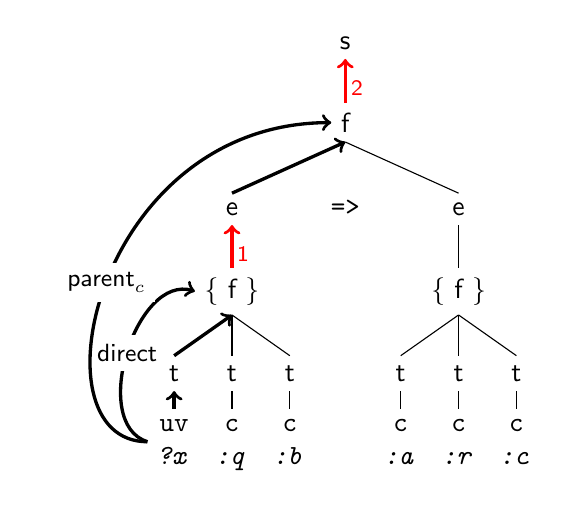
\begin{tikzpicture}
\tikzset{every tree node/.style={align=center,anchor=base}}[sibling distance=150pt]
\Tree [.s \edge[very thick, red,  <-]; [.\node(y){f}; %$\ldots$ 
\edge[very thick,  <-]; 
	[.\node(c){e}; \edge[very thick,  red, <-]; [.\node(a){\{ f \}};   
	               \edge[very thick, <-]; 
	                   [.t \edge[very thick,  <-];  [.\node(x){\texttt{uv}\\{\textit{\texttt{?x}}}}; ] ] 
	                   [.t [.\texttt{c}\\{\textit{\texttt{:q}}} ] ] 
	                   [.t [.\texttt{c}\\{\textit{\texttt{:b}}}   ]  ] ] ]
	 \edge[draw=none];  [.\texttt{=>} ] 
	[.e [.{\{ f \}} [.t [.\texttt{c}\\{\textit{\texttt{:a}}} ] ] [.t [.\texttt{c}\\{\textit{\texttt{:r}}} ] ] [.t [.\texttt{c}\\{\textit{\texttt{:c}}}  ]  ] ] ]
] ]
% \draw[very thick, ->] (x.west)  to  [bend left=90] node [midway,fill=white] {\small{parent}} (y.west);
  \draw[very thick, ->] (x.west) to  [bend left=90] node [midway,fill=white] {\small{direct}} (a.west);
  \draw[very thick, ->] (x.west)..controls +(west:1.5) and +(west:3).. node [midway,fill=white] {\small{$\text{parent}_c$}} (y.west);
   \node[red] (aa) at (-1.3,-2.6) {\footnotesize{1}};
     \node[red] (aaa) at (0.15,-0.5) {\footnotesize{2}};
\end{tikzpicture}\normalsize
\end{center}
\caption{Direct and $\text{parent}_c$ formula. 
% When going through the nodes of the syntax tree from the bottom to the top, the \emph{direct formula} of a component
% \emph{parent formula} of a terminal's direct formula  is
% the formula associated with second node \texttt{f} such that \texttt{f} is a direct child of either an expression \texttt{e}  or the start symbol~\texttt{s}.    
\label{par} }
\end{figure}

To illustrate the idea behind that, we 
%
take  a closer look at one of the concepts used in the informal definitions of \nthree's quantification: %on a concept which is crucial for quantification in \nthree, the concept of parent formulas. %the quantification examples seen so far:
according to the \wwwc team submission~\cite{Notation3} existential variables are quantified on their \emph{direct formula} (Section~\ref{existentials}) and 
universal variables are quantified on their \emph{parent formula} (Section~\ref{universals}). % which therefore need to be identified by a translation mechanism.
%Thus, in order to do a translation from \nthree into core logic, we need to find these
%formulas.
%
%The syntax tree can the concept of 
%To find these two kinds of formulas we can use the syntax tree. %\emph{direct formula} and \emph{parent formula}. 
% which is closely related 
% to quantification in \nthree.
% the behaviour of \nthree's implicit 
% universal quantification as stated in the \wwwc team submission.
%
%
\label{parentformula}
%As discussed in Section~\ref{universals}, implicit universal variables are quantified 
%on the \emph{parent formula} of the formula they \emph{directly occur in}.
Informally 
such a \emph{direct formula} $f$ of a term $t$ is the next formula surrounded by curly brackets \{ \} that contains $t$, or, if such a formula does not exist, 
the top formula. 
In EYE's interpretation, the \emph{parent formula} is now the top formula (concept $\textit{parent}_e$). 
For Cwm, the \emph{parent formula} $g$ of $f$ is the next higher formula surrounded by curly brackets, ie the direct formula of $\{f\}$ ($\textit{parent}_c$). %is a direct component. 
%where \emph{direct} means that  $\{f\}$ is not nested in other \{\}-constructs. 
%
Being the top formula, the $\emph{parent}_e$ \emph{formula} is easy to find. For the \emph{direct formula} and the $\emph{parent}_c$ \emph{formula} we use the syntax tree:
The difference between a simple formula $f$ and a formula in brackets $\{f\}$ is in the grammar point of view the difference between
a \emph{formula} \texttt{f} and a \emph{formula expression}~\texttt{e}.
If we want to find the direct formula of a component and its $\text{parent}_c$, we can go through the syntax tree from the bottom to the top.  
The \emph{direct formula} is then the first formula on that path which is a direct child of either an expression \texttt{e}  or the start symbol~\texttt{s}. 
%ie the 
%first occurrence of a production rule of the form
%$X_0 ::= X_1\ldots X_n$ where $X_0\in \{\texttt{e}, \texttt{s}\}$ and $X_i=\texttt{f}$ for one $i$ with $1\leq i \leq n$.
The $\emph{parent}_c$ \emph{formula} is the second such formula.\footnote{Note that universals on top level like for example in the formula ``\texttt{?x :p :o.}`` 
do not have a $\text{parent}_c$. 
We assume here, that these formulas are also quantified on top level. This differs from Cwm which does not support universal quantification on top level.}
%
%
 %Here and in the remainder of this paper we use italic letters to write terminal symbols.
%The parent formula of a universal variable is the second formula (\texttt{f}) we  encounter
%when going up a syntax tree from the node containing the universal to the root. 
%
We illustrate this in Figure~\ref{par} on the syntax tree of the formula:
\begin{equation}
 \texttt{\{?x :q :b\} => \{:a :r :c\}.}\label{for}
\end{equation}
% If we go up the syntax tree from the terminal node \texttt{?x} to the top, we encounter as first formula expression  \texttt{\{?x :q :b.\}}, the formula 
% \texttt{?x :q :b.} is the parent of \texttt{?x}. If we go higher
The direct formula of the terminal node \texttt{?x} is the formula $\texttt{?x :q :b.}$, the
$\text{parent}_c$ formula is the 
top formula. This $\text{parent}_c$ formula carries the universal quantifier for the variable.
 The formula means according to the \wwwc team submission:
%Thus, the formula means a:
\begin{equation}
\forall \texttt{x. <x q b>}\rightarrow  \texttt{<a r c>.}
 \tag{\ref{for}'}
\end{equation}
Attribute grammars provide a formalism to describe the above process of \emph{going through the syntax tree} in a more precise way. 



\subsection{Attribute Grammars}\label{ag}
\begin{figure}
\begin{tabular}{llclcl}
\hline
\multicolumn{3}{l}{Grammar}&\multicolumn{3}{l}{Synthesized attribute \textit{ds}}\\
%Syntax: &&\\
%&&\\
\hline
\texttt{s ::=}& \texttt{n}&&\texttt{s}.\textit{ds}&$\leftarrow$ & \texttt{n}.\textit{ds}\\
%& \texttt{n}& number\\
 %      &\\
\texttt{n ::= } & %&    \hspace{0.2\textwidth}           numbers:\\  
      \texttt{d} &&  \texttt{n}.\textit{ds} &$\leftarrow$ & %&    \hspace{0.2\textwidth}           numbers:\\  
      \texttt{d}%.\textit{ds}  
      \\%&                digit\\
    &  $\texttt{n}_1 \texttt{n}_2$ &&& $\leftarrow$ & $\texttt{n}_1.\textit{ds} +\texttt{n}_2.\textit{ds}$\\
%\texttt{d ::=}& $i$ with $i\in \{0,1,2,3,4,5,6,7,8,9\}$   \\ 
%\texttt{d ::=}&  \\   
\hline
\end{tabular}
\caption{Context-free grammar producing integers of arbitrary length (left) and definition of the attribute \textit{ds} which composes the digit sum (right). \label{simplegrammar}}
\end{figure}
In this section we give an introduction to attribute grammars~\cite{attributegrammar,ag2}. 
Attribute grammars are defined on top of context-free grammars like the one given above and extend this concept by so-called \emph{attributes}. 
Such attributes 
are defined on the nodes of the syntax tree 
 and can take values.
 These values can depend on other attribute values of the node itself and either its descendent nodes in the syntax tree -- in this case the attribute is called
 \emph{synthesized} -- or 
% they can depend on the node's attributes and 
on the attribute values of the parent node -- in this case it is called \emph{inherited}.
%This formalism is then applied in the following sections to solve, among others, the 
%problem described above.
The definitions used follow the notation of Paakki~\cite{Paakki}.



\subsubsection{Example}
%Before further working with this grammar,
%we use an easier context free grammar to illustrate the idea of attribute grammars. Consider the following context free grammar in  which can be used to generate an integer:
Before providing a formal definition, we illustrate the idea of attribute grammars on a simpler example than the grammar provided above. 
Consider the context-free grammar displayed on the left side of Figure~\ref{simplegrammar}. 
If \texttt{d} can take any value of the alphabet $\mathcal{A}=\{1,2,3,4,5,6,7,8,9,0\}$, %(as a rule $\texttt{d ::= <}\textit{alphabet symbol}{>}$), 
this 
grammar produces integers of arbitrary length.
%
%
%  \begin{figure}
% \begin{tabular}{lcl}
% %Syntax: &&\\
% %&&\\
% \hline
% \texttt{s}.\textit{ds}&$\leftarrow$ & \texttt{n}.\textit{ds}\\
% %& \texttt{n}& number\\
% \texttt{n}.\textit{ds} &$\leftarrow$ & %&    \hspace{0.2\textwidth}           numbers:\\  
%       \texttt{d}  \\%&                digit\\
%     & $\leftarrow$ & \texttt{n}.\textit{ds} +\texttt{n}.\textit{ds}\\
% %\texttt{d}.\textit{ds}&$\leftarrow$ & $i$\\ 
% %\texttt{d ::=}&  \\   
% \hline
% \end{tabular}
% \caption{Rules for the attribute \textit{ds} which produces the digit sum for integers generated by the grammar in Figure~\ref{simplegrammar}. \label{attributeds}}
% \end{figure}
%This grammar can be used to generate an integer of arbitrary length. 
%
A possible\footnote{Note that there are several options to form a tree for 9487, attribute \textit{ds} also computes the digit sum if one of these is chosen.} syntax tree for 9487
is displayed in Figure~\ref{simpletree}. % is displayed in Figure~\ref{simpletree}.
%
\begin{figure}
\begin{center}
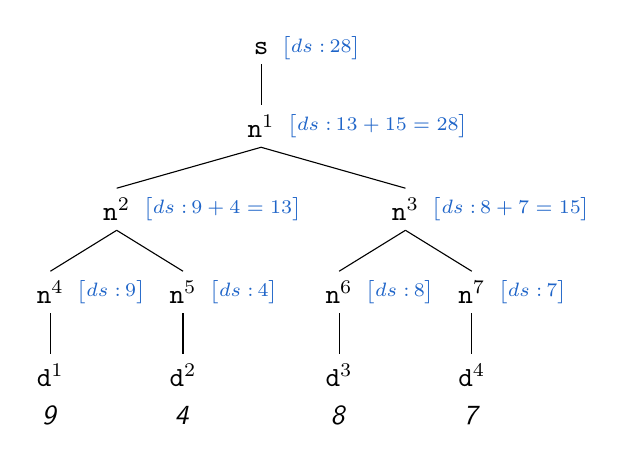
\begin{tikzpicture}
\tikzset{every tree node/.style={align=center,anchor=base}}[sibling distance=300pt]
\Tree [.\node[label={right:\hspace{-0.2cm}\trm{ds:&\hspace{-0.3cm}28}}]{\texttt{s}}; [.\node[label={right:\hspace{-0.2cm}\trm{ds:&\hspace{-0.3cm}13+15=28}}]{$\texttt{n}^1$};
[.\node[label={right:\hspace{-0.2cm}\trm{ds:&\hspace{-0.3cm}9+4=13}}]{$\texttt{n}^2$}; [.\node[label={right:\hspace{-0.2cm}\trm{ds:&\hspace{-0.3cm}9}}]{$\texttt{n}^4$}; 
[.\node[label={below:\emph{9}}]{$\texttt{d}^1$}; ] ] 
[.\node[label={right:\hspace{-0.2cm}\trm{ds:&\hspace{-0.3cm}4}}]{$\texttt{n}^5$}; [.\node[label=below:\emph{4}]{$\texttt{d}^2$}; ] ] ] 
[.\node[label={right:\hspace{-0.2cm}\trm{ds:&\hspace{-0.3cm}8+7=15}}]{$\texttt{n}^3$}; [.\node[label={right:\hspace{-0.2cm}\trm{ds:&\hspace{-0.3cm}8}}]{$\texttt{n}^6$}; 
[.\node[label={below:\emph{8}}]{$\texttt{d}^3$}; ] ] 
[.\node[label={right:\hspace{-0.2cm}\trm{ds:&\hspace{-0.3cm}7}}]{$\texttt{n}^7$}; [.\node[label={below:\emph{7}}]{$\texttt{d}^4$}; ] ] ] ]
]
% \node (b) at (-1.9, -4.1) {} ;
% \node (a) at (-1.9, -3.1) {} ;
% \draw[ugentblue, semithick, ->] (b) to (a);
\end{tikzpicture}
\end{center}
\caption{Syntax tree for 9487 produced by the grammar in Figure~\ref{simplegrammar} 
with attribute values for \emph{ds} (in \color{ugentblue}{\emph{blue}}\color{black}).\label{simpletree}}
\end{figure}
To ease the following discussion, the tree nodes of the same kind are numbered.

If we now want to get the digit sum of an integer produced by that grammar, we can go through the syntax tree from the bottom to the top:
from the nodes resulting in a digit, 
we store that digit. For every node higher in the syntax tree, we take the values of its children and sum them up to a new value. 
Then the values of the start node is the digit sum of 
the integer. 

To formalise this process %of passing information from the bottom of a syntax tree to the top, 
we define the synthesized attribute $\operatorname{\textit{ds}}$. % for all nodes of the syntax tree.
This attribute takes values on each node and these values depend on the production rules of the grammar. 
For each production rule, we define an \emph{attribute rule}.
% For every node $N$ on which an attribute is defined, there are now rules which determine \emph{attribute values} for this node, the \emph{attribute rules}.
% These rules depend on the production rules $X_0 \texttt{ ::= } X_1\ldots X_n$ of the grammar. They can either depend on the rules which have an occurrence of the node on the 
% \emph{right}
% side of 
% the production rule, ie the rules of the form $X_0 \texttt{ ::= } X_1\ldots N \ldots X_n$---in this case they are called \emph{inherited}---%
% or they can depend of the production rules which have the node at the \emph{left} side of the production rule, ie on rules of the form $N \texttt{ ::= } X_1\ldots X_n$---%
% in this case they are called \emph{synthesized}.
% Inherited attributes pass information downwards in the syntax tree, synthesised attributes pass it upwards.
% Since we want the latter, we define our attribute \textit{ds} to be synthesized.
%
% ---in this case they pass information from the top of the syntax tree downwards and are called \emph{inherited}---%
% or they can depend on the rules which have the node on the left hand side---in this case they pass information upwards in the syntax tree and are called \emph{synthesized}. 
% %
%This means that for every node which occurs in a grammar rule there must be a value assigned, the \emph{attribute value}.
%For every node we want to collect in this attribute the digit sum of the number occurring under it.
% for all nodes occurring in the grammar rules.
%In order to pass information from the bottom to the top of the syntax tree as described above, this attribute needs to be \emph{synthesized}.
%Attributes take values for all the nodes they are defined on. %, for a node \texttt{n} and an attribute $a$ we denote that value by $\texttt{n}.a$. 
%These values are determined by so-called \emph{attribute rules}. These are rules which depend on the production rules of the syntax. 
% They can either follow the direction of the 
% production rule---ie define the attribute values of the elements in the body of the production rule based on the attribute values of its head---these are the \emph{inherited} attributes; 
% or they can go in the opposite direction of the production rule---ie define the attribute value of the node in the head of the production rules taking into 
% account the attribute values 
% of the nodes in the body of the rule---these are the \emph{synthesized} attributes. For the process we want to model, we need \textit{ds} to be synthesized since we want to go from the bottom
%to the top of the tree. % ie in the opposite direction of the production rules.
%For our current purpose we need an attribute of the latter kind and let \textit{ds} therefore be synthesized.  
%As our attribute is defined on all nodes, we need to fix one attribute rule for each production rule of the grammar. 
These rules are displayed at the right side
of Figure~\ref{simplegrammar}. 
% Additionally we define that the value $\texttt{d}.\textit{ds}$ is the value of the alphabet symbol connected to \texttt{d} (more formally, we have the grammar 
% rule $\texttt{d ::= <}\textit{alphabet symbol}{>}$ and the attribute rule $\texttt{d}.\textit{ds}\lefttarrow \texttt{<}\textit{alphabet symbol}{>}$).
We denote the attribute value for a node \texttt{n} by \texttt{n}.\textit{ds}. When we use a node resulting in an alphabet symbol of the grammar (in our example \texttt{d}) in an attribute rule,
that symbol refers its alphabet symbol.
Going through the syntax tree from the bottom to the top, we get for 
node $\texttt{n}^4$
%We apply the rules on the syntax tree above. The four terminal nodes have the values:
% $
%  \texttt{d}^1.\textit{ds}=9%;\quad \texttt{d}^2.\textit{ds}= 4;\quad \texttt{d}^3.\textit{ds}= 8;\quad \texttt{d}^4.\textit{ds} = 7
% $
by attribute rule $\texttt{n}.\textit{ds} \leftarrow \texttt{d}$ the value %we get for the nodes $\texttt{n}^4, \texttt{n}^5, \texttt{n}^6$ and $\texttt{n}^7$:
%\[
 $\texttt{n}^4.\textit{ds}=9$. The same rule is used to determine $\texttt{n}^5.\textit{ds}$ to $\texttt{n}^7.\textit{ds}$
 whose values are displayed in Figure~\ref{simpletree}.
%  This is the value 
% of the terminal symbol $\texttt{d}^1$ (9 in this case) upwards to the next node.  
%;\quad \texttt{n}^5.\textit{ds}\leftarrow 4;\quad \texttt{n}^6.\textit{ds}\leftarrow 8;\quad \texttt{n}^7.\textit{ds}\leftarrow 7
%\]
On the next higher level, the attribute value of each node is composed by taking the sum of the attribute values of the direct descendants. This is done by the 
rule $\texttt{n}.\textit{ds}\leftarrow \texttt{n}_1.\textit{ds}+\texttt{n}_2.\textit{ds} $. % bring for the nodes $\texttt{n}^2$ and $\texttt{n}^3$:
We get
 $\texttt{n}^2.\textit{ds}=13$ and
 $\texttt{n}^3.\textit{ds}=15$.
The same rule computes one level higher for $\texttt{n}^1$ the value
$
  \texttt{n}^1.\textit{ds}=28
$
which is then passed to the start node \texttt{s} by the rule $\texttt{s}.\textit{ds}\leftarrow \texttt{n}.\textit{ds}$.
And 28 is indeed the digit sum of 9487.


\subsubsection{Terminology}
% \begin{definition}
% Let  $G=\langle N, \mathcal{A}, P, S\rangle$ be a context free grammar.
% \begin{itemize}
%  \item For each symbol $X\in N\cup \mathcal{A}$ there exists a finite set $A(X)=I(X)\cup S(X)$ of \emph{attributes} with $I(X)\cap S(X) = \emptyset$. We call the set $I(X)$
%  the set of \emph{inherited} attributes and the set $S(X)$ the set of \emph{synthesized} attributes.
%  \item For each left side occurrence $X_0.a$ of a synthesized attribute $a\in S(X)$ in a production rule $p: X_0 \texttt{ ::= } X_1\ldots X_n$ there exists an \emph{attribution rule}
%  \[
%   X.a \leftarrow f(y_1,\ldots, y_k)
%  \]
% where $f$ is a function and $y_i\in A(X_0)\cup A(X_1)\cup\ldots\cup A(X_n)$ for all $1\leq i \leq k$. 
%  \item For each right side occurrence $X_i.a$, $1\leq i \leq n$ of an inherited attribute $a\in I(X)$ in a production rule $p: X_0 \texttt{ ::= } X_1\ldots X_n$ 
%  there exists an \emph{attribution rule}
%  \[
%   X_i.a \leftarrow f(y_1,\ldots, y_k)
%  \]
% where $f$ is a function and $y_i\in A(X_0)\cup A(X_1)\cup\ldots\cup A(X_n)$ for all $1\leq i \leq k$. 
% \end{itemize}
% 
% \end{definition}
%Having seen a concrete example, 
After our example, we now provide a more formal introduction to attribute grammars and fix the terminology we use. 
%
Attribute grammars are defined on top of 
context free grammars
 $G=\langle  N, \mathcal{A}, P, S\rangle$, with $N$ the set of non-terminal symbols,  $\mathcal{A}$ the alphabet or set of terminal symbols, 
$P$ the set of production rules and $S\in N$ a start symbol. 
The set $P$ for the context-free grammar above is displayed in Figure~\ref{simplegrammar}.
This figure also contains all non terminal symbols $N$.
%The alphabet is defined separately and a connection to the alphabet is given by the rule $\texttt{d :: <}\textit{digitsymbol}{>}$.  
The start symbols is \texttt{s}.

For each non-terminal symbol $X\in N$  of the grammar we now define
 a set of attributes $A(X)$. %In our example above, this set of attribute has been for every node $A(X)=\{\textit{ds}\}$.
%
%These attributes are used to pass information through the syntax tree.
%To express that $a\in X$ we use the notation $X.a$.
Each of these attributes either belongs to the set of \emph{inherited} attributes $I(X)$, or to the set of \emph{synthesized} attributes $S(X)$.
%Synthesized attributes are used to pass information from the bottom of a syntax tree to the top like in the example of the previous section, 
%inherited attributes are used for the opposite direction, from the top of a syntax tree to the bottom. 
We assume these two sets of attributes to be disjoint. % $A(X)=I(X)\dot\cup S(X)$.
In our example above we have for each node $X$: $I(X)=\emptyset$, $S(X)=\{\textit{ds}\}$, and $A(X)=\emptyset\cup\{\textit{ds}\}=\{\textit{ds}\}$.
%

To take information, the attributes have assigned values which depend on the production rules they occur in.
%
\begin{definition}[Attribute Occurrence]
Let $G=\langle N, \mathcal{A}, P, S\rangle$ be a context-free grammar and $A:=\bigcup_{X\in N} A(X)$ a set of attributes defined on $N$.
Let $p\in P$
%This assignment depends on the production rules where $X$ occurs in. A rule
be a production rule of the form \[X_0 ::= X_1 \cdots X_n \text{ with } n\geq 1,
\]
\begin{itemize}
\item We say that $p$ has
an \emph{attribute occurrence} $X_i.a$ for the attribute $a$ if $a \in A(X_i)$ for some $i$ with $0\leq i \leq n$.
%\rv{exactly one?}
\item We say that $p$ has a \emph{left-side occurrence}  $X_0.a$ of the attribute $a$, if $a\in A(X_0)$.  
\item We say that $p$ has a \emph{right-side occurrence}  $X_k.a$ of the attribute $a$, if $a\in A(X_k)$ for some $k$ with $1 \leq k \leq n$.
%\rv{exactly one?}
\end{itemize}
\end{definition} 

If we consider another attribute for the grammar in Figure~\ref{simplegrammar}, which is defined only for the node \texttt{d}, the attribute \textit{at},
then the rule
\[
 \texttt{n ::= d} 
\]
has a \emph{right-side occurrence} $\texttt{d}.\textit{at}$ of the attribute \textit{at} while the rule
\[
 \texttt{n ::= n}_1 \texttt{n}_2
\]
does not have any occurrence of \textit{at}.

These occurrences $X_i.a$ now take values, so-called \emph{attribute values}, which are defined by %of a syntezised attribute $X_0.a$ and each occurence of an inherited attribute $X_i.a$, $1\leq i \leq n$, 
 \emph{attribute rules}. These have the form % of the form
\[X_i.a \leftarrow f(y_1\ldots y_n)\]
where $f$ is a function and $y_1\ldots y_n$ are other attribute values. 
An example from above for such an attribute rule is 
\[\texttt{n}.\textit{ds}\leftarrow \texttt{n}_1.\textit{ds}+\texttt{n}_2.\textit{ds} \]
which determines the first occurrence \texttt{n}.\textit{ds} of the attribute \textit{ds} in the production rule
\[
 \texttt{n ::= n}_1 \texttt{n}_2
\]
We denote the set of all
attribute rules for a production rule $p\in P$ by $R(p)$. 
Which exact attribute values can be taken into account when calculating a new attribute value  depends on the kind of attribute:
\begin{definition}[Attribute Grammar]
Let $G=\langle N, \mathcal{A}, P, S\rangle$ be a context-free grammar.
For every element $X\in N$ let $A(X)=I(X)\cup S(X)$ be a finite set of attributes with  $I(X)\cap S(X)=\emptyset$. Let $A=\bigcup_{X\in \mathcal{A}\cup N} A(X)$ 
be the set of all these attributes.
Let  $R=\bigcup_{p\in P} R(p)$ be a finite set of attribute rules.
We call \[AG=\langle G, A, R\rangle\] an \emph{Attribute Grammar} 
if for each production rule $p\in P$ of the form $X_0 \texttt{ ::= } X_1\ldots X_n$ the following holds:
\begin{itemize}
\item for each left-side occurrence $X_0.a$ of a synthesised attribute $a\in S(X_0)$
there exists \emph{exactly one} attribute rule $(X_0.a \leftarrow f(y_1,\ldots,y_k))\in R(p)$ where $f$ is a function and $y_i\in A(X_0)\cup \ldots \cup A(X_n)$ for all $1\leq i \leq k$.
\item for each right-side occurrence $X_i.a$, $1\leq i \leq n$, of an inherited attribute  $a\in I(X_i)$
there exists \emph{exactly one} attribute rule %of the form
$(X_i.a \leftarrow f(y_1,\ldots,y_k))\in R(p)$ where $f$ is a function and $y_j\in A(X_0)\cup \ldots \cup A(X_n)$ for all $1\leq j \leq k$.
\end{itemize}
\end{definition}


%In case of \emph{synthesized attributes} the attribution rules depend on the production rules having the attribute occurrence is on the left side of the rule% 
%the value of an attribute occurrence on the \emph{left} side of a production rule
%is determined taking the attribute values of the right side into account
%---just as we have seen above---% 
%in case of an \emph{inherited attribute} the attribution rules depends on the production rules which have an occurrence on the attribute on the \emph{right}
%side of the rule.
%is determined by taking attribute values of the 
%left hand side into account.
% Above we have seen a synthesized attribute, the attribution rules depended on the production rules carrying the attributed symbol on the left side. In our example, 
% the value of attribute \textit{ds} only depended on the attribute value of \textit{ds} on other nodes. 
% The values can also depend on values of other attributes,
% %These values do not need to be from the same attribute. 
% Note that the attribute value does not only need to depend on  occurrences of the same attribute on different nodes, it could also depend on other values.
% If we for example define our attribute \textit{at} on the node \texttt{d} from above as inherited, a possible attribute rule 
% for the occurrence of the attribute in the rule \texttt{n ::= d} could be:
% \[
%  \texttt{d}.\textit{at} \leftarrow \texttt{n}.\textit{ds}+5
% \]
%or any other value which only depends on attribute values of \texttt{n}.

% Note that the definition states that \emph{inherited} attributes are defined on attribute occurence
% of the right hand side of a rule and \emph{synthesized} attributes are output of the left hand side.
In terms of a syntax tree generated by the grammar synthesized and inherited attributes have exactly the properties mentioned above:  
inherited attributes pass information \emph{down} in the syntax tree, synthesized attributes pass information \emph{upwards}.
We assume the values of synthesized attributes defined on terminal symbols to be defined externally. The start symbol cannot take an inherited attribute.\footnote{The attentive
reader might have noticed another difference in the structure of the context-free grammar of the core logic (Figure~\ref{syntax}) and the syntax of \nthree (Figure~\ref{N3S}):
the latter has an extra start symbol. The reason for this is rather technical: the attribute grammar we define in the following sections makes use of inherited attributes
defined on the symbol \texttt{f}. Such attributes cannot be defined on a start symbol.
} 


\subsection{Definition of an  Attribute Grammar}
\begin{table}
\begin{tabular}{llll}
\hline
name & type %\hspace{0.5cm}
& defined for &purpose \\
 \hline
 $\eq$ & syn  & $ N$& existentials\\
 \\
 $v_1$ & syn &$ N$& universals in Cwm \\
 $v_2$ & syn &$ N$ & universals in Cwm\\
 $s$ & inh &$\{\texttt{f}, \texttt{t},\texttt{e}, \texttt{k}\}$& universals in Cwm \\
  $q$ & inh &$\{\texttt{f}\}$& universals in Cwm \\
  \\
  $u$ & syn &$ N$& universals in EYE \\
  \\
  $m_c$ & syn  &$ N$& translation Cwm\\
  $m_e$ &syn &$ N$& translation EYE \\
  \hline
\end{tabular}
\caption{Overview of all attributes defined in the \nthree-attribute grammar. The type can be \emph{syn} for synthesized or \emph{inh} for inherited. \label{attributes}}
\end{table}

After the definition of attribute grammars in the previous section, 
%Having introduced attribute grammars in the previous section, 
we now apply this concept to 
formalise the different interpretations of implicit quantification for \nthreelogic. 
The context-free grammar of \nthree is given in Figure~\ref{N3S} which also contains all symbols of~$N$. The alphabet is given in Definition~\ref{alphabet}. 
The start symbol is~\texttt{s}.

On top of this grammar we now define an attribute grammar in order to be able to produce the two different translations %
of an \nthree formula in core logic, one according to Cwm and the team submission and the other according to EYE.
As a first step we define the sets of attributes for all symbols $X\in N$.
% For all $X\in (N\cup \mathcal{X})\setminus \{\texttt{f}, \texttt{s}\}$ these are 
% \[
%  S(X)=\{\eq, v_1, v_2, u, m_c, m_e\} \text{ and } I(X)=\{s\}
% \]
% For \texttt{s} these are 
% \[
%  S(\texttt{s})=\{\eq, v_1, v_2, u, m_c, m_e\} \text{ and } I(\texttt{s})=\emptyset
% \]
% For \texttt{f} these are
% \[
%  S(\texttt{f})=\{\eq, v_1, v_2, u, m_c, m_e\} \text{ and } I(\texttt{f})=\{s, q\}
% \]
These are displayed in Table~\ref{attributes}. 
For each of these attributes we also indicated the purpose or context they are used for. This context can be grouped in four parts:  the collection of the variables which are existentially 
quantified under a (sub-)formula (1), the collection
of the universal variables quantified under a (sub-)formula -- once for Cwm (2) and once for EYE (3) -- and attributes to construct the concrete 
expression in core logic which is the translation of the \nthree 
formula dependent on the reasoner (4).
In the following we will go through these four groups one by one, explain the need for the different attributes and provide their definition. We start with attribute $\eq$, which is used for existential scoping. 
%We will explain and define these attributes in this and the following sections.
%We begin with the attribute 
%for existential variables.

\subsubsection{Existentials}\label{exsec}
% tree without labels
% \begin{figure}
% \begin{center}
% \begin{tikzpicture}
% \tikzset{every tree node/.style={align=center}}[sibling distance=140pt]
% \Tree [.\texttt{s} [.\node{$\texttt{f}^1$}; %$\ldots$
% 	[.\node{$\texttt{t}^1$}; [.\node[label={below:\textit{\texttt{\_:x}}}]{$\texttt{ex}^1$}; ] ]          
% 	    % [.t [.\node(x)[label={right: \footnotesize{$v_1=\{\texttt{\textit{?x}}\}$}}]{\texttt{uv}\\{\textit{\texttt{?x}}}}; ] ]  [.t [.\texttt{c}\\{\textit{\texttt{:q}}} ] ] [.t [.\texttt{c}\\{\textit{\texttt{:b}}}   ]  ] ] ]
% 	[.$\texttt{t}^2$ [.\node[label={below:\textit{\texttt{:s}}}]{$\texttt{c}^1$}; ] ] 
% 	[.$\texttt{t}^3$ [.\node(e){\texttt{e}}; [.\node(a){\{$\texttt{f}^2$\}}; 
% 	    [.\node{$\texttt{t}^4$}; [.\node(z)[label={below:\textit{\texttt{\_:y}}}]{$\texttt{ex}^2$}; ] ] 
% 	    [.$\texttt{t}^5$ [.\node[label={below:\textit{\texttt{:k}}}]{$\texttt{c}^2$}; ] ] 
% 	    [.$\texttt{t}^6$ [.\node[label={below:\textit{\texttt{:a}}}]{$\texttt{c}^3$};  ]  ] ] ]
% ] ] ]
% 
%  %\draw[semithick, ->] (z) to  [bend left=90] node [midway,fill=white] {direct} (a);
%  %\draw[semithik, ->] (z) to [bend left=80]  node [midway,fill=white] {$\operatorname{uv}_2=\{\texttt{?x}\}$} (a);
%  %\draw[semithik, ->] (a) to [bend left=80]  node [midway,fill=white] {$\operatorname{sc}=\{\texttt{?x}\}$} (b);
% \end{tikzpicture}\normalsize
% \end{center}
% \caption{Syntax tree for Formula~\ref{eq99}. \label{extreesimple} }
% \end{figure}

% \begin{figure}
% \begin{center}
% \begin{tikzpicture}[
% every tree node/.style={align=center},
% %sibling distance=1cm,
% %level distance =100pt,
% level 2/.style={level distance=40pt},
% level 5/.style={level distance=40pt}
% ]
% \Tree [.\node[label={right:\tr{$\texttt{s}.\eq=\emptyset$}}]{\texttt{s}}; [.\node[label={right:\tr{$\texttt{f}^1.\eq=\{\texttt{\_:x}\}$}}]{$\texttt{f}^1$}; %$\ldots$
% 	[.\node[label={right:\tr{$\texttt{t}^1.\eq=\{\texttt{\_:x}\}$}}]{$\texttt{t}^1$}; [.\node[label={below:\textit{\texttt{\_:x}}}]{$\texttt{ex}^1$}; ] ]          
% 	    % [.t [.\node(x)[label={right: \footnotesize{$v_1=\{\texttt{\textit{?x}}\}$}}]{\texttt{uv}\\{\textit{\texttt{?x}}}}; ] ]  [.t [.\texttt{c}\\{\textit{\texttt{:q}}} ] ] [.t [.\texttt{c}\\{\textit{\texttt{:b}}}   ]  ] ] ]
% 	[.\node[label={right:\tr{$\texttt{t}^2.\eq=\emptyset$}}]{$\texttt{t}^2$}; [.\node[ label={below:\textit{\texttt{:s}}}]{$\texttt{c}^1$}; ] ] 
% 	[.\node[label={right:\tr{$\texttt{t}^3.\eq=\emptyset$}}]{$\texttt{t}^3$}; [.\node(e)[label={right:\tr{$\texttt{e}.\eq=\emptyset$}}]{\texttt{e}}; [.\node(a)[label={right:\tr{$\texttt{f}^2.\eq=\{\texttt{\_:y}\}$}}]{\{$\texttt{f}^2$\}}; 
% 	    [.\node[label={right:\tr{$\texttt{t}^4.\eq=\{\texttt{\_:y}\}$}}]{$\texttt{t}^4$}; [.\node(z)[label={below:\textit{\texttt{\_:y}}}]{$\texttt{ex}^2$}; ] ] 
% 	    [.\node[label={right:\tr{$\texttt{t}^5.\eq=\emptyset$}}]{$\texttt{t}^5$}; [.\node[label={below:\textit{\texttt{:k}}}]{$\texttt{c}^2$}; ] ] 
% 	    [.\node[label={right:\tr{$\texttt{t}^6.\eq=\emptyset$}}]{$\texttt{t}^6$}; [.\node[label={below:\textit{\texttt{:a}}}]{$\texttt{c}^3$};  ]  ] ] ]
% ] ] ]
% \end{tikzpicture}\normalsize
% \end{center}
% \caption{Syntax tree for Formula~\ref{eq99} with values for the attribute $\eq$ (in \tr{blue}). \label{extreesimple} }
% \end{figure}

% tree with long names
% \begin{figure}
% \begin{center}
% \begin{tikzpicture}[
% every tree node/.style={align=center},
% sibling distance=-0.1cm,
% %level distance =100pt,
% level 2/.style={level distance=40pt},
% level 5/.style={level distance=40pt}
% ]
% \linespread{0.5}
% \Tree [.\node[label={right:\tr{$\texttt{s}.\eq=\emptyset$}}]{\texttt{s}}; [.\node[label={right:\tr{$\texttt{f}^1.\eq=\{\texttt{\_:x}\}$}}]{$\texttt{f}^1$}; %$\ldots$
% 	[.\node[label={[align=right]right:{\vspace{3cm}\tr{$\texttt{t}^1.\eq=\{\texttt{\_:x}\}$}}}]{$\texttt{t}^1$}; [.\node[label={below:\textit{\texttt{\_:x}}}]{$\texttt{ex}^1$}; ] ]          
% 	    % [.t [.\node(x)[label={below: \footnotesize{$v_1=\{\texttt{\textit{?x}}\}$}}]{\texttt{uv}\\{\textit{\texttt{?x}}}}; ] ]  [.t [.\texttt{c}\\{\textit{\texttt{:q}}} ] ] [.t [.\texttt{c}\\{\textit{\texttt{:b}}}   ]  ] ] ]
% 	[.\node[label={[align=left] right:\tr{$\texttt{t}^2.\eq=\emptyset$}\hspace{-1cm}}]{$\texttt{t}^2$}; [.\node[ label={below:\textit{\texttt{:s}}}]{$\texttt{c}^1$}; ] ] 
% 	[.\node[label={right:\tr{$\texttt{t}^3.\eq=\emptyset$}}]{$\texttt{t}^3$}; [.\node(e)[label={right:\tr{$\texttt{e}.\eq=\emptyset$}}]{\texttt{e}}; [.\node(a)[label={left:\tr{$\texttt{f}^2.\eq=\{\texttt{\_:y}\}$}}]{\{$\texttt{f}^2$\}}; 
% 	    [.\node[label={[font=\footnotesize, align=center]  left:\hspace{-1.5cm}\tr{$\texttt{t}^4.\eq=\{\texttt{\_:y}\}$}}]{$\texttt{t}^4$}; [.\node(z)[label={below:\textit{\texttt{\_:y}}}]{$\texttt{ex}^2$}; ] ] 
% 	    [.\node[label={[align=right] left:\tr{$\texttt{t}^5.\eq{}={}\emptyset$}\hspace{-0.1cm}}]{$\texttt{t}^5$}; [.\node[label={below:\textit{\texttt{:k}}}]{$\texttt{c}^2$}; ] ] 
% 	    [.\node[label={[align=right] left:\tr{$\texttt{t}^6.\eq=\emptyset$}\hspace{-0.1cm}}]{$\texttt{t}^6$}; [.\node[label={below:\textit{\texttt{:a}}}]{$\texttt{c}^3$};  ]  ] ] ]
% ] ] ]
% \end{tikzpicture}\normalsize
% \end{center}
% \caption{Syntax tree for Formula~\ref{eq99} with values for the attribute $\eq$ (in \tr{blue}). \label{extreesimple} }
% \end{figure}

\begin{figure}
\begin{center}
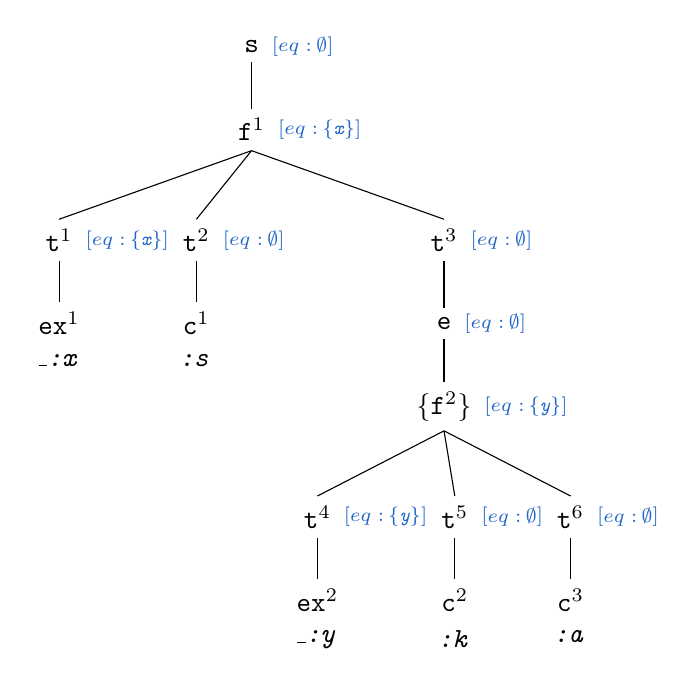
\begin{tikzpicture}[
every tree node/.style={align=center},
sibling distance=-0.1cm,
%level distance =100pt,
level 2/.style={level distance=40pt},
level 5/.style={level distance=40pt}
]
\linespread{0.5}
\Tree [.\node[label={right:\hspace{-0.2cm}\trm{eq:&\hspace{-0.3cm}\emptyset}}]{\texttt{s}}; [.\node[label={right:\hspace{-0.2cm}\trm{eq:&\hspace{-0.3cm}\{\texttt{x}\}}}]{$\texttt{f}^1$}; %$\ldots$
	[.\node[label={right:\hspace{-0.2cm}\trm{eq:&\hspace{-0.3cm}\{\texttt{x}\}}}]{$\texttt{t}^1$}; [.\node[label={below:\textit{\texttt{\_:x}}}]{$\texttt{ex}^1$}; ] ]          
	    % [.t [.\node(x)[label={below: \footnotesize{$v_1=\{\texttt{\textit{?x}}\}$}}]{\texttt{uv}\\{\textit{\texttt{?x}}}}; ] ]  [.t [.\texttt{c}\\{\textit{\texttt{:q}}} ] ] [.t [.\texttt{c}\\{\textit{\texttt{:b}}}   ]  ] ] ]
	[.\node[label={right:\hspace{-0.2cm}\trm{eq:&\hspace{-0.3cm}\emptyset}}]{$\texttt{t}^2$}; [.\node[ label={below:\textit{\texttt{:s}}}]{$\texttt{c}^1$}; ] ] 
	[.\node[label={right:\hspace{-0.2cm}\trm{eq:&\hspace{-0.3cm}\emptyset}}]{$\texttt{t}^3$}; [.\node(e)[label={right:\hspace{-0.2cm}\trm{eq:&\hspace{-0.3cm}\emptyset}}]{\texttt{e}}; 
	 [.\node(a)[label={right:\hspace{-0.2cm}\trm{eq:&\hspace{-0.3cm}\{\texttt{y}\}}}]{\{$\texttt{f}^2$\}}; 
	    [.\node[label={right:\hspace{-0.2cm}\trm{eq:&\hspace{-0.3cm}\{\texttt{y}\}}}]{$\texttt{t}^4$}; [.\node(z)[label={below:\textit{\texttt{\_:y}}}]{$\texttt{ex}^2$}; ] ] 
	    [.\node[label={right:\hspace{-0.2cm}\trm{eq:&\hspace{-0.3cm}\emptyset}}]{$\texttt{t}^5$}; [.\node[label={below:\textit{\texttt{:k}}}]{$\texttt{c}^2$}; ] ] 
	    [.\node[label={right:\hspace{-0.2cm}\trm{eq:&\hspace{-0.3cm}\emptyset}}]{$\texttt{t}^6$}; [.\node[label={below:\textit{\texttt{:a}}}]{$\texttt{c}^3$};  ]  ] ] ]
] ] ]
\end{tikzpicture}\normalsize
\end{center}
\caption{Syntax tree for Formula~\ref{eq99} with values for the attribute $\eq$ (in \tr{blue}). \label{extreesimple} }
\end{figure}

% \begin{figure}
% \begin{tabular}{lll}
% \hline
% \multicolumn{2}{l}{production rule} & attribute rule\\
%   \hline
% %Syntax: &&\\
% %&&\\
% \texttt{s ::=}&\texttt{f}& $\texttt{s}.\eq \leftarrow \texttt{f}.\eq$\\
%        &&\\
% \texttt{f ::= } &  $ \texttt{t}_1 \texttt{t}_2 \texttt{t}_3.$&   $ \texttt{f}.\eq \leftarrow \texttt{t}_1.\eq\cup \texttt{t}_2.\eq\cup \texttt{t}_3.\eq$ \\
%     &  $\texttt{e}_1 \texttt{=>}  \texttt{e}_2.$& $\texttt{f}.\eq \leftarrow \texttt{e}_1.\eq\cup \texttt{e}_2.\eq$ \\
% %    &  \texttt{@forAll :u}     & universal quantification\\
% %    &  \texttt{@forSome :u}     & existential quantification\\
%     & $ \texttt{f}_1 \texttt{f}_2$ &                $\texttt{f}.\eq \leftarrow \texttt{f}_1.\eq\cup \texttt{f}_2.\eq$ \\
% &&\\
% \texttt{t ::=}& \texttt{uv}\hspace{0.07\textwidth} &                $\texttt{t}.\eq \leftarrow\emptyset$\\
%             & \texttt{ex} &               $\texttt{t}.\eq \leftarrow \{\texttt{ex}\}$\\
%       & \texttt{c} &               $\texttt{t}.\eq \leftarrow\emptyset$\\
%  %     & \texttt{l} &                literals\\
%       & \texttt{e} &                $\texttt{t}.\eq \leftarrow\texttt{e}.\eq $\\
%       & \texttt{(k)}& $\texttt{t}.\eq \leftarrow\texttt{k}.\eq$\\
%       & \texttt{()}& $\texttt{t}.\eq \leftarrow\emptyset$\\
%       &&\\
% \texttt{k ::=}& \texttt{t}& $\texttt{k}.\eq \leftarrow\texttt{t}.\eq$\\
% &\texttt{t k} & $\texttt{k}.\eq \leftarrow\texttt{t}.\eq\cup\texttt{k}.\eq$\\
% &&\\
% \texttt{e ::=}&\texttt{\{f\}} &                $\texttt{e}.\eq \leftarrow\emptyset$\\
%        &\texttt{\{\}} &  $\texttt{e}.\eq \leftarrow\emptyset$\\
%        &\texttt{false}       &                $\texttt{e}.\eq \leftarrow\emptyset$\\
%   \hline
% \end{tabular}
% \caption{Attribute rules for the synthesized attribute $\eq$ (right) and their corresponding production rules (left) from the \nthree grammar (Figure~\ref{N3S}).\label{EQ}}
% \end{figure}

As we have seen in Section~\ref{existentials} the scope on an implicitly existentially quantified variable is the \emph{direct} formula it occurs in. 
The concept of a \emph{direct formula} has been further explained above: 
the direct formula is either the next formula in curly brackets surrounding the existential variable, or -- in case such a formula does not exist -- the formula as a whole.
To recall the idea, consider the following formula:\footnote{Note that structure-wise this formula follows the same pattern as Formula~\ref{eq1}. 
The names of constants are only shortened to
make the presentation of the formula easier.}
% Version without underbrace
\begin{equation}
\texttt{\_:x :s \{\_:y :k :a.\}.} \label{eq99}
\end{equation}
% \begin{equation}
% \underbrace{\texttt{\_:x :s }\underbrace{\texttt{\{\_:y :k :a.\}}}_{\text{direct formula of} \texttt{\_:y}}.}_{\text{direct formula of} \texttt{\_:x}} \label{eq99}
% \end{equation}
The direct formula of variable \texttt{\_:y} is the sub-formula \texttt{\_:y :k :a.} The direct formula of \texttt{\_:x} is
the formula as a whole.
Translated into core logic the formula means:
\begin{equation}\tag{\ref{eq99}'}\label{eq99'}
 \exists \texttt{x.x s <}\exists \texttt{y.y k a>.}
\end{equation}


% The direct formula of variable \texttt{\_:y} is the sub-formula \texttt{\_:y :k :a.} and this is also the formula which carries the existential quantifier for the variable. The direct formula of \texttt{\_:x} is
% the formula as a whole and that is also the formula on which this variable is quantified.
% Translated into core logic the formula means:
% \begin{equation}\tag{\ref{eq99}'}\label{eq99'}
%  \exists \texttt{x.x s <}\exists \texttt{y.y k a>.}
% \end{equation}
% In Section~\ref{n3synsec} we also discussed the idea of using the syntax tree 
% As discussed in Section~\ref{n3synsec} we can use the syntax tree to find a variable's direct formula. This syntax tree is displayed in Figure~\ref{extreesimple} 
% and we again numbered the different occurrences of the same node. 
% To find the direct formula of an existential variable we can go up from the terminal 
% node the variable occurs in till the node in which the 
%Attribute $\eq$ is now used to 
%We now want to define an attribute whose value is the set of existential variables which are quantified within the same direct formula as the node carrying the attribute and occur under this particular node.
In Section~\ref{n3synsec} we discussed the idea of using the syntax tree to find the direct formula. 
If we go upwards in the syntax tree from the occurrence of an existential variable to the next higher node \texttt{e} or \texttt{s}, 
the child formula \texttt{f} of that node
is the existential's direct formula which thus carries its quantifier. %As an example consider 
The syntax tree for our example, Formula~\ref{eq99}, is displayed in Figure~\ref{extreesimple}. 
Here node $\texttt{f}^2$ is such a node
for \texttt{\_:y}  and node $\texttt{f}^1$ for \texttt{\_:x}.

Attribute $\eq$ is now used in this context to keep track of all existential variables which need to be quantified.
%In order to construct a translation as
%
%under such a direct formula. 
If we do a direct translation
of the symbols of the alphabet as mentioned at the end of Section~\ref{n3synsec} and add existential quantifiers whenever we encounter a direct formula, 
the attribute carries for each node the set of
existential variables which are free (see Definition~\ref{free}) under that node and need to be bound when new existential quantifiers are added.

%For the node $\texttt{f}_1$
%In such a process (which will be further explained in Section~\ref{all})
%Let's assume that the quantifiers are added by an synthesized attribute which does this addition whenever a step from a formula \texttt{f} 
%to either the node \texttt{e} or \texttt{s}
%is done (we explain this in detail in Section~\ref{all}), then the value of this attribute on the node $\texttt{f}_1$ is:
% At the step which adds the quantifiers to a translated formula (this is explained in Section~\ref{all}) the value of the attribute $\eq$ is used to know which existential 
% variables need to be quantified.
%To add the existential quantifiers in the translation, we can then make use of the value of $\eq$ whenever we reach a direct formula.
% For the language element 
% \[
%  \texttt{x s <}\exists \texttt{y.y k a>.}
% \]
% Here the variable \texttt{x} is free while \texttt{y} is bound. The value of $\eq$ contains exactly this variable \texttt{x} and
% the translating process uses this information to produce the Formula~\ref{eq99'} as attribute value for the start node \texttt{s}.
%In the translation process whose attributes are further explained in Section~\ref{all} this will be the 
% value of the translation when performing the step from the formula to a node \texttt{s} or \texttt{e} the existential quantifiers are added for all the existential
% variables which occur freely under the node. This would here lead to Formula~\ref{eq99'}. 
% 
% 
% 
% is following this idea: 
% 
% in order to be able to construct such a Core Logic translation as provided in Formula~\ref{eq99'}
% %form Formula~\ref{eq99} 
% we 
% need to know which variables are existentially quantified under a direct formula. 
% The synthesized attribute is passing existentially quantified variables
% upwards in the syntax tree till they reach their direct formula. When constructing a translation, these variables 
% get bound on that direct formula. 
% They are irrelevant for higher nodes of the syntax tree and are therefore not passed further.
% 
% 
% 
%  
% 
% 
% To be able to
% then also construct a translation, we do not only need to find the formulas which carry quantifiers, we also need to pass the quantified variables to that direct formula. 
% This is the purpose of the synthesized attribute $\eq$  
% 
% 
% to perform the translation from  Formula~\ref{eq99} to Formula~\ref{eq99'}.
% This syntax tree is displayed in Figure~\ref{extreesimple}.
% using an attribute grammar, we need to pass the information which variables are existentially quantified
% under a direct formula
% from the place where the symbol occurs, ie the bottom of the syntax tree, to
% this formula. This is the purpose of the synthesized attribute $\eq$. 
%From a core logic's point of view the attribute value of every node is the set of free (see Definition~\ref{free}) existential variables occurring under that node.
% For each node the value of the attribute represents the set of variables occurring in its descendent nodes
% which are quantified on the same direct formula the node occurs in. From the translations point of view, 
% for every node which does not represent a direct formula the value of $\eq$
% is the set of existential variables which occur as free variables (see Definition~\ref{free}) under that node.
\begin{figure}
\begin{tabular}{lll}
\hline
\multicolumn{2}{l}{production rule} & attribute rule\\
  \hline
%Syntax: &&\\
%&&\\
\texttt{s ::=}&\texttt{f}& $\texttt{s}.\eq \leftarrow \emptyset$\\
       &&\\
\texttt{f ::= } &  $ \texttt{t}_1 \texttt{t}_2 \texttt{t}_3.$&   $ \texttt{f}.\eq \leftarrow \texttt{t}_1.\eq\cup \texttt{t}_2.\eq\cup \texttt{t}_3.\eq$ \\
    &  $\texttt{e}_1 \texttt{=>}  \texttt{e}_2.$& $\texttt{f}.\eq \leftarrow \texttt{e}_1.\eq\cup \texttt{e}_2.\eq$ \\
%    &  \texttt{@forAll :u}     & universal quantification\\
%    &  \texttt{@forSome :u}     & existential quantification\\
    & $ \texttt{f}_1 \texttt{f}_2$ &                $\texttt{f}.\eq \leftarrow \texttt{f}_1.\eq\cup \texttt{f}_2.\eq$ \\
&&\\
\texttt{t ::=}& \texttt{uv}\hspace{0.07\textwidth} &                $\texttt{t}.\eq \leftarrow\emptyset$\\
            & \texttt{ex} &               $\texttt{t}.\eq \leftarrow \{\texttt{ex}\}$\\
      & \texttt{c} &               $\texttt{t}.\eq \leftarrow\emptyset$\\
 %     & \texttt{l} &                literals\\
      & \texttt{e} &                $\texttt{t}.\eq \leftarrow\texttt{e}.\eq $\\
      & \texttt{(k)}& $\texttt{t}.\eq \leftarrow\texttt{k}.\eq$\\
      & \texttt{()}& $\texttt{t}.\eq \leftarrow\emptyset$\\
      &&\\
\texttt{k ::=}& \texttt{t}& $\texttt{k}.\eq \leftarrow\texttt{t}.\eq$\\
&$\texttt{t k}_1$ & $\texttt{k}.\eq \leftarrow\texttt{t}.\eq\cup\texttt{k}_1.\eq$\\
&&\\
\texttt{e ::=}&\texttt{\{f\}} &                $\texttt{e}.\eq \leftarrow\emptyset$\\
       &\texttt{\{\}} &  $\texttt{e}.\eq \leftarrow\emptyset$\\
       &\texttt{false}       &                $\texttt{e}.\eq \leftarrow\emptyset$\\
  \hline
\end{tabular}
\caption{Attribute rules for the synthesized attribute $\eq$ (right) and their corresponding production rules (left) from the \nthree grammar (Figure~\ref{N3S}).\label{EQ}}
\end{figure}
%
%

Following that idea, we define the attribute rules for $\eq$.
%To better understand this idea, we now define the attribute rules:
As $\eq$ is synthesised % and defined for all nodes of the grammar.
%To formalise the idea above we need to define the attribute rules for $\eq$. As $\eq$ is synthesised and defined on all symbols of the grammar, 
we need to state one attribute rule  for each left-side occurrence of an attribute on a production rule of Figure~\ref{N3S}. 
As the attribute is defined for all nodes, we need one attribute rule for each production rule.
% 
% From the production rules occurring at the bottom of the syntax tree, ie the rules only producing symbols of the alphabet, there is one rule which deserves special attention,
% the production rule (\texttt{t ::= ex}): this rule produces an existential variable which at this point occurs as a free variable since we did not find its direct formula yet. 
% The attibute rule for this production rule ($\texttt{t}.\eq \leftarrow \{\texttt{ex}\}$) collects this existential variable in a sigelton set. 
% For all other rules only resulting in symbols of the alphabet the empty set is assigned by the attribution rule since attribute $\eq$ only collects existentials.
% 
% Most other rules now pass the set of existentials upwards in the syntax tree like for example all rules defined for formulas \texttt{f}. There are two exeptions from this:
% 
% 
% 
These attribute rules are displayed in Figure~\ref{EQ} (right) next to their corresponding production rules (left). 
To illustrate how this attribute works, we added the attribute values for each node to the syntax tree in Figure~\ref{extreesimple}.
We explain these rules by going through the tree %The attribute values for each node of the tree are 
%We 
beginning at the bottom.
%To better understand how the rules work, we compute the attribute values for the nodes of the syntax tree in Figure~\ref{extreesimple}.

The production rule (\texttt{t ::= ex}) results in an existential variable and this variable is not quantified under that node.
%When this rule is applied, there is thus Under the node \texttt{t} whose descendent is produced by this rule, there is thus
%exactly one existential variable occurring freely under that node, the existential \texttt{ex}. 
Therefore, the corresponding attribute rule ($\texttt{t}.\eq \leftarrow \{\texttt{ex}\}$) collects this variable in a singleton set 
(values $\texttt{t}^1.\eq$ and $\texttt{t}^4.\eq$). 
%we have the attribute rule .
%For $\texttt{t}^1$ and $\texttt{t}^4$ we get: %whose rule (\texttt{t~::=~ex}) produces existential variables we get via $\texttt{t}.\eq \leftarrow \{\texttt{ex}\}$:
%\[
% \texttt{t}^1.\eq \leftarrow \{\texttt{ex}\}=\{\texttt{\_:x}\}\quad \text{and} \quad  \texttt{t}^4.\eq \leftarrow\{\texttt{ex}\}= \{\texttt{\_:y}\}
%\]
%Here the attribute value stores the existential variable occurring under the node for which the direct formula has not been found yet. 
The attribute rules for other production rules directly resulting in only symbols of the alphabet do not pass any values since there are
no free existential variables occurring under them. 
For the applications of \texttt{t ::= c} %in our syntax tree we get via 
the attribute rule
%
 $\texttt{t}\leftarrow \emptyset$ assigns the empty set to the nodes $\texttt{t}^2$, $\texttt{t}^5$ and $\texttt{t}^6$.
% \[
%  \texttt{t}^2.\eq \leftarrow \emptyset; \quad  \texttt{t}^5.\eq \leftarrow \emptyset;\quad  \texttt{t}^6.\eq \leftarrow \emptyset
% \]
Most other rules now pass the variables from the descendant nodes up to the parents. 
The attribute value  of a
 formula node \texttt{f} 
is the union of its descendants' values. For $\texttt{f}^2$ that is the set $\{\texttt{\_:y}\}$.
% For the production rule ($\texttt{f ::= t}_1 \texttt{t}_2 \texttt{t}_3$) 
% we have the attribute rule $\texttt{f}.\eq \leftarrow \texttt{t}_1.\eq\cup \texttt{t}_2.\eq \cup \texttt{t}_3.\eq$ and get for $\texttt{f}^2$:
% \[
%  \texttt{f}^2 \leftarrow \texttt{t}^4.\eq\cup \texttt{t}^5.\eq\cup \texttt{t}^6.\eq= \{\texttt{\_:y}\}\cup \emptyset \cup \emptyset = \{\texttt{\_:y}\}
% \]
The only exceptions for this behaviour of passing the variables upwards can be found on the attribute rules for the production rules \texttt{s ::= f} 
and \texttt{e ::= \{f\}}. 
As discussed above, the child formulas \texttt{f} of 
\texttt{e} or \texttt{s} are \emph{direct formulas}. % and can thus carry existential quantifiers. 
All free existential variables occurring 
under such direct formulas get bound on these formulas. The attribute rules for \texttt{s ::= f} 
and \texttt{e ::= \{f\}} thus do  not pass any variables upwards. 
%and assign the empty set as
%attribute value. 
% The attribute rule for $\texttt{f}_2$'s parent now deserves special attention. If the production rule (\texttt{e ::= \{f\}}) is applied, we know that \texttt{f} is a 
% \emph{direct formula}, all free existentially quantified variables occurring under the node \texttt{f} are bound by existential quantifiers on this formula in the translation. 
% The attribute rule does thus not pass any existential variable to the parent node. % and has the form $\texttt{e}\leftarrow \emptyset$. 
The attribute value for node \texttt{e} in our syntax tree is the empty set.
% \[
%  \texttt{e}.\eq\leftarrow \emptyset
% \]
This value is again passed upwards via the attribute rule $\texttt{t}.\eq\leftarrow \texttt{e}.\eq$ % for the production rule (\texttt{t ::= e}):
% \[
% \texttt{t}^3.\eq\leftarrow \texttt{e}.\eq= \emptyset 
% \]
and can the be used to determine the attribute value for $\texttt{f}_1$
which is again the union of all its direct descendants' 
values ($\texttt{f}^2.\eq = \{\texttt{\_:x}\}$).
% , again by applying the rule $\texttt{f}.\eq \leftarrow \texttt{t}_1.\eq\cup \texttt{t}_2.\eq \cup \texttt{t}_3.\eq$:
% \[
%  \texttt{f}^2 \leftarrow \texttt{t}^1.\eq\cup \texttt{t}^2.\eq\cup \texttt{t}^3.\eq= \{\texttt{\_:x}\}\cup \emptyset \cup \emptyset = \{\texttt{\_:x}\}
% \]
This node is again a direct formula, it is the child node of the node \texttt{s}. All existential variables are thus bound on $\texttt{f}^2$, the attribute rule does not pass
existential variables upwards. %We get:
%Similarly to the production rule for a formula expression, the attribute rule for the production rule (\texttt{s ::= f}) 
%does not pass any value since the existential variables are bound on this direct formula, we get:
% \[
%  \texttt{s}\leftarrow \emptyset
% \]
%Having for every attribute the set of existentials occurring as free variables under the node enables 

The attribute value of $\eq$ is always the set of free existential variables occurring under a node. For the formulas $\texttt{f}^1$ 
and $\texttt{f}^2$ these are the sets $\texttt{\{\_:x\}}$ and $\texttt{\{\_:y\}}$, respectively. These are exactly the variables existentially quantified on these formulas as can be seen in 
Formula~\ref{eq99'}.
%Of course it is not enough to simply keep track of the existential variables which are free under a node in the syntax tree. 
%We also need to know which variables are universally quantified under each direct formula. This is the topic of the next sections.

% For the existential nodes we get via $\texttt{ex}.\eq$:
% 
% These nodes carry existential variables whose direct formula is not found yet. 
% The rules for the term nodes \texttt{t} are all used to pass information upwards
% 
% 

% \begin{figure}
% \begin{tabular}{rcl}
%   \hline
% %Syntax: &&\\
% %&&\\
% $\texttt{s}.\eq$ & $\leftarrow$ & $\texttt{f}.\eq$\\
%        &&\\
% $ \texttt{f}.\eq$&$ \leftarrow$ & $\texttt{t}_1.\eq\cup \texttt{t}_2.\eq\cup \texttt{t}_3.\eq$ \\
%  $\texttt{f}.\eq$ &  $\leftarrow$ & $\texttt{e}_1.\eq\cup \texttt{e}_2.\eq$ \\
% %    &  \texttt{@forAll :u}     & universal quantification\\
% %    &  \texttt{@forSome :u}     & existential quantification\\
%               $\texttt{f}.\eq$ & $\leftarrow$ & $\texttt{f}_1.\eq\cup \texttt{f}_2.\eq$ \\
% &&\\
%                 $\texttt{t}.\eq$ & $\leftarrow$ &$\emptyset$\\
%            $\texttt{t}.\eq$& $\leftarrow$ & $ \{\texttt{ex}\}$\\
%              $\texttt{t}.\eq$ &$\leftarrow$ & $ \emptyset$\\
%  %     & \texttt{l} &                literals\\
%               $\texttt{t}.\eq$ & $  \leftarrow$ & $ \texttt{e}.\eq $\\
%   $\texttt{t}.\eq$ & $  \leftarrow$ & $ \texttt{k}.\eq$\\
% $\texttt{t}.\eq$ & $  \leftarrow$ & $ \emptyset$\\
%       &&\\
% $\texttt{k}.\eq $ & $ \leftarrow$ & $ \texttt{t}.\eq$\\
%  $\texttt{k}.\eq $ & $ \leftarrow$ & $ \texttt{t}.\eq\cup\texttt{k}.\eq$\\
% &&\\
%               $\texttt{e}.\eq $ & $  \leftarrow$ & $ \emptyset$\\
%    $\texttt{e}.\eq $ & $ \leftarrow$ & $ \emptyset$\\
%                 $\texttt{e}.\eq $ & $ \leftarrow$ & $ \emptyset$\\
%   \hline
% \end{tabular}
% \caption{Attribute rules for the synthesized attribute $\eq$ defined on  the \nthree grammar in Figure~\ref{N3S}.\label{EQsimple}}
% \end{figure}

% 
% The attribute rules which correspond to production rules only resulting in symbols of the 
% alphabet---these are the rules (\texttt{t ::= uv}), (\texttt{t ::= ex}), (\texttt{t ::= c}), (\texttt{t ::= ()}), (\texttt{e ::= \{\}}) and (\texttt{e ::= false})---%
% all produce the empty set as attribute value with one exception:
% For \[\texttt{t ::= ex}
% \text{\quad we define \quad }
%  \texttt{t}.\eq\leftarrow\{\texttt{ex}\}
% \]
% This rule passes every existential variable upwards in the syntax tree. Most of the remaining rules now pass the information they receive from their descendent nodes upwards in the syntax tree. The only rule which does 
% not follow this schema is the rule 
% \[
%  \texttt{e ::= \{f\}}
% \]
% since this rule has a special role:  by passing this rule in the syntax tree we go from the direct formula to the parent formula (see also Section~\ref{n3synsec}). In the translation to Core Logic the formula \texttt{f}
% in this rule carries an existential quantifier which bounds all existential variables freely occurring under it. The corresponding attribute rule
% \[
%  \texttt{e}.\eq \leftarrow \emptyset
% \]
% thus does not pass any existential variable upwards in the syntax tree. We illustrated this situation in Figure~\ref{extree} where we display the syntax tree for Formula~\ref{eq99} together with its attribute values.
% For the nodes which do not have values displayed, the value is always $\emptyset$.
% 
% 
% % From a more declarational point of view, for each node this attribute carries the information which variables occurring  under that node are existentially quantified within the same direct formula the node occurs in. 
% % If we already look from the translation, these are the existential variables which are free in the core logic point of view (see Definition~\ref{free})
% \begin{figure}
% \begin{center}
% \begin{tikzpicture}
% \tikzset{every tree node/.style={align=center,anchor=base}}[sibling distance=140pt]
% \Tree [.s [.\node[label={left: \footnotesize{ $\eq=\{\texttt{\textit{x}}\}$}}]{f}; %$\ldots$
% 	[.\node[label={right: \footnotesize{ $\eq=\{\texttt{\textit{x}}\}$}}]{t}; [.\node[label={right: \footnotesize{$\eq=\{\texttt{\textit{x}}\}$}}]{ex\\\textit{\texttt{\_:x}}}; ] ]          
% 	    % [.t [.\node(x)[label={right: \footnotesize{$v_1=\{\texttt{\textit{?x}}\}$}}]{\texttt{uv}\\{\textit{\texttt{?x}}}}; ] ]  [.t [.\texttt{c}\\{\textit{\texttt{:q}}} ] ] [.t [.\texttt{c}\\{\textit{\texttt{:b}}}   ]  ] ] ]
% 	[.t [.c\\\textit{\texttt{:s}} ] ] 
% 	[.t [.\node[label={left: \footnotesize{ $\eq=\emptyset$}}](e){e}; [.\node[label={left: \footnotesize{ $\eq=\{\texttt{\textit{y}}\}$}}](a){\{f\}}; [.\node[label={left: \footnotesize{ $\eq=\{\texttt{\textit{y}}\}$}}]{t}; [.\node[label={left: \footnotesize{ $\eq=\{\texttt{\textit{y}}\}$}}](z){\texttt{ex}\\{\textit{\texttt{\_:y}}}}; ] ] [.t [.\texttt{c}\\{\textit{\texttt{:k}}} ] ] [.t [.\texttt{c}\\{\textit{\texttt{:a}}}  ]  ] ] ]
% ] ] ]
% \node (xy) at (0.6,-6) {} ;
% \node (x) at (0.85,-5.15) {} ;
% \node (xx) at (1.5,-4.1) {} ;
% \node (xxx) at (1.6,-3.1) {} ;
% \node (y) at (-1.5,-2.9) {};
% \node (a) at (-1.7,-2) {};
% \node (b) at (-0.8, -1) {};
%  \draw[thik, dashed, ->] (xy) to    (x);
%  \draw[thik, dashed, ->] (x) to    (xx);
%   \draw[thik, dashed, ->] (y) to    (a);
%     \draw[thik, dashed, ->] (a) to    (b);
%         \draw[thik, dashed, ->] (xx) to  node {\ding{55}}  (xxx);
%  %\draw[semithick, ->] (z) to  [bend left=90] node [midway,fill=white] {direct} (a);
%  %\draw[semithik, ->] (z) to [bend left=80]  node [midway,fill=white] {$\operatorname{uv}_2=\{\texttt{?x}\}$} (a);
%  %\draw[semithik, ->] (a) to [bend left=80]  node [midway,fill=white] {$\operatorname{sc}=\{\texttt{?x}\}$} (b);
% \end{tikzpicture}\normalsize
% \end{center}
% \caption{Syntax tree for Formula~\ref{eq99} with attribute $\eq$. Attribute $\eq$ is used to pass existentially quantified variables up to their direct formula.
% \todo{new?}
% \label{extree} }
% \end{figure}

% translate implicit existential quantification of \nthree into the explicit quantification of the core logic, 
% we need one attribute which passes all existentially quantified variables occurring under such a direct formula to that formula. 
% That is the purpose of the attribute $\eq$.


% In this subsection we focus on existential quantification and show how the information 
% which variables are quantified on which formula can be stored in attributes. In the following section we do the same for universal variables to 
% then in the subsequent section
% provide further insight how, put together, this leads to concrete core logic translations of \nthree formulas.
% 
% As discussed before, existential variables are quantified on their direct formula. To pass the information which variables are existentially quantified
% on it to such a direct formula we define the synthesized attribute $\eq$ for all symbols $X\in N\cup T$ of our \nthree grammar displayed in Figure~\ref{N3S}. 
% For each production rule
% we now define attribute rules:
% \begin{itemize}
%  \item
% For terminal rules $X ::= Y$, $Y \in T$:
% \[
% X.\eq \leftarrow \begin{cases}
%                   Y,& \text{if}\ X=\texttt{ex}\\
%                   \emptyset, & \text{else}
%                  \end{cases}
% \]
% %with $\operatorname{id}: T\rightarrow T$ being the identity function. 
% \item For the rule $\texttt{e} ::= \texttt{\{f\}}$ we define:
% \[
%  \texttt{e}.\eq \leftarrow \emptyset
% \]
% 
% \item
% For all other rules $X_0 ::= X_1 \ldots X_n$ with $X_i\neq \texttt{e}$ for all $i$ and $X_j\in N$ for at least one $j$, $1\leq i, j \leq n$:
% \[
% X_0.\eq\leftarrow \bigcup_{1\leq j\leq n} X_j.\eq
% \]
% \end{itemize}
% The attribute $\eq$ passes all existentially quantified attributes up in the syntax tree till the direct formula is found, from the direct formula upwards, 
% no variables are passed. We illustrate this in Figure~\ref{extree} where we display the syntax tree for  
% Formula~\ref{eq99}.
% From the rules only resulting in symbols of the alphabet, ie the first three production rules for terms \texttt{t}, only the secod
% \footnote{Note that structure-wise this formula follows the same pattern as Formula~\ref{eq1}. The names of constants are only shortened to
% make the presentation of the formula easier.}
% \begin{equation}
% \texttt{\_:x :s \{\_:y :k :a\}.} \label{eq998}
% \end{equation}
% Translated into core logic this formula means:



%

%
% To produce translations, we need an inherited attribute on \texttt{f} which detects that a formula is a direct formula, ie it either directly follows the start symbol or 
% is part of a formula expression. 
% To understand this, consider the following formula:
% \begin{equation}
%  \texttt{\_:x :p :a. \_:x :q :b.}
% \end{equation}
% 
%  To produce a translation, we additionally need to mark the formulas which can carry a quantifier, the direct formulas. 
%  This is done by the translation attributes which will be introduced in Section~\ref{all}.%These are all formulas \texttt{f} 


%\subsection{Universals}

\subsubsection{Universals in Cwm}\label{unicwm}
% \begin{figure*}
% %\begin{minipage}{0.95\textwidth}
% \begin{center}
% \begin{tikzpicture}[%level distance=38pt, %sibling distance=3pt,
% ]
% \tikzset{every tree node/.style={align=center}}%,anchor=base}}
% \Tree [.{\texttt{s}} % \node [ draw, label={[align=left]First\\Second}] {Node}; 
% 	  [.\node%[label={ right: \footnotesize{$v_2=\{\texttt{\textit{x}}\}$, $s=\{\texttt{\textit{x}}\}$, $q=\{\texttt{\textit{x}}\}$}}]
% 	  (a){$\texttt{f}^1$}; 
% 	             [.\node%[label={right: \footnotesize{$v_2=\emptyset$, $s=\{\texttt{\textit{x}}\}$}}]
%            (b){$\texttt{e}^1$}; 
%              [.\{$\texttt{f}^2$\}
%                 [.\node%[label={left: \footnotesize{$v_1=\emptyset$}}, label={right: \footnotesize{$v_2=\{\texttt{\textit{x},\texttt{\textit{y}}}\}$, $s=\{\texttt{\textit{x}},\texttt{\textit{y}}\}$,}}]
%                  {$\texttt{e}^3$}; %$\ldots$
% 	           [.\node%[label={right: \footnotesize{ $\quad v_2=\{\texttt{\textit{x}}, \texttt{\textit{y}}\}$,}}]% $s=\{\texttt{\textit{x}}, \texttt{\textit{y}}\}$}}]
% 	            {\{$\texttt{f}^4$\}}; 
% 	               [.\node%[label={right: \footnotesize{$\quad v_1=\{\texttt{\textit{x}},\texttt{\textit{y}}\}$,}}]% $s=\{\texttt{\textit{x}}, \texttt{\textit{y}}\}$}}]
% 	                {$\texttt{t}^4$}; 
% 	                  [.\node%[label={left: \footnotesize{$v_1=\{\texttt{\textit{x}}\},\quad$}}]{t}; [.\node[label={left: \footnotesize{$v_1=\{\texttt{\textit{x}}\},\quad$}}]% $s=\{\texttt{\textit{x}}, \texttt{\textit{y}}\}$}}]
% 	                  {$\texttt{uv}^2$\\{\textit{\texttt{?x}}}}; ] ] 
% 	                  [.$\texttt{t}^5$ [.$\texttt{c}^3$\\{\textit{\texttt{:q}}} ] ] 
% 	                  [.\node%[label={right: \footnotesize{$ v_1=\{\texttt{\textit{y}}\}$,}}]
% 	                  {$\texttt{t}^6$}; [.\node%[label={right: \footnotesize{$ v_1=\{\texttt{\textit{y}}\}$,}}]% $s=\{\texttt{\textit{x}}, \texttt{\textit{y}}\}$}}]
% 	                  {$\texttt{uv}^3$\\{\textit{\texttt{?y}}}}; ] ] ] ]
% 	           \edge[draw=none]; [.\texttt{=>} ] 
% 	           [.\node%[label={left: \footnotesize{$v_2=\{\texttt{\textit{x}}\},\quad$}}]% $s=\{\texttt{\textit{x}}, \texttt{\textit{y}}\}$}}]
% 	             {$\texttt{e}^4$}; 
% 	              [.\node%[label={left: \footnotesize{$v_1=\{\texttt{\textit{x}}\},\quad$}}]% $s=\{\texttt{\textit{x}}, \texttt{\textit{y}}\}$}}]
% 	                {\{$\texttt{f}^5$\}}; 
% 	              [.\node%[label={left: \footnotesize{$v_1=\{\texttt{\textit{x}}\},\quad$}}]
% 	              {$\texttt{t}^7$}; 
% 	              [.\node%[label={left: \footnotesize{$v_1=\{\texttt{\textit{x}}\},\quad$}}]% $s=\{\texttt{\textit{x}}, \texttt{\textit{y}}\}$}}]
% 	                {$\texttt{uv}^4$\\{\textit{\texttt{?x}}}}; ] ] 
% 	              [.$\texttt{t}^8$ [.$\texttt{c}^4$\\{\textit{\texttt{:r}}} ] ] [.$\texttt{t}^9$ [.$\texttt{c}^5$\\{\textit{\texttt{:c}}} ]  ] ]
%     ] 
%  ] ] 
%             \edge[draw=none]; \texttt{=>} 
% 	       [.\node%[label={left: \footnotesize{$v_2=\{\texttt{\textit{x}}\},\quad$}}]%$s=\{\texttt{\textit{x}}\}$}}]
% 	           (z){$\texttt{e}^2$}; 
% 	          [.\node%[label={left: \footnotesize{$v_1=\{\texttt{\textit{x}}\},\quad$}}]% $s=\{\texttt{\textit{x}}\}$}}]
% 	             (x){\{$\texttt{f}^3$\}};  
% 	          [.\node%[label={left: \footnotesize{$v_1=\{\texttt{\textit{x}}\},\quad$}}]
% 	          (11){$\texttt{t}^1$}; 
% 	          [.\node%[label={left: \footnotesize{$v_1=\{\texttt{\textit{x}}\},\quad$}}]
% 	          (y){$\texttt{uv}^1$\\{{\textit{\texttt{?x}}}}}; ] ] 
% 	          [.$\texttt{t}^2$ [.$\texttt{c}^1$\\{\textit{\texttt{:p}}} ] ] [.$\texttt{t}^3$ [.$\texttt{c}^2$\\{\textit{\texttt{:a}}} ]  ] 
% 	        ] 
% 	   ]    
%  ] ]
% ]
%  %  \draw[semithick, <-] (x) to  [bend right=80] node [midway,fill=white] {$\operatorname{uv}_1=\{\texttt{?x}\}$} (y);
% %   \draw[semithick, <-] (z) to  [bend right=80]  (x);
% %   \draw[semithik, ->] (z) to [bend left=80]  node [midway,fill=white] {$\operatorname{uv}_2=\{\texttt{?x}\}$} (a);
% %   \draw[semithik, ->] (a) to [bend left=80]  node [midway,fill=white] {$\operatorname{sc}=\{\texttt{?x}\}$} (b);
% \end{tikzpicture}%\normalsize
% \end{center}
% \caption{Syntax tree for Formula~\ref{ffff}. \label{treeunisimple}}
% %\end{minipage}
% \end{figure*}
%
%
% 
% \begin{figure}
% %\begin{minipage}{0.95\textwidth}
% \begin{center}
% \begin{tikzpicture}[%level distance=38pt, %sibling distance=3pt,
% ]
% \tikzset{every tree node/.style={align=center}}%,anchor=base}}
% \Tree [.{\texttt{s}} % \node [ draw, label={[align=left]First\\Second}] {Node}; 
% 	  [.\node%[label={ right: \footnotesize{$v_2=\{\texttt{\textit{x}}\}$, $s=\{\texttt{\textit{x}}\}$, $q=\{\texttt{\textit{x}}\}$}}]
% 	  (a){$\texttt{f}^1$}; 
% 	       [.\node%[label={left: \footnotesize{$v_2=\{\texttt{\textit{x}}\},\quad$}}]%$s=\{\texttt{\textit{x}}\}$}}]
% 	           (z){$\texttt{e}^1$}; 
% 	          [.\node%[label={left: \footnotesize{$v_1=\{\texttt{\textit{x}}\},\quad$}}]% $s=\{\texttt{\textit{x}}\}$}}]
% 	             (x){\{$\texttt{f}^2$\}};  
% 		      [.\node%[label={left: \footnotesize{$v_1=\{\texttt{\textit{x}}\},\quad$}}]
% 	                 (11){$\texttt{t}^1$}; 
% 					[.\node%[label={left: \footnotesize{$v_1=\{\texttt{\textit{x}}\},\quad$}}]
% 				(y){$\texttt{uv}^1$\\{{\textit{\texttt{?x}}}}}; ] ] 
% 		      [.$\texttt{t}^2$ 	[.$\texttt{c}^1$\\{\textit{\texttt{:p}}} ] ] 
% 		      [.$\texttt{t}^3$ 	[.$\texttt{c}^2$\\{\textit{\texttt{:a}}} ] ] 
% 	          ] 
% 	       ]  
%           % \edge[draw=none]; \texttt{=>}   
%            [.\node%[label={right: \footnotesize{$v_2=\emptyset$, $s=\{\texttt{\textit{x}}\}$}}]
%            (b){$\texttt{e}^2$}; 
%              [.\{$\texttt{f}^3$\}
%                 [.\node%[label={left: \footnotesize{$v_1=\emptyset$}}, label={right: \footnotesize{$v_2=\{\texttt{\textit{x},\texttt{\textit{y}}}\}$, $s=\{\texttt{\textit{x}},\texttt{\textit{y}}\}$,}}]
%                  {$\texttt{e}^3$}; %$\ldots$
% 	           [.\node%[label={right: \footnotesize{ $\quad v_2=\{\texttt{\textit{x}}, \texttt{\textit{y}}\}$,}}]% $s=\{\texttt{\textit{x}}, \texttt{\textit{y}}\}$}}]
% 	            {\{$\texttt{f}^4$\}}; 
% 	               [.\node%[label={right: \footnotesize{$\quad v_1=\{\texttt{\textit{x}},\texttt{\textit{y}}\}$,}}]% $s=\{\texttt{\textit{x}}, \texttt{\textit{y}}\}$}}]
% 	                {$\texttt{t}^4$}; 
% 	                  [.\node%[label={left: \footnotesize{$v_1=\{\texttt{\textit{x}}\},\quad$}}]{t}; [.\node[label={left: \footnotesize{$v_1=\{\texttt{\textit{x}}\},\quad$}}]% $s=\{\texttt{\textit{x}}, \texttt{\textit{y}}\}$}}]
% 	                  {$\texttt{uv}^2$\\{\textit{\texttt{?x}}}}; ] ] 
% 	                  [.$\texttt{t}^5$ [.$\texttt{c}^3$\\{\textit{\texttt{:q}}} ] ] 
% 	                  [.\node%[label={right: \footnotesize{$ v_1=\{\texttt{\textit{y}}\}$,}}]
% 	                  {$\texttt{t}^6$}; [.\node%[label={right: \footnotesize{$ v_1=\{\texttt{\textit{y}}\}$,}}]% $s=\{\texttt{\textit{x}}, \texttt{\textit{y}}\}$}}]
% 	                  {$\texttt{uv}^3$\\{\textit{\texttt{?y}}}}; ] ] ] ]
% 	           \edge[draw=none]; [.\texttt{=>} ] 
% 	           [.\node%[label={left: \footnotesize{$v_2=\{\texttt{\textit{x}}\},\quad$}}]% $s=\{\texttt{\textit{x}}, \texttt{\textit{y}}\}$}}]
% 	             {$\texttt{e}^4$}; 
% 	              [.\node%[label={left: \footnotesize{$v_1=\{\texttt{\textit{x}}\},\quad$}}]% $s=\{\texttt{\textit{x}}, \texttt{\textit{y}}\}$}}]
% 	                {\{$\texttt{f}^5$\}}; 
% 	              [.\node%[label={left: \footnotesize{$v_1=\{\texttt{\textit{x}}\},\quad$}}]
% 	              {$\texttt{t}^7$}; 
% 	              [.\node%[label={left: \footnotesize{$v_1=\{\texttt{\textit{x}}\},\quad$}}]% $s=\{\texttt{\textit{x}}, \texttt{\textit{y}}\}$}}]
% 	                {$\texttt{uv}^4$\\{\textit{\texttt{?x}}}}; ] ] 
% 	              [.$\texttt{t}^8$ [.$\texttt{c}^4$\\{\textit{\texttt{:r}}} ] ] [.$\texttt{t}^9$ [.$\texttt{c}^5$\\{\textit{\texttt{:c}}} ]  ] ]
%     ] 
%  ] ]
%  ] ] ]
% 
%   \node(fv2) at (0,-2.1){\texttt{=>}};
%  %  \draw[semithick, <-] (x) to  [bend right=80] node [midway,fill=white] {$\operatorname{uv}_1=\{\texttt{?x}\}$} (y);
% %   \draw[semithick, <-] (z) to  [bend right=80]  (x);
% %   \draw[semithik, ->] (z) to [bend left=80]  node [midway,fill=white] {$\operatorname{uv}_2=\{\texttt{?x}\}$} (a);
% %   \draw[semithik, ->] (a) to [bend left=80]  node [midway,fill=white] {$\operatorname{sc}=\{\texttt{?x}\}$} (b);
% \end{tikzpicture}%\normalsize
% \end{center}
% \caption{Syntax tree of Formula~\ref{fff}. \label{treeunisimple}}
% %\end{minipage}
% \end{figure}

% % original figure
% \begin{figure}
% %\begin{minipage}{0.95\textwidth}
% \begin{center}
% \begin{tikzpicture}[%level distance=38pt, %sibling distance=3pt,
% ]
% \tikzset{every tree node/.style={align=center}}%,anchor=base}}
% \Tree [.{\texttt{s}}
% 	  [.\node
% 	  (a){$\texttt{f}^1$};
% %start antecedence 
%            [.\node
%            (b){$\texttt{e}^1$}; 
%              [.\{$\texttt{f}^2$\}
%                 [.\node
%                  {$\texttt{e}^3$}; 
% 	           [.\node
%               {\{$\texttt{f}^4$\}}; 
% 	               [.\node    {$\texttt{t}^1$}; 
% 	                  [.\node[label={below:\textit{\texttt{?x}}}]
% 	                  {$\texttt{uv}^1$}; ] ] 
% 	                  [.$\texttt{t}^2$ [.\node[label={below:\textit{\texttt{:q}}}]{$\texttt{c}^1$}; ] ] 
% 	                  [.\node
% 	                  {$\texttt{t}^3$}; [.\node[label={below:\textit{\texttt{?y}}}]
% 	                  {$\texttt{uv}^2$}; ] ] ] ]
% 	           \edge[draw=none]; [.\texttt{=>} ] 
% 	           [.\node
% 	             {$\texttt{e}^4$}; 
% 	              [.\node
% 	                {\{$\texttt{f}^5$\}}; 
% 	              [.\node
% 	              {$\texttt{t}^4$}; 
% 	              [.\node[label={below:\textit{\texttt{?x}}}]
% 	                {$\texttt{uv}^3$}; ] ] 
% 	              [.$\texttt{t}^5$ [.\node[label={below:\textit{\texttt{:r}}}]{$\texttt{c}^2$}; ] ] [.$\texttt{t}^6$ [.\node[label={below:\textit{\texttt{:c}}}]{$\texttt{c}^3$}; ]  ] ]
%              ] 
%     ] ]
% % stop antecedence
% %start ?x :p :a
% 	       [.\node
% 	           (z){$\texttt{e}^2$}; 
% 	          [.\node
% 	             (x){\{$\texttt{f}^3$\}};  
% 		      [.\node
% 	                 (11){$\texttt{t}^7$}; 
% 					[.\node[label={below:{\textit{\texttt{?x}}}}]
% 				(y){$\texttt{uv}^4$}; ] ] 
% 		      [.$\texttt{t}^8$ 	[.\node[label={below:\textit{\texttt{:p}}}]{$\texttt{c}^4$}; ] ] 
% 		      [.$\texttt{t}^9$ 	[.\node[label={below:\textit{\texttt{:a}}}]{$\texttt{c}^5$}; ] ] 
% 	          ] 
%          ]
% %end ?x :p :a
% 	       ]
% ]
%   \node(fv2) at (0,-2.1){\texttt{=>}};
%  %  \draw[semithick, <-] (x) to  [bend right=80] node [midway,fill=white] {$\operatorname{uv}_1=\{\texttt{?x}\}$} (y);
% %   \draw[semithick, <-] (z) to  [bend right=80]  (x);
% %   \draw[semithik, ->] (z) to [bend left=80]  node [midway,fill=white] {$\operatorname{uv}_2=\{\texttt{?x}\}$} (a);
% %   \draw[semithik, ->] (a) to [bend left=80]  node [midway,fill=white] {$\operatorname{sc}=\{\texttt{?x}\}$} (b);
% \end{tikzpicture}%\normalsize
% \end{center}
% \caption{Syntax tree of Formula~\ref{fff}. \label{treeunisimple}}
% %\end{minipage}
% \end{figure}
% 
% \begin{figure}
% %\begin{minipage}{0.95\textwidth}
% \begin{center}
% \begin{tikzpicture}[%level distance=38pt, %sibling distance=3pt,
% level 1/.style={level distance=40pt},
% level 2/.style={level distance=40pt},
% level 3/.style={level distance=40pt},
% level 4/.style={level distance=40pt},
% level 5/.style={level distance=40pt},
% level 6/.style={level distance=40pt},
% ]
% \tikzset{every tree node/.style={align=center}}%,anchor=base}}
% \Tree [.{
% %\trm{v_1:&\hspace{-0.3cm}\emptyset\\v_2:&\hspace{-0.3cm}\emptyset}
% \scriptsize
% \begin{tabular}{|l|l|}
% \hline
% &\texttt{s}\\
% \hline
% $v_1$\hspace{-0.3cm} & $\emptyset$\\
% $v_2$\hspace{-0.3cm}  & $\emptyset$\\
% \hline
% \end{tabular}
% \normalsize
% }
% \edge[draw=none];	  [.\node
% 	  (a){\scriptsize
% \begin{tabular}{|l|l|}
% \hline
% &$\hspace{-0.1cm}\texttt{f}^1$\\
% \hline
% $\hspace{-0.1cm}v_1$\hspace{-0.1cm} & \hspace{-0.1cm}$\emptyset$\\
% $\hspace{-0.1cm}v_2$\hspace{-0.1cm}  &\hspace{-0.1cm}$\emptyset$\\
% $\hspace{-0.1cm}s$\hspace{-0.1cm}  &$\hspace{-0.1cm}\{\texttt{x},\texttt{y}\}\hspace{-0.2cm}$\\
% $\hspace{-0.1cm}q$\hspace{-0.1cm}  &$\hspace{-0.1cm}\{\texttt{x},\texttt{y}\}\hspace{-0.2cm}$\\
% \hline
% \end{tabular}
% \normalsize};
% \edge[draw=none];[.{\scriptsize
% \begin{tabular}{|l|l|l|}
% \hline
% &$\hspace{-0.1cm}\texttt{e}^1$&$\hspace{-0.1cm}\texttt{e}^2$\\
% \hline
% $\hspace{-0.1cm}v_1$\hspace{-0.1cm} & \hspace{-0.1cm}$\emptyset$&$\hspace{-0.1cm}\{\texttt{x},\texttt{y}\}\hspace{-0.2cm}$\\
% $\hspace{-0.1cm}v_2$\hspace{-0.1cm}  &\hspace{-0.1cm}$\emptyset$&$\hspace{-0.1cm}\{\texttt{x},\texttt{y}\}\hspace{-0.2cm}$\\
% $\hspace{-0.1cm}s$\hspace{-0.1cm}  &$\hspace{-0.1cm}\{\texttt{x},\texttt{y}\}\hspace{-0.2cm}$&$\hspace{-0.1cm}\{\texttt{x},\texttt{y}\}\hspace{-0.2cm}$\\
% \hline
% \end{tabular}
% \normalsize}
% %start antecedence 
%        \edge[draw=none];      [.{\scriptsize
% \begin{tabular}{|l|l|}
% \hline
% &$\hspace{-0.1cm}\texttt{f}^2$\\
% \hline
% $\hspace{-0.1cm}v_1$\hspace{-0.1cm} & \hspace{-0.1cm}$\emptyset$\\
% $\hspace{-0.1cm}v_2$\hspace{-0.1cm}  &\hspace{-0.1cm}$\emptyset$\\
% $\hspace{-0.1cm}s$\hspace{-0.1cm}  &$\hspace{-0.1cm}\{\texttt{x},\texttt{y}\}\hspace{-0.2cm}$\\
% $\hspace{-0.1cm}q$\hspace{-0.1cm}  &$\hspace{-0.1cm}\{\texttt{x},\texttt{y}\}\hspace{-0.2cm}$\\
% \hline
% \end{tabular}
% \normalsize}
%     \edge[draw=none]; [.\node{\scriptsize
% \begin{tabular}{|l|l|l|}
% \hline
% &$\hspace{-0.1cm}\texttt{e}^3$&$\hspace{-0.1cm}\texttt{e}^3$\\
% \hline
% $\hspace{-0.1cm}v_1$\hspace{-0.1cm} & \hspace{-0.1cm}$\emptyset$&$\hspace{-0.1cm}\{\texttt{x},\texttt{y}\}\hspace{-0.2cm}$\\
% $\hspace{-0.1cm}v_2$\hspace{-0.1cm}  &\hspace{-0.1cm}$\emptyset$&$\hspace{-0.1cm}\{\texttt{x},\texttt{y}\}\hspace{-0.2cm}$\\
% $\hspace{-0.1cm}s$\hspace{-0.1cm}  &$\hspace{-0.1cm}\{\texttt{x},\texttt{y}\}\hspace{-0.2cm}$&$\hspace{-0.1cm}\{\texttt{x},\texttt{y}\}\hspace{-0.2cm}$\\
% \hline
% \end{tabular}
% \normalsize};
% 	       \edge[draw=none];    [.\node
%               {\scriptsize
% \begin{tabular}{|l|l|}
% \hline
% &$\hspace{-0.1cm}\texttt{f}^4$\\
% \hline
% $\hspace{-0.1cm}v_1$\hspace{-0.1cm} & \hspace{-0.1cm}$\emptyset$\\
% $\hspace{-0.1cm}v_2$\hspace{-0.1cm}  &\hspace{-0.1cm}$\emptyset$\\
% $\hspace{-0.1cm}s$\hspace{-0.1cm}  &$\hspace{-0.1cm}\{\texttt{x},\texttt{y}\}\hspace{-0.2cm}$\\
% $\hspace{-0.1cm}q$\hspace{-0.1cm}  &$\hspace{-0.1cm}\{\texttt{x},\texttt{y}\}\hspace{-0.2cm}$\\
% \hline
% \end{tabular}
% \normalsize}; 
% 	            \edge[draw=none];   [.\node    {
% 	               \scriptsize
% \begin{tabular}{|l|l|l|l|}
% \hline
% &$\hspace{-0.1cm}\texttt{t}^4$&$\hspace{-0.1cm}\texttt{t}^4$&$\texttt{t}^4$\\
% \hline
% $\hspace{-0.1cm}v_1$\hspace{-0.1cm} & \hspace{-0.1cm}$\emptyset$&\hspace{-0.1cm}$\emptyset$&\hspace{-0.1cm}$\emptyset$\\
% $\hspace{-0.1cm}v_2$\hspace{-0.1cm}  &\hspace{-0.1cm}$\emptyset$&\hspace{-0.1cm}$\emptyset$&\hspace{-0.1cm}$\emptyset$\\
% $\hspace{-0.1cm}s$\hspace{-0.1cm}  &$\hspace{-0.1cm}\{\texttt{x},\texttt{y}\}\hspace{-0.2cm}$&\hspace{-0.1cm}$\{\texttt{x}, \texttt{y}\}\hspace{-0.2cm}$&\hspace{-0.1cm}$\{\texttt{x}, \texttt{y}\}\hspace{-0.2cm}$\\
% \hline
% \end{tabular}
% \normalsize 
% 	               };  ]  
% 	                ]  
% 	            \edge[draw=none];  [.\node
% 	                {\scriptsize
% \begin{tabular}{|l|l|}
% \hline
% &$\hspace{-0.1cm}\texttt{f}^5$\\
% \hline
% $\hspace{-0.1cm}v_1$\hspace{-0.1cm} & \hspace{-0.1cm}$\emptyset$\\
% $\hspace{-0.1cm}v_2$\hspace{-0.1cm}  &\hspace{-0.1cm}$\emptyset$\\
% $\hspace{-0.1cm}s$\hspace{-0.1cm}  &$\hspace{-0.1cm}\{\texttt{x},\texttt{y}\}\hspace{-0.2cm}$\\
% $\hspace{-0.1cm}q$\hspace{-0.1cm}  &$\hspace{-0.1cm}\{\texttt{x},\texttt{y}\}\hspace{-0.2cm}$\\
% \hline
% \end{tabular}
% \normalsize}; 
% 	    \edge[draw=none];  [.{\scriptsize
% \begin{tabular}{|l|l|l|l|}
% \hline
% &$\hspace{-0.1cm}\texttt{t}^4$&$\hspace{-0.1cm}\texttt{t}^4$&$\texttt{t}^4$\\
% \hline
% $\hspace{-0.1cm}v_1$\hspace{-0.1cm} & \hspace{-0.1cm}$\emptyset$&\hspace{-0.1cm}$\emptyset$&\hspace{-0.1cm}$\emptyset$\\
% $\hspace{-0.1cm}v_2$\hspace{-0.1cm}  &\hspace{-0.1cm}$\emptyset$&\hspace{-0.1cm}$\emptyset$&\hspace{-0.1cm}$\emptyset$\\
% $\hspace{-0.1cm}s$\hspace{-0.1cm}  &$\hspace{-0.1cm}\{\texttt{x},\texttt{y}\}\hspace{-0.2cm}$&\hspace{-0.1cm}$\{\texttt{x}, \texttt{y}\}\hspace{-0.2cm}$&\hspace{-0.1cm}$\{\texttt{x}, \texttt{y}\}\hspace{-0.2cm}$\\
% \hline
% \end{tabular}
% \normalsize}  ] ]
%     ] ] 
% % stop antecedence
% %start ?x :p :a 
% 	\edge[draw=none];          [.\node
% 	             (x){\scriptsize
% \begin{tabular}{|l|l|}
% \hline
% &$\hspace{-0.1cm}\texttt{f}^4$\\
% \hline
% $\hspace{-0.1cm}v_1$\hspace{-0.1cm} & \hspace{-0.1cm}$\emptyset$\\
% $\hspace{-0.1cm}v_2$\hspace{-0.1cm}  &\hspace{-0.1cm}$\emptyset$\\
% $\hspace{-0.1cm}s$\hspace{-0.1cm}  &$\hspace{-0.1cm}\{\texttt{x},\texttt{y}\}\hspace{-0.2cm}$\\
% $\hspace{-0.1cm}q$\hspace{-0.1cm}  &$\hspace{-0.1cm}\{\texttt{x},\texttt{y}\}\hspace{-0.2cm}$\\
% \hline
% \end{tabular}
% \normalsize};  
% 		      [.\node
% 	                 (11){\scriptsize
% \begin{tabular}{|l|l|l|l|}
% \hline
% &$\hspace{-0.1cm}\texttt{t}^4$&$\hspace{-0.1cm}\texttt{t}^4$&$\texttt{t}^4$\\
% \hline
% $\hspace{-0.1cm}v_1$\hspace{-0.1cm} & \hspace{-0.1cm}$\emptyset$&\hspace{-0.1cm}$\emptyset$&\hspace{-0.1cm}$\emptyset$\\
% $\hspace{-0.1cm}v_2$\hspace{-0.1cm}  &\hspace{-0.1cm}$\emptyset$&\hspace{-0.1cm}$\emptyset$&\hspace{-0.1cm}$\emptyset$\\
% $\hspace{-0.1cm}s$\hspace{-0.1cm}  &$\hspace{-0.1cm}\{\texttt{x},\texttt{y}\}\hspace{-0.2cm}$&\hspace{-0.1cm}$\{\texttt{x}, \texttt{y}\}\hspace{-0.2cm}$&\hspace{-0.1cm}$\{\texttt{x}, \texttt{y}\}\hspace{-0.2cm}$\\
% \hline
% \end{tabular}
% \normalsize}; 
% 					 ] 
% 	          ] 
% %end ?x :p :a
% 	       ]
% ]]
% %  \node(fv2) at (0,-2.1){\texttt{=>}};
%  %  \draw[semithick, <-] (x) to  [bend right=80] node [midway,fill=white] {$\operatorname{uv}_1=\{\texttt{?x}\}$} (y);
% %   \draw[semithick, <-] (z) to  [bend right=80]  (x);
% %   \draw[semithik, ->] (z) to [bend left=80]  node [midway,fill=white] {$\operatorname{uv}_2=\{\texttt{?x}\}$} (a);
% %   \draw[semithik, ->] (a) to [bend left=80]  node [midway,fill=white] {$\operatorname{sc}=\{\texttt{?x}\}$} (b);
% \end{tikzpicture}%\normalsize
% \end{center}
% \caption{Syntax tree of Formula~\ref{fff}. \label{treeunisimple}}
% %\end{minipage}
% \end{figure}




\begin{figure*}
\begin{minipage}{\textwidth}
\begin{center}
\small
\begin{tikzpicture}[
level distance=70pt, sibling distance=-5pt,
level 1/.style={level distance=25pt},
level 2/.style={level distance=45pt},
level 3/.style={level distance=30pt},
level 4/.style={level distance=50pt},
level 5/.style={level distance=30pt},
level 6/.style={level distance=50pt},
level 7/.style={level distance=25pt},
]
\tikzset{every tree node/.style={align=base}}%,anchor=base}}
\Tree [.\node[label={right:\trm{v_1:&\hspace{-0.3cm}\emptyset\\v_2:&\hspace{-0.3cm}\emptyset}}]{\texttt{s}};
	  [.\node
	  (a)[label={right:{\hspace{0.5cm}\trmv{\emptyset}{\{\texttt{x}\}}{\{\texttt{x}\}}{\{\texttt{x}\}}}
		}]{$\texttt{f}^1$};
%start antecedence 
           [.\node
           (b)[label={right:\hspace{0.2cm}\trmd{\emptyset}{\emptyset}{\{\texttt{x}\}}
		     }]{$\texttt{e}^1$}; 
             [.\node[label={right:\hspace{0.1cm}\trmv{\emptyset}{\{\texttt{x}, \texttt{y}\}}{\{\texttt{x}, \texttt{y}\}}{\{\texttt{y}\}}}]{\{$\texttt{f}^2$\}};
                [.\node[label={right:\trmd{\emptyset}{\{\texttt{x},\texttt{y}\}}{\{\texttt{x},\texttt{y}\}}
		     }]
                 {$\texttt{e}^3$}; 
	           [.\node[label={right:\trmv{\{\texttt{x}, \texttt{y}\}}{\emptyset}{\{\texttt{x}, \texttt{y}\}}{\emptyset}}]
              {\{$\texttt{f}^4$\}}; 
	               [.\node [label={right:\trmd{\{\texttt{x}\}}{\emptyset}{\{\texttt{x}, \texttt{y}\}}
		     }]   {$\texttt{t}^1$}; 
	                  [.\node[label={below: \textit{\texttt{?x}}}]
	                  {$\texttt{uv}^1$}; ] ] 
	                  [.\node[label={right:\trmd{\emptyset}{\emptyset}{\{\texttt{x}, \texttt{y}\}}
		     }]{$\texttt{t}^2$}; [.\node[label={below:\textit{\texttt{:q}}}]{$\texttt{c}^1$}; ] ] 
	                  [.\node[label={right:\trmd{\{\texttt{y}\}}{\emptyset}{\{\texttt{x}, \texttt{y}\}}
		     }]
	                  {$\texttt{t}^3$}; [.\node[label={below:\textit{\texttt{?y}}}]
	                  {$\texttt{uv}^2$}; ] ] ] ]
	           \edge[draw=none]; [.\texttt{ } ] 
	           [.\node[label={right:\trmd{\emptyset}{\{\texttt{x}\}}{\{\texttt{x}, \texttt{y}\}}
		     }]
	             {$\texttt{e}^4$}; 
	              [.\node[label={right:\trmv{\{\texttt{x}\}}{\emptyset}{\{\texttt{x}, \texttt{y}\}}{\emptyset}}]
	                {\{$\texttt{f}^5$\}}; 
	              [.\node[label={right:\trmd{\{\texttt{x}\}}{\emptyset}{\{\texttt{x},\texttt{y}\}}
		     }]
	              {$\texttt{t}^4$}; 
	              [.\node[label={below:\textit{\texttt{?x}}}]
	                {$\texttt{uv}^3$}; ] ] 
	              [.\node[label={right:\trmd{\emptyset}{\emptyset}{\{\texttt{x},\texttt{y}\}}
		     }]{$\texttt{t}^5$}; [.\node[label={below:\textit{\texttt{:r}}}]{$\texttt{c}^2$}; ] ] 
		     [.\node[label={right:\trmd{\emptyset}{\emptyset}{\{\texttt{x},\texttt{y}\}\hspace{-6cm}}
		     }]{$\texttt{t}^6$}; [.\node[label={below:\textit{\texttt{:c}}}]{$\texttt{c}^3$}; ]  ] ]
             ] 
    ] ]
% stop antecedence
%start x :p :a
	       [.\node[label={right:\trmd{\emptyset}{\{\texttt{x}\}}{\{\texttt{x}\}}
		     }]
	           (z){$\texttt{e}^2$}; 
	          [.\node
	             (x)[label={right:\trmv{\{\texttt{x}\}}{\emptyset}{\{\texttt{x}\}}{\emptyset}}]{\{$\texttt{f}^3$\}};  
		      [.\node
	                 (11)[label={right:\trmd{\{\texttt{x}\}}{\emptyset}{\{\texttt{x}\}}
		     }]{$\texttt{t}^7$}; 
					[.\node
				(y)[label={below: {\textit{\texttt{?x}}}}]{$\texttt{uv}^4$}; ] ] 
		      [.\node[label={right:\trmd{\emptyset}{\emptyset}{\{\texttt{x}\}}
		     }]{$\texttt{t}^8$}; 	[.\node[label={below: \textit{\texttt{:p}}}]{$\texttt{c}^4$}; ] ] 
		      [.\node[label={right:\trmd{\emptyset}{\emptyset}{\{\texttt{x}\}}
		     }]{$\texttt{t}^9$}; 	[.\node[label={below: \textit{\texttt{:a}}}]{$\texttt{c}^5$}; ] ] 
	          ] 
         ]
%end ?x :p :a
	       ]
]
  \node(fv2) at (0,-2.1){\texttt{=>}};
  \node(fv3) at (-3.8,-5.3){\texttt{=>}};
%  \node() at (-4,-9.8){\color{grey}{\texttt{\{ \{ ?x\hspace{1.4cm}:q\hspace{1.4cm}?y \} => \{ ?x\hspace{1.4cm}:r\hspace{1.4cm}:c \} \} => \{ ?x\hspace{1.4cm}:p\hspace{1.4cm}:a \}}}};
 %  \draw[semithick, <-] (x) to  [bend right=80] node [midway,fill=white] {$\operatorname{uv}_1=\{\texttt{?x}\}$} (y);
%   \draw[semithick, <-] (z) to  [bend right=80]  (x);
%   \draw[semithik, ->] (z) to [bend left=80]  node [midway,fill=white] {$\operatorname{uv}_2=\{\texttt{?x}\}$} (a);
%   \draw[semithik, ->] (a) to [bend left=80]  node [midway,fill=white] {$\operatorname{sc}=\{\texttt{?x}\}$} (b);
\end{tikzpicture}\normalsize
\end{center}
\caption{Syntax tree of Formula~\ref{fff} with attribute values for the attributes $v_1$, $v_2$, $s$ and $q$ (in \tr{blue}). \label{treeunisimple}}
\end{minipage}
\end{figure*}

\begin{figure*}
\begin{minipage}{0.95\textwidth}
\begin{center}\small
 \begin{tabular}{llllll}
\hline

\multicolumn{2}{c}{CFG}& \multicolumn{2}{c}{Synthesized attributes} &\multicolumn{2}{c}{Inherited attributes}\\
\multicolumn{2}{l}{production rules}& \multicolumn{1}{l}{rules for $v_1$}&  \multicolumn{1}{l}{rules for $v_2$}& \multicolumn{1}{l}{rules for $s$}& \multicolumn{1}{l}{rules for $q$} \\
  \hline
%Syntax: &&\\
%&&\\
\texttt{s ::=}&\texttt{f}& $\texttt{s}.v_1 \leftarrow \emptyset$& $\texttt{s}.v_2 \leftarrow \texttt{f}.v_1$& $\texttt{f}.s \leftarrow \texttt{f}.v_1\cup \texttt{f}.v_2$& $\texttt{f}.q\leftarrow \texttt{f}.v_1 \cup \texttt{f}.v_2$\\
       &&&&\\
\texttt{f ::= } &  $ \texttt{t}_1 \texttt{t}_2 \texttt{t}_3.$&   $ \texttt{f}.v_1 \leftarrow \texttt{t}_1.v_1\cup \texttt{t}_2.v_1\cup \texttt{t}_3.v_1$ & $ \texttt{f}.v_2 \leftarrow \texttt{t}_1.v_2\cup \texttt{t}_2.v_2\cup \texttt{t}_3.v_2$& $\texttt{t}_i.s \leftarrow \texttt{f}.s$ \\
    &  $\texttt{e}_1 \texttt{=>}  \texttt{e}_2.$& $\texttt{f}.v_1 \leftarrow \texttt{e}_1.v_1\cup \texttt{e}_2.v_1$ & $\texttt{f}.v_2 \leftarrow \texttt{e}_1.v_2\cup \texttt{e}_2.v_2$& $\texttt{e}_i.s\leftarrow \texttt{f}.s$ \\
%    &  \texttt{@forAll :u}     & universal quantification\\
%    &  \texttt{@forSome :u}     & existential quantification\\
    & $ \texttt{f}_1 \texttt{f}_2$ &                $\texttt{f}.v_1 \leftarrow \texttt{f}_1.v_1\cup \texttt{f}_2.v_1$ &   $\texttt{f}.v_2 \leftarrow \texttt{f}_1.v_2\cup \texttt{f}_2.v_2$&  $\texttt{f}_i.s\leftarrow \texttt{f}.s$ &$\texttt{f}_i.q \leftarrow \emptyset$  \\
&&&\\
\texttt{t ::=}& \texttt{uv}\hspace{0.07\textwidth} &                $\texttt{t}.v_1 \leftarrow\{ \texttt{uv}\}$ &  $\texttt{t}.v_2 \leftarrow\emptyset$&&\\% $\texttt{uv}.s\leftarrow \texttt{t}.s$\\
            & \texttt{ex} &               $\texttt{t}.v_1 \leftarrow \emptyset$&  $\texttt{t}.v_2 \leftarrow\emptyset$& &\\%$\texttt{ex}.s\leftarrow \texttt{t}.s$\\
      & \texttt{c} &               $\texttt{t}.v_1 \leftarrow\emptyset$&  $\texttt{t}.v_2 \leftarrow\emptyset$& &\\ % $\texttt{c}.s\leftarrow \texttt{t}.s$\\
 %     & \texttt{l} &                literals\\
      & \texttt{e} &                $\texttt{t}.v_1 \leftarrow\texttt{e}.v_1 $ &  $\texttt{t}.v_2 \leftarrow\texttt{e}.v_2 $& $\texttt{e}.s\leftarrow \texttt{t}.s$\\
      & \texttt{(k)}& $\texttt{t}.v_1 \leftarrow\texttt{k}.v_1$ &$\texttt{t}.v_2 \leftarrow\texttt{k}.v_2$& $\texttt{k}.s\leftarrow \texttt{t}.s$\\
      & \texttt{()}& $\texttt{t}.v_1 \leftarrow\emptyset$&  $\texttt{t}.v_2 \leftarrow\emptyset$\\
      &&&\\
\texttt{k ::=}& \texttt{t}& $\texttt{k}.v_1 \leftarrow\texttt{t}.v_1$ & $\texttt{k}.v_2 \leftarrow\texttt{t}.v_2$& $\texttt{t}.s\leftarrow \texttt{k}.s$\\
&$\texttt{t k}_1$ & $\texttt{k}.v_1 \leftarrow\texttt{t}.v_1\cup\texttt{k}_1.v_1$ & $\texttt{k}.v_2 \leftarrow\texttt{t}.v_2\cup\texttt{k}_1.v_2$& $\texttt{t}.s\leftarrow \texttt{k}.s$\\
&&&& $\texttt{k}_1.s\leftarrow \texttt{k}.s$\\
&&&\\
\texttt{e ::=}&\texttt{\{f\}} &                $\texttt{e}.v_1 \leftarrow\emptyset$ &  $\texttt{e}.v_2 \leftarrow\texttt{f}.v_1$& $\texttt{f}.s\leftarrow \texttt{e}.s \cup \texttt{f}.v_2$& $\texttt{f}.q \leftarrow \texttt{f}.v_2 \setminus \texttt{e}.s$\\
       &\texttt{\{\}} &  $\texttt{e}.v_1 \leftarrow\emptyset$ &  $\texttt{e}.v_2 \leftarrow\emptyset$\\
       &\texttt{false}       &                $\texttt{e}.v_1 \leftarrow\emptyset$&                $\texttt{e}.v_2 \leftarrow\emptyset$\\
  \hline

\end{tabular}
\end{center}   \normalsize
\caption{Attribute rules for universal quantification in Cwm defined on the context-free grammar of \nthree (Figure~\ref{N3S}).\label{uniatt}}
\end{minipage}
\end{figure*}


% \begin{figure*}
% \begin{minipage}{\textwidth}
% \begin{center}
% \small
% \begin{tikzpicture}[
% level distance=70pt, sibling distance=-5pt,
% level 1/.style={level distance=28pt},
% level 2/.style={level distance=40pt},
% level 3/.style={level distance=35pt},
% level 4/.style={level distance=50pt},
% level 5/.style={level distance=30pt},
% level 6/.style={level distance=50pt},
% level 7/.style={level distance=25pt},
% ]
% \tikzset{every tree node/.style={align=center}}%,anchor=base}}
% \Tree [.\node[label={right:\trm{v_1:&\hspace{-0.3cm}\emptyset\\v_2:&\hspace{-0.3cm}\emptyset}}]{\texttt{s}};
% 	  [.\node
% 	  (a)[label={right:{\trmv{\emptyset}{\{\texttt{x}\}}{\{\texttt{x}\}}{\{\texttt{x}\}}}
% 		}]{$\texttt{f}^1$};
% %start antecedence 
%            [.\node
%            (b)[label={right:\trmd{\emptyset}{\emptyset}{\{\texttt{x}\}}
% 		     }]{$\texttt{e}^1$}; 
%              [.\node[label={right:\trmv{\emptyset}{\{\texttt{x}, \texttt{y}\}}{\{\texttt{x}, \texttt{y}\}}{\{\texttt{y}\}}}]{\{$\texttt{f}^2$\}};
%                 [.\node[label={right:\trmd{\emptyset}{\{\texttt{x},\texttt{y}\}}{\{\texttt{x},\texttt{y}\}}
% 		     }]
%                  {$\texttt{e}^3$}; 
% 	           [.\node[label={right:\trmv{\{\texttt{x}, \texttt{y}\}}{\emptyset}{\{\texttt{x}, \texttt{y}\}}{\emptyset}}]
%               {\{$\texttt{f}^4$\}}; 
% 	               [.\node [label={right:\trmd{\{\texttt{x}\}}{\emptyset}{\{\texttt{x}, \texttt{y}\}}
% 		     }]   {$\texttt{t}^1$}; 
% 	                  [.\node[label={below: \textit{\texttt{?x}}}]
% 	                  {$\texttt{uv}^1$}; ] ] 
% 	                  [.\node[label={right:\trmd{\emptyset}{\emptyset}{\{\texttt{x}, \texttt{y}\}}
% 		     }]{$\texttt{t}^2$}; [.\node[label={below:\textit{\texttt{:q}}}]{$\texttt{c}^1$}; ] ] 
% 	                  [.\node[label={right:\trmd{\{\texttt{y}\}}{\emptyset}{\{\texttt{x}, \texttt{y}\}}
% 		     }]
% 	                  {$\texttt{t}^3$}; [.\node[label={below:\textit{\texttt{?y}}}]
% 	                  {$\texttt{uv}^2$}; ] ] ] ]
% 	           \edge[draw=none]; [.\texttt{=>} ] 
% 	           [.\node[label={right:\trmd{\emptyset}{\{\texttt{x}\}}{\{\texttt{x}, \texttt{y}\}}
% 		     }]
% 	             {$\texttt{e}^4$}; 
% 	              [.\node[label={right:\trmv{\{\texttt{x}\}}{\emptyset}{\{\texttt{x}, \texttt{y}\}}{\emptyset}}]
% 	                {\{$\texttt{f}^5$\}}; 
% 	              [.\node[label={right:\trmd{\{\texttt{x}\}}{\emptyset}{\{\texttt{x},\texttt{y}\}}
% 		     }]
% 	              {$\texttt{t}^4$}; 
% 	              [.\node[label={below:\textit{\texttt{?x}}}]
% 	                {$\texttt{uv}^3$}; ] ] 
% 	              [.\node[label={right:\trmd{\emptyset}{\emptyset}{\{\texttt{x},\texttt{y}\}}
% 		     }]{$\texttt{t}^5$}; [.\node[label={below:\textit{\texttt{:r}}}]{$\texttt{c}^2$}; ] ] 
% 		     [.\node[label={right:\trmd{\emptyset}{\emptyset}{\{\texttt{x},\texttt{y}\}\hspace{-6cm}}
% 		     }]{$\texttt{t}^6$}; [.\node[label={below:\textit{\texttt{:c}}}]{$\texttt{c}^3$}; ]  ] ]
%              ] 
%     ] ]
% % stop antecedence
% %start x :p :a
% 	       [.\node[label={right:\trmd{\emptyset}{\{\texttt{x}\}}{\{\texttt{x}\}}
% 		     }]
% 	           (z){$\texttt{e}^2$}; 
% 	          [.\node
% 	             (x)[label={right:\trmv{\emptyset}{\{\texttt{x}\}}{\emptyset}{\emptyset}}]{\{$\texttt{f}^3$\}};  
% 		      [.\node
% 	                 (11)[label={right:\trmd{\{\texttt{x}\}}{\emptyset}{\{\texttt{x}\}}
% 		     }]{$\texttt{t}^7$}; 
% 					[.\node
% 				(y)[label={below: {\textit{\texttt{?x}}}}]{$\texttt{uv}^4$}; ] ] 
% 		      [.\node[label={right:\trmd{\emptyset}{\emptyset}{\{\texttt{x}\}}
% 		     }]{$\texttt{t}^8$}; 	[.\node[label={below: \textit{\texttt{:p}}}]{$\texttt{c}^4$}; ] ] 
% 		      [.\node[label={right:\trmd{\emptyset}{\{\emptyset}{\{\texttt{x}\}}
% 		     }]{$\texttt{t}^9$}; 	[.\node[label={below: \textit{\texttt{:a}}}]{$\texttt{c}^5$}; ] ] 
% 	          ] 
%          ]
% %end ?x :p :a
% 	       ]
% ]
%   \node(fv2) at (0,-2.1){\texttt{=>}};
%  %  \draw[semithick, <-] (x) to  [bend right=80] node [midway,fill=white] {$\operatorname{uv}_1=\{\texttt{?x}\}$} (y);
% %   \draw[semithick, <-] (z) to  [bend right=80]  (x);
% %   \draw[semithik, ->] (z) to [bend left=80]  node [midway,fill=white] {$\operatorname{uv}_2=\{\texttt{?x}\}$} (a);
% %   \draw[semithik, ->] (a) to [bend left=80]  node [midway,fill=white] {$\operatorname{sc}=\{\texttt{?x}\}$} (b);
% \draw[help lines] (-9,-9) grid (7,0);
% \end{tikzpicture}\normalsize
% \end{center}
% \caption{Syntax tree of Formula~\ref{fff} with attribute values for the attributes $v_1$, $v_2$, $s$ and $q$ (in \tr{blue}). \label{treeunisimple}}
% \end{minipage}
%\end{figure*}


The interpretations of \nthree's implicit universal quantification differs between reasoners. 
With a few exceptions\footnote{The developer of Cwm, Tim Berners-Lee, confirmed that these exceptions were not intended
and rather need to be seen as mistakes in the implementation.}, which we also discuss in~\ref{bugsincwm}, 
Cwm implements interpretation $\emph{parent}_c$ %(from Sections~\ref{universals} and \ref{parentformula}) 
of the 
concept \emph{parent formula} from the \wwwc team submission while 
for EYE the \emph{parent formula} is the top formula ($\emph{parent}_e$). In this section we explain the concept of $\emph{parent}_c$ in more detail
%how implicit universal quantification is interpreted by the former 
and define attributes to place universal quantifiers according to this concept. 
The details on the interpretation following to EYE are discussed in the next section.
%
% the \wwwc team submission and the reasoners cwm and EYE. 
% We therefore treat them separately and present in this section all 
% attributes we use to handle universal quantification as stated in the \wwwc team submission. With a few exceptions cwm follows the 
% 
% 
% As the interpretations of universally quantified variables differ between %the \wwwc team submission and 
% the reasoners cwm and EYE, we will discuss
% them separately.
% We start with universal quantification according to cwm which directly follows \wwwc team submission.
% \todo{there are exceptions to this ``following the team submission'' should I mention them or consider them as bugs?}

%
%
%
%In Section~\ref{universals} we have already seen an example how implicit universal quantification is handled 


In the previous sections we have seen that in contrast to implicitly existentially quantified variables, 
universals are -- according to the \wwwc team submission -- not quantified on the \emph{direct formula}
but on the \emph{parent}.
%As explained above, according to the \wwwc team submission universal 
%variables are not quantified on their direct formula but on their parent formula. 
%The concept of parent formula has been further explained in
This concept has (at least) two conflicting interpretations which have been further explained in 
Section~\ref{parentformula}. One of them is $\text{parent}_c$:  %A $\text{parent}_e$ formula is the top formula. 
The $\text{parent}_c$ is the direct formula of the direct formula or -- in terms of the syntax tree -- the second descendant \texttt{f} of a node \texttt{s} or 
\texttt{e} we find when going up the syntax tree from the bottom to the top.
In the following formula, for example,
\begin{multline}\label{fff}
\texttt{\{\{?x :q ?y.\} => \{?x :r :c.\}.\} =>}\\
\texttt{\{?x :p :a.\}.}
\end{multline}
the $\text{parent}_c$ of the last occurrence of \texttt{?x} is the formula as a whole,
the $\text{parent}_c$ of \texttt{?y} is the subformula
\[
 \texttt{ \{?x :q ?y.\} => \{?x :r :c.\}.}
\]
or, if we take a look into the formula's syntax tree displayed in Figure~\ref{treeunisimple}, 
the $\text{parent}_c$ of the last \texttt{?x} ($\texttt{uv}^4$) is $\texttt{f}^1$ and 
the $\text{parent}_c$ of \texttt{?y} ($\texttt{uv}^2$) is
$\texttt{f}^2$. Therefore formula $\texttt{f}^1$ carries a universal quantifier for \texttt{?x} and $\texttt{f}^2$ carries a universal quantifier for \texttt{?y}.
The first universal quantifier also covers the other occurrences of \texttt{?x} since the $\text{parent}_c$ formula of these
other occurrences, namely $\texttt{f}^2$, is already 
in scope of this quantifier. %\todo{explain earlier}
Formula~\ref{fff} means:
\begin{multline}\tag{\ref{fff}'}\label{iall}
 \forall \texttt{x. } \texttt{<} \forall \texttt{y. <x q y>} \rightarrow \texttt{<x r c> >}\\ \rightarrow \texttt{<x p a>}
\end{multline}
Similarly to the example of existential quantification, 
we define attributes which pass universal variables occurring under a $\text{parent}_c$ formula up to that $\text{parent}_c$ formula. 
For this purpose, we use two attributes whose values are as follows:
\begin{description}
 \item[$v_1$]  the set of universal variables occurring as direct components under a node.
 \item[$v_2$]  the set of universal variables occurring as direct components of direct components (parent level).
\end{description}
The first attribute $v_1$ is used to pass universal attributes up to their direct formulas, the second attribute $v_2$ is used to further pass these variables from the direct formulas
to the $\text{parent}_c$ formulas. The attributes are again synthesized and we have one attribute rule for each production rule. These attribute rules are displayed in the second and third 
column of the table in Figure~\ref{uniatt}. The first column of the table shows the corresponding production rules. To better explain the attributes, 
we apply them to the syntax tree
of Formula~\ref{fff}. The tree and the corresponding attribute values are displayed in Figure~\ref{treeunisimple}.


% \begin{tabular}{lcccc}
% \hline
% node & \multicolumn{4}{c}{attribute values}\\
%  &$v_1$&$v_2$&$s$&$q$\\
%  \hline
%  $\texttt{t}^1$& $\{\texttt{?x}\}$&$\emptyset$&&\\
%  $\texttt{t}^2$& $\emptyset$&$\emptyset$&&\\
%  $\texttt{t}^3$& $\{\texttt{?y}\}$&$\emptyset$&&\\
%  $\texttt{t}^4$& $\{\texttt{?x}\}$&$\emptyset$&&\\
%  $\texttt{t}^5$& $\emptyset$&$\emptyset$&&\\
%  $\texttt{t}^6$& $\emptyset$&$\emptyset$&&\\
%  $\texttt{t}^7$& $\{\texttt{?x}\}$&$\emptyset$&&\\
%  $\texttt{t}^8$& $\emptyset$&$\emptyset$&&\\
%  $\texttt{t}^9$& $\emptyset$&$\emptyset$&&\\
%  $\texttt{f}^1$& $\emptyset$&$\{\texttt{?x}\}$&&\\
%  $\texttt{f}^2$& $\emptyset$&$\{\texttt{?x}, \texttt{?y}\}$&&\\
%  $\texttt{f}^3$& $\{\texttt{?x}\}$&$\emptyset$&&\\
%  $\texttt{f}^4$& $\{\texttt{?x}, \texttt{?y}\}$&$\emptyset$&&\\
%  $\texttt{f}^5$& $\{\texttt{?x}\}$&$\emptyset$&&\\
%  $\texttt{e}^1$& $\emptyset$&$\emptyset$&&\\
%  $\texttt{e}^2$& $\emptyset$&$\{\texttt{?x}\}$&&\\
%  $\texttt{e}^3$& $\emptyset$&$\{\texttt{?x}, \texttt{?y}\}$&&\\
%  $\texttt{e}^4$& $\emptyset$&$\{\texttt{?x}\}$&&\\
%  $\texttt{s}$& $\emptyset$&$\emptyset$&&\\
% \end{tabular}


\subsubsection*{Passing Variables to their Direct Formula}
Attribute $v_1$ works the exact same way as attribute $eq$ with the only difference that at term level the universals
get captured in a singleton set ($\texttt{t}.v_1\leftarrow\{\texttt{uv}\}$)  instead of the existentials. These universals are then passed upwards to their $\text{parent}_c$ formulas.
% In our example, formula $\texttt{f}^4$ is the parent formula of the first occurrence of \texttt{?x} and of \texttt{?y}, $\texttt{f}^5$ and $\texttt{f}^3$ are the parents of the other 
% occurrences of \texttt{?x}. 
In our example, the formulas $\texttt{f}^1$ and $\texttt{f}^2$ do not have universal variables as direct components, $\texttt{f}^3$ has \texttt{?x}, $\texttt{f}^4$ has \texttt{?x} and \texttt{?y},
and 
formula $\texttt{f}^5$ has \texttt{?x}.
% We start with attribute $v_1$. Similarly to attribute $\eq$ from the previous section, the attribute is used to pass direct components 
% up to their direct formula, the only difference
% between the two attributes is that $v_1$ collects universals instead of existentials. Via the attribute rule $\texttt{t}.v_1\leftarrow \{\texttt{uv}\}$ on the production rule
% (\texttt{t ::= uv}) we get:
% \begin{align}\notag
%  \texttt{t}^1.v_1\leftarrow \{\texttt{uv}^1\}=\{\texttt{?x}\}; \qquad \texttt{t}^3.v_1\leftarrow \{\texttt{uv}^2\}=\{\texttt{?y}\}; \\ 
%  \texttt{t}^4.v_1\leftarrow \{\texttt{uv}^3\}=\{\texttt{?x}\}; \qquad \texttt{t}^7.v_1\leftarrow \{\texttt{uv}^4\}=\{\texttt{?x}\}. \notag
% \end{align}
% The universal variable occur directly under the nodes \texttt{t}, there is no node \texttt{e} or \texttt{s} in between. As for $\eq$ all nodes directly resulting in 
% only other symbols of the alphabet get assigned the empty set as value. Via the rule $\texttt{t}.v_1\leftarrow~\emptyset$ on the rule (\texttt{t ::= c}) we get:
% \begin{align*}\notag
%  \texttt{t}^2.v_1\leftarrow \emptyset; \qquad \texttt{t}^5.v_1\leftarrow \emptyset; \qquad \texttt{t}^6.v_1\leftarrow \emptyset; \\ 
%  \texttt{t}^8.v_1\leftarrow \emptyset; \qquad \texttt{t}^9.v_1\leftarrow \emptyset. \notag
% \end{align*}
% These values are passed upwards via the attribute rule $\texttt{f}.v_1\leftarrow \texttt{t}_1.v_1\cup\texttt{t}_2.v_1\cup \texttt{t}_3.v_1$ on the production rule
% $\texttt{f ::= t}_1 \texttt{t}_2 \texttt{t}_3$:
% \small
% \begin{align}\notag
% \texttt{f}^4.v_1 & \leftarrow \texttt{t}^1.v_1 \cup \texttt{t}^2.v_1\cup \texttt{t}^3.v_1=\{\texttt{?x}\}\cup \emptyset \cup \{\texttt{?y}\} = \{\texttt{?x,?y}\};\\
% \notag \texttt{f}^5.v_1& \leftarrow \texttt{t}^4.v_1 \cup \texttt{t}^5.v_1\cup \texttt{t}^6.v_1=\{\texttt{?x}\}\cup \emptyset \cup \emptyset = \{\texttt{?x}\};\\
% \notag \texttt{f}^3.v_1& \leftarrow \texttt{t}^7.v_1 \cup \texttt{t}^8.v_1\cup \texttt{t}^9.v_1=\{\texttt{?x}\}\cup \emptyset \cup \emptyset = \{\texttt{?x}\};
% \end{align}
% \normalsize
% As in the previous example, most rules behave like that with two exceptions: the attribute rules for the production rules having \texttt{e} or \texttt{s} in their 
% head do not pass the variables upwards since
% on these nodes the variables are no longer direct components, their direct formula is the descendant node \texttt{f}. We get via $\texttt{e}\leftarrow \emptyset$ for
% (\texttt{e~::=~\{f\}}):
% \[
%  \texttt{e}^3.v_1\leftarrow \emptyset; \qquad  \texttt{e}^4.v_1\leftarrow \emptyset; \qquad  \texttt{e}^2.v_1\leftarrow \emptyset;
% \]
% The attribute value on each higher node is now the empty set:
% \begin{align}\nonumber
%  &\texttt{f}^2.v_1 \leftarrow \texttt{e}^3.v_1 \cup \texttt{e}^4.v_1 = \emptyset \cup \emptyset =\emptyset; \quad
%  \texttt{e}^1.v_1 \leftarrow \emptyset;\notag \\
%   &\texttt{f}^1.v_1 \leftarrow \texttt{e}^1.v_1 \cup \texttt{e}^2.v_1 = \emptyset \cup \emptyset =\emptyset; \quad
%    \texttt{s}.v_1 \leftarrow \emptyset\notag 
% \end{align}
% The formulas $\texttt{f}^1$ and $\texttt{f}^2$ do not have universal variables as direct components, $\texttt{f}^3$ has \texttt{?x}, $\texttt{f}^4$ has \texttt{?x} and \texttt{?y},
% and 
% formula $\texttt{f}^5$ has \texttt{?x}.

\subsubsection*{Passing Variables to their Parent Formula}
Attribute $v_2$ now passes  the universal variables which are collected under their direct formula using  $v_1$ to their $\text{parent}_c$ formula.
%, we need another attribute, $v_2$. 
This attribute works in a similar way as the previous one:
at the level where the universal variables of a direct formula \texttt{f} under a node \texttt{e} are found the rule for the synthesized attribute 
takes these values gathered by the attribute $v_1$ and 
passes them upwards till the next formula being 
direct descendant of a node \texttt{s} or \texttt{e} is encountered. This formula is then the $\text{parent}_c$.
%
% While 
% attribute $v_1$ keeps track of the universal variables occurring as direct components in a formula, attribute $v_2$ performs the next step: 
% all variables which occur in a formula expressions 
%In terms of the explanation given at the end of Section~\ref{n3synsec}, 
%
%This attribute is again defined for all nodes.
% 
% To make sure that we know for each parent formula the set of universal variables it is parent of, we need to have an attribute which passes the universal variable directly occurring 
% in a formula's direct formula expression to that formula.
% In terms of the explanation at the end of Section~\ref{n3synsec}, %and the illustration in Figure~\ref{par},
% attribute $v_1$ captures the set of variables which---going from the bottom of the syntax tree to the top---have arrived at the first formula \texttt{f} being direct descendant
%  of a node \texttt{e} or \texttt{s}, attribute
%  $v_2$ is used to capture the second time a value reaches such a node \texttt{f}.

We display the rules for attribute $v_2$ in the third column of Figure~\ref{uniatt}. 
We again explain the rules by going through the syntax tree in Figure~\ref{treeunisimple} from the bottom to the top. %The tree contains all attribute values for our example.
The rules only resulting in symbols of the alphabet cannot have direct components. %the attribute values for the nodes  are the empty set.
The attribute rule $\texttt{t}.v_2\leftarrow \emptyset$ for the production rules \texttt{t~::=~uv} and \texttt{t~::=~c} assign the empty set to the term nodes
$\texttt{t}^1$ to $\texttt{t}^9$.
% \begin{align}
%  &\notag \texttt{t}^1.v_2 \leftarrow \emptyset; \quad \texttt{t}^2.v_2 \leftarrow \emptyset; \quad \texttt{t}^3.v_2  \leftarrow \emptyset; 
%  \\
%  &\notag \texttt{t}^4.v_2  \leftarrow \emptyset;\quad \texttt{t}^5.v_2  \leftarrow \emptyset;\quad  \texttt{t}^6.v_2 \leftarrow \emptyset;
%  \\
%  &\notag \texttt{t}^7.v_2 \leftarrow \emptyset; \quad \texttt{t}^8.v_2 \leftarrow \emptyset; \quad \texttt{t}^9.v_2 \leftarrow \emptyset
% \end{align}
These values are passed upwards via the attribute rule $\texttt{f}\leftarrow \texttt{t}_1.v_2\cup \texttt{t}_2.v_2 \cup \texttt{t}_3.v_2$ 
on production rule ($\texttt{f ::= t}_t \texttt{t}_2 \texttt{t}_3$), 
the attribute values for $\texttt{f}^3$, $\texttt{f}^4$ and $\texttt{f}^5$ are again the empty set.
% \[
%  \texttt{f}^3.v_2\leftarrow \emptyset; \quad \texttt{f}^4.v_2\leftarrow \emptyset; \quad \texttt{f}^5.v_2\leftarrow \emptyset
% \]
The attribute rule for the next higher level, the production \texttt{e ::= \{f\}} is more interesting. 
The variables which occur as direct components on the formula node \texttt{f} and are captured by the attribute $v_1$
are passed as children of the next $\text{parent}_c$ formula to the node \texttt{e} via the attribute rule $\texttt{e}.v_2\leftarrow \texttt{f}.v_1$. We get: 
$\texttt{e}^2.v_2 =\{\texttt{?x}\}$,
$\texttt{e}^3.v_2 =\{\texttt{?x}, \texttt{?y}\}$ and
$\texttt{e}^4.v_2 =\{\texttt{?x}\}
$.
For $\texttt{f}^2$ these values are passed upwards via the attribute rule $\texttt{f}\leftarrow \texttt{e}_1 \cup \texttt{e}_2$.
% (
%  $\texttt{f}^2.v_2\leftarrow\{\texttt{?x}, \texttt{?y}\}$
% )
As $\texttt{f}^2$ is a direct descendant  of the node $\texttt{e}^1$, it is the $\text{parent}_c$ formula of the variables mentioned above. 
These variables are not passed further through. Instead, the attribute value for $\texttt{e}^1$ is again taken from the attribute $v_1$
( via $\texttt{e}.v_2\leftarrow \texttt{f}.v_1$) which in this case is the empty set.
% \[
%  \texttt{e}^1.v_2\leftarrow \texttt{f}^2.v_1= \emptyset
% \]
With these values we can determine the attribute value for $\texttt{f}^1$ (via $\texttt{f}\leftarrow \texttt{e}_1 \cup \texttt{e}_2$) which in this case is 
the singleton set only containing the variable \texttt{?x}.
% \[
%  \texttt{f}^1.v_2\leftarrow \texttt{e}^1.v_2\cup\texttt{e}^2.v_2=\emptyset \cup \{\texttt{?x}\} = \{\texttt{?x}\}
% \]
The attribute value for \texttt{s} is the empty set. 

For formulas which are direct descendants of a node \texttt{s} or \texttt{e} the value is now the set of universal variables for which the formula is a $\text{parent}_c$:
for $\texttt{f}^1$ that is $\{\texttt{?x}\}$, for $\texttt{f}^2$ it is $\{\texttt{?x}, \texttt{?y}\}$, and for $\texttt{f}^3$, $\texttt{f}^4$ and $\texttt{f}^5$ 
the value is the empty set since these formulas are not 
$\text{parent}_c$ formulas. 

% Considering the fact that universal variables are quantified on their parent formula, we would expect the meaning of Formula~\ref{fff} to be:
% \begin{multline}\notag
%   \forall \texttt{x. < x p a>}\rightarrow\\
%  \texttt{<} \forall \texttt{x.}\forall \texttt{y. < x q y>} \rightarrow \texttt{< x r c> >}^*
% \end{multline}
% But if we look again to the interpretation given earlier in Formula~\ref{iall} this is not the case.
% Formula $\texttt{f}^3$ does not carry a quantifier for \texttt{x} in the interpretation. 
% The reason for that is that variable \texttt{x} is already quantified: $\{\texttt{f}^3\}$ is a direct component of the formula $\texttt{f}^1$ which already carries a quantifier for \texttt{?x}. 
% In the interpretation according to the \wwwc team submission, this quantifier also covers 
% all nested occurrences of of the variable under that same formula thus also for \texttt{?x} under $\texttt{f}^3$.%

%With this result and the knowledge that universal variables are quantified on their parent formula we go back to the interpretation of Formula~\ref{fff}. 

\subsubsection*{Passing Scoped Variables to the Descendants}
With the result from above that formula $\texttt{f}^1$ is the $\text{parent}_c$ of \texttt{?x} and $\texttt{f}^2$ the $\text{parent}_c$ of \texttt{?x} and \texttt{?y} we take again a look to 
interpretation %Interpretation~\ref{iall} 
of Formula~\ref{fff}: 
knowing that universal variables are quantified on their $\text{parent}_c$ formula we could expect one universal quantifier for \texttt{x} on formula $\texttt{f}^1$ 
another universal quantifier for \texttt{x} on formula
$\texttt{f}^2$ and a third universal quantifier for \texttt{y} on the same formula. If we go back to the interpretation given in Formula~\ref{iall} we 
only count two universal quantifiers: one for \texttt{x} on $\texttt{f}^1$ and one for \texttt{y} on $\texttt{f}^2$. The reason for that is that, 
according to Cwm's interpretation,
the first universal quantifier for \texttt{x} already covers all other occurrences of the universal variable \texttt{?x} in the formula regardless of their level of nesting. 
As a consequence of that behaviour, adding another conjunct 
\[
 \texttt{:s :p \{:a :b ?y.\}.}
\]
to our formula also changes the meaning of the latter. The formula
\begin{multline}\label{ffff}
\texttt{ \{\{?x :q ?y.\} => \{?x :r :c.\}.\}=>}\\
\texttt{                    \{?x :p :a.\}.}\\
 \texttt{:s :p \{:a :b ?y.\}.}
\end{multline}
means
 \begin{multline}\tag{\ref{ffff}'} \label{ffff'}
   \forall \texttt{x.}\forall \texttt{y.}\lhexbrace
  \texttt{< <x q y>} \rightarrow \texttt{<x r c> >}\rightarrow  \texttt{<x p a>.}\\
  \texttt{s p <a b y>.\rhexbrace
  }
 \end{multline}
Note that the quantifier for \texttt{y} which is nested in the interpretation of Formula~\ref{fff} is on top level in the interpretation of Formula~\ref{ffff}. 
This is the case because the conjunction, ie the formula as a whole, is the $\text{parent}_c$ formula of the second occurrence of \texttt{?y} and thus carries a quantifier which 
also covers the nested occurrence of~\texttt{?y}.

%To be able to cope with that behaviour we need another attribute which keeps track of all the variables which are already quantified on a higher formula of the syntax tree.
%
% 
% formula $\texttt{f}^1$ caries a quantifier for the variable \texttt{x} and formula $\texttt{f}^3$ a quantifier for \texttt{y}. But $\texttt{f}^3$ is also a parent of \texttt{?x} and does
% not carry a quantifier for
% \texttt{x}.
% %
% The reason for that is that the variable is already quantified: $\{\texttt{f}^3\}$ is a direct component of the formula $\texttt{f}^1$ which already carries a quantifier for \texttt{?x}. 
% In the interpretation according to the \wwwc team submission, this quantifier also counts for all nested occurrences of of the variable under that same formula thus also for \texttt{?x} under $\texttt{f}^3$.%
% % \footnote{ The \wwwc team submission does not explicitly state that behaviour. Nevertheless, the intended meaning can be found 
% % by testing the example on the reasoner cwm (see also~\cite{arndt_ruleml_2015} and \url{https://lists.w3.org/Archives/Public/public-cwm-talk/2015JanMar/0003.html}). We furthermore verified 
% % the correctness of this interpretation
% % in a private conversation
% % with the inventors of \nthree. 
% % %In the \wwwc team submission it is only stated that every variable is quantified
% % %  on the parent formula. The behaviour of the logic in the special case presented here can be deducted by running cwm on that formula (see also~\cite{arndt_ruleml_2015}). We also verified the correctness of our formalisation 
% % %  in this case in a private conversation with the inventors of \nthree.
% % }
%
% To compute for each formula the set of variables which are universally quantified on it, we need to keep track of this behaviour. 
% This is done with 
Attribute $s$ keeps track of this behaviour. 
%
The value of $s$ is for each node  the set of variables which are universally quantified on the node, 
either by a quantifier on the node itself, or by a quantifier on a higher level.
%Since this attribute needs to pass information downwards in the syntax tree we define it as an inherited attribute. 
%To take care of that specific behaviour we need another attribute. 
%
%in scope  of a quantifier
%which is present due to the occurrence of the same variable in a sibling formula. %
% \footnote{In the \wwwc team submission it is only stated that every variable is quantified
% on the parent formula. The behaviour of the logic in the special case presented here can be deducted by running cwm on that formula (see also~\cite{arndt_ruleml_2015}). We also verified the correctness of our formalisation 
% in this case in a private conversation with the inventors of \nthree.
% }
%Formula $\texttt{f}^3$ is a subformula of formula $\texttt{f}^1$ and that formula already carries a quantifier for the same \texttt{x}.
%To cover this and similar situations, we need an extra attribute which keeps track of all variables which are already quantified on a higher level of the formula.
%
%
%We define attribute $s$ which we construct in such a way that its value on each node is the set 
%of variables which are scoped on that node. This scoping can either be by a quantifier on the formula itself---in case of an node \texttt{f}---or by a quantifier on a higher level. 
%
%Since this attribute is used to pass information downwards in the syntax tree---from the node where the quantifier for a variable occurs to the nodes in its scope---
%The information which variables are already scoped can only be obtained by passing it downwards 
%in the syntax tree---from the node where the quantifier for a variable occurs to the nodes in its scope---%
%we thus define the attribute as inherited.
This kind of information needs to be passed downwards in the syntax tree therefore attribute $s$ is inherited. 
As the value of $s$ is only relevant for potential $\text{parent}_c$ formulas,
% Since we need the knowledge of which variables are already covered only for 
% potential parent formulas, 
we only define the attribute for the node \texttt{f} and all nodes which can occur above \texttt{f} in the syntax tree,
%As in our case the knowledge which variables are already quantified is only important for formula nodes \texttt{f}, we 
%define $s$ only for node \texttt{f} and all nodes which can occur above such a node \texttt{f}, 
These are the nodes $\texttt{f}, \texttt{t}, \texttt{e}$ and $\texttt{k}$. 
%
As $s$ is inherited, this time we need to define an attribute rule for each \emph{right-side} occurrence of $s$ on a production rule.
These rules are displayed in the fourth column of Figure~\ref{uniatt}. We explain them by going through the syntax tree in Figure~\ref{treeunisimple}.

For the occurrence of \texttt{f} in the rule \texttt{s ::= f} we take all the variables of which \texttt{f} is the $\text{parent}_c$ formula since these are
quantified on that highest level.
%Note that this rule is special in the sense that it does not make use 
%of any attribute defined on the node \texttt{s}, it only takes information from another attribute of \texttt{f}.
Via the attribute rule $\texttt{f}.c\leftarrow \texttt{f}.v_1 \cup \texttt{f}.v_2$%
\footnote{Note that here attribute $s$ does not only collect all universal variables 
\texttt{f} is $\text{parent}_c$ of but also 
the universals occurring as direct components. The reason for that is that these variables cannot be passed further upwards. In the original \nthree specification, 
implicitly universally quantified variables on top level are allowed according to the grammar,
but their meaning is not covered in the semantics Cwm applies. We handle this problem by adding quantifiers for them to the top level.
} 
we get:
$ \texttt{f}^1.s=\{\texttt{?x}\}
$.
For the nodes $\texttt{e}^1$ and $\texttt{e}^2$ this information is passed downwards, 
via $\texttt{e}_1.s\leftarrow \texttt{f}.s$ and $\texttt{e}_2.s\leftarrow \texttt{f}.s$ we get the value $\{\texttt{?x}\}$ for both nodes.
% \[
%  \texttt{e}^1.s \leftarrow \{\texttt{?x}\} \text{\quad and \quad } \texttt{e}^2.s \leftarrow \{\texttt{?x}\}
% \]
On the production rule \texttt{e ::= \{f\}}
the nodes \texttt{e} can now again be the direct ancestor of a $\text{parent}_c$ formula \texttt{f}. The set of variables $\texttt{f}.v_2$ the formula \texttt{f} is $\text{parent}_c$ of are 
either quantified on that same formula
%---%
%in that case they are element of the attribute value of $v_2$ on \texttt{f}---%
or they are already quantified beforehand in which case they are already present in $\texttt{e}.s$.
In both cases the union of these values covers all variables quantified at that point, we have as attribute
rule $\texttt{f}.s\leftarrow \texttt{e}.s\cup \texttt{f}.v_2$.
%
%on a higher level---in that case they are contained both values the $s$ value of \texttt{e} and .
%Since the direct descendants  of $\texttt{e}^1$ and $\texttt{e}^2$ can be parent formulas and thus add more quantifiers,  the attribute rule for (\texttt{e ::= \{f\}}) uses 
%the value $\texttt{f}.v_2$, the set of all 
%universal variables \texttt{f} is the parent of. Via $\texttt{f}.s\leftarrow \texttt{e}.s$
We get
$\texttt{f}^2.s =\{\texttt{?x}, \texttt{?y}\}$ and
$\texttt{f}^3.s =  \{\texttt{?x}\}$.
This information is passed further downwards via the attribute rules $\texttt{t}_{1,2,3}.s\leftarrow \texttt{e}.s$.
%$\texttt{t}_2.s\leftarrow \texttt{e}.s$, and $\texttt{t}_3.s\leftarrow \texttt{e}.s$, 
for the production rule
($\texttt{f ::= t}_1\texttt{t}_2\texttt{t}_3$)
% \[
%  \texttt{t}^7.s=\texttt{t}^8.s=\texttt{t}^9.s \leftarrow \texttt{f}^3.s= \{\texttt{?x}\}
% \]
and via the rules $\texttt{e}_{1,2}.s\leftarrow \texttt{f}.s$ for ($\texttt{f ::= e}_1\texttt{e}_2$), we get $\texttt{t}^{7,8}.s= \{\texttt{?x}\}$ and
 $\texttt{e}^{3,4}.s=\{\texttt{?x},\texttt{?y}\}$. %\text{\quad and\quad}\texttt{e}^4.s\leftarrow \texttt{f}^2.s=\{\texttt{?x},\texttt{?y}\}.
The descendants of these last two expressions are not $\text{parent}_c$ formulas, the attribute thus simply passes their values down to $\texttt{f}^4$ and $\texttt{f}^5$ which then get passed further to
the nodes
% \begin{align}
%   \notag &\texttt{f}^4.s\leftarrow \texttt{e}^3.s\cup \texttt{f}^4.v_2=\{\texttt{?x},\texttt{?y}\}\cup \emptyset=\{\texttt{?x},\texttt{?y}\} \\
%     \notag &\texttt{f}^5.s\leftarrow \texttt{e}^4.s\cup \texttt{f}^5.v_2=\{\texttt{?x},\texttt{?y}\}\cup \emptyset =\{\texttt{?x},\texttt{?y}\}
% \end{align}
 %These values are then further passed down to the descendants of these nodes , 
 $\texttt{t}^1$ to $\texttt{t}^6$. % the values are again passed down
% \begin{align}
%  \notag & \texttt{t}^1.s\leftarrow  \{\texttt{?x},\texttt{?y}\}; \quad \texttt{t}^2.s\leftarrow  \{\texttt{?x},\texttt{?y}\}; \quad \texttt{t}^3.s\leftarrow  \{\texttt{?x},\texttt{?y}\};\\
%  \notag & \texttt{t}^4.s\leftarrow  \{\texttt{?x},\texttt{?y}\}; \quad \texttt{t}^5.s\leftarrow  \{\texttt{?x},\texttt{?y}\}; \quad \texttt{t}^6.s\leftarrow  \{\texttt{?x},\texttt{?y}\}
% \end{align}
For all nodes in our syntax tree for which the attribute $s$ is defined we now capture the set of variables which are scoped under that node.


% \begin{multline}\label{ffff}
% \texttt{ \{\{?x :q ?y.\} => \{?x :r :c.\}\}}\\
% \texttt{=>\{?x :p :a.\}}
% \end{multline}

\subsubsection*{Determining the Universally Quantified Variables for a Formula }
In order to use the information captured by the previous attributes one step is missing: we still need to determine the exact set of universal variables quantified
on a specific formula. For this we define attribute $q$:  %  whose attribute value captures exactly this information: 
for each formula node \texttt{f} the value of $q$ is  
the set of universal variables 
for which \texttt{f} carries a quantifier in the translation. We define $q$ as an inherited attribute on \texttt{f}. The rules for $q$ are listed
in the last column of Figure~\ref{uniatt}. 

If \texttt{f} occurs under the starting node, all variables it is $\text{parent}_c$ of are quantified on that formula. For the rule \texttt{s ::= f} the value of the attribute is the same 
as the value of $v_2$: $\texttt{f}.q= \texttt{f}.v_1\cup\texttt{f}.v_2$.\footnote{As above, this attribute does not only carry the universal variables \texttt{f} is $\text{parent}_c$ 
of but also those which occur directly in the formula.}   In our syntax tree in Figure~\ref{treeunisimple} we get %for $\texttt{f}^1$:
$\texttt{f}^1.q=\{\texttt{?x}\}$.
If a formula is only a conjunct of a conjunction, it does not carry any universal quantifier (remember for example Formula~\ref{ffff}). Therefore the attribute value 
assigned to $\texttt{f}_1$ and $\texttt{f}_2$ on the production rule $\texttt{f ::= f}_1\texttt{f}_2$ is the empty set: $\texttt{f}_{1,2}\leftarrow \emptyset$.
%
For the third rule with a right-side occurrence of \texttt{f}, \texttt{e~::=~\{f\}}, we take the values of the attributes $v_2$ and $q$ into account: the value of $s$ on the
node \texttt{e} contains all the universal variables which are already quantified on that or a higher node. The value of $v_2$ on \texttt{f} contains
all variables which need to be quantified above or at \texttt{f} since \texttt{f} is their parent node. 
The set of universal variables for which \texttt{f} needs to carry a quantifier is
the difference of these two sets: $\texttt{f}.q\leftarrow\texttt{f}.v_2\setminus \texttt{e}.s$.
For the node $\texttt{f}^2$ in our syntax tree we get
%For the remaining nodes \texttt{f} in our example syntax tree in Figure~\ref{treeunisimple} we get:
%\begin{align}
$\texttt{f}^2.q=\{\texttt{?x},\texttt{?y}\}\setminus \{\texttt{?x}\}=\{\texttt{?y}\}$. For the remaining nodes $\texttt{f}^3$, $\texttt{f}^4$ and $\texttt{f}^5$
the attribute value is the empty set.
%  &\notag \texttt{f}^3.q\leftarrow \texttt{f}^3.v_2\setminus \texttt{e}^2.s=\emptyset\setminus \{\texttt{?x}\}=\emptyset\\
%  &\notag \texttt{f}^4.q\leftarrow \texttt{f}^4.v_2\setminus \texttt{e}^3.s=\emptyset\setminus \{\texttt{?x}, \texttt{?y}\}=\emptyset\\
%  &\notag \texttt{f}^5.q\leftarrow \texttt{f}^5.v_2\setminus \texttt{e}^4.s=\emptyset\setminus \{\texttt{?x}, \texttt{?y}\}=\emptyset
%\end{align}
And it is indeed the case that the formula $\texttt{f}^1$ carries a universal quantifier for \texttt{?x} and formula $\texttt{f}^3$ for \texttt{?y}. 
The only thing which still needs to be done to obtain Cwm's interpretation of the formula is to construct the concrete translation. 
The attribute to perform this task is defined below in Section~\ref{all}.
% \begin{description}
%  \item[$q$] For every formula node \texttt{f} the value of attribute $q$ contains the exact set of universal variables for which the translation formula carries a universal quantifier.  
% \end{description}

% %we have seen that this concept of a parent formula is closely related to the syntax tree and that the latter can be used to find the parent.
% We now formalise that idea.
% %To explain our 
% %From the example there, we can already see that we need attributes to pass the 
% %Considering the examples shown in the previous sections 
% To handle universal quantification according to the \wwwc team submission we introduce the following attributes: %  according to this interpretation:
% \begin{description}
%  \item[$v_1$] Synthesized attribute defined for all $X\in T\cup N$ to pass the universal variables occurring in a direct formula up to that formula.
%  \item[$v_2$] Synthesized attribute for all $X\in T\cup N$ to pass the universal variables from a direct formula to the parent.
%  \item[$s$] Inherited attribute for all $X\in (T\cup N)\setminus\{\texttt{s}\}$ to pass the information which variables are already scoped, ie quantified in ancestor nodes, 
%  downwards in the syntax tree.
%  \item[$q$] Inherited attribute defined for \texttt{f} which contains all universal variables which are quantified on \texttt{f}.
% \end{description}
% The need for the first two attributes $v_1$ and $v_2$ is immediately clear from the explanation of the concept \emph{parent formula}.
% Attribute $v_1$ collects the universal variables occurring in the terminal nodes and passes them upwards till the first node \texttt{e} is reached. 
% In such a node \texttt{e} the 
% value of attribute $v_1$ gets passed to attribute $v_2$ whis is then used to pass the variables further upwards to the parent. 
% Attribute $q$ is needed for two things: for every formula it keeps track of whether it is a potential parent formula, 
% ie whether it is the child of either the start node \texttt{s} or a node \texttt{e}. Secondly, 
% we need this attribute to associate the concrete variables quantified under this potential parent formula.
%
% 
% , our attribute grammar needs synthesized attributes to pass variables occurring in a terms up to their direct
% formula's parent.
%the variables directly occurring under a formula 
%node \texttt{f} to that node and synthesized attributes to pass theses variables from the direct formula to its parent. 
%We furthermore need attributes to keep track of the
%variables which are already quantified on a sibling formula.  
% To understand the need for attribute $s$, consider the following implication: 
% 
% % \begin{multline}
% % \texttt{\{\{?x :p :a.\} => \{?x :q :b.\}.\} =>}\\
% % \texttt{\{\{?x :r :c.\} => \{?x :s :d.\}.\}.} \tag{\ref{eq22}} \end{multline}
% %
% The formula as a whole is the parent of two subformulas 
% \begin{equation}\texttt{?x :p :a.}\tag{\ref{fff}.1}\label{p1}\end{equation}
% \begin{center}
%  and
% \end{center}
% \begin{equation}\texttt{\{?x :q ?y.\} => \{?x :r :c.\}}.\tag{\ref{fff}.2}\label{dif} \end{equation}
% Since variable \texttt{?x} directly occurs (ie it is not nested in curly brackets) in Formula~\ref{p1}
% the parent formula~(\ref{fff}) carries a universal quantifier for \texttt{?x}. 
% This quantifier also covers subformula~\ref{dif}, the sibling formula of Formula~\ref{p1}
% in the consequent of the implication.
% This formula is again parent of two formulas 
% \begin{equation}\tag{\ref{dif}.1,2}
%  \texttt{ ?x :q ?y.}\text{\qquad and \qquad }\texttt{?x :r :c.} 
% \end{equation}
% which contain the variable \texttt{?x}. Thus, this second and third occurrence of \texttt{?x} is not quantified on its parent formula but on the direct formula of that parent. Formula~\ref{fff} 
% contains another variable, variable \texttt{?y}. This variable does not occur in Subformula~\ref{p1}. 
% The parent formula of variable \texttt{?y} is Formula~\ref{dif} and this is the formula which carries the universal quantifier for that variable.
% %which contain universal variables.
% %As for the \texttt{?x} in t
% %\texttt{?x} and \texttt{?y}.
% %
% %which are here not quantified at the parent level, but one lever higher. If we slightly modify Formula~\ref{fff} by replacing the first universal variable by a constant 
% %this changes. 
% %
% %
% Translated into core logic the formula means:

%In formula
% 
% 
% 
% 
% 
% 
% As a consequence, Formula~\ref{fff} carries a universal quantifier ($\forall x$). This quantifier also covers the sibling formula of Formula~\ref{fff}
% in the consequence of the implication
% %The whole formula
% %is thus 
% %the implication formula nested in the consequent of that rule
% \begin{equation}\texttt{\{?x :q :b.\} =>\{?x :r :c.\}}.\tag{\ref{fff}.2}\label{dif} \end{equation}
% Thus, the \wwwc team submission interprets the formula as: 
% \begin{multline}\tag{\ref{fff}'}
%  \forall \texttt{x. < x p a>}\rightarrow\\
%  \texttt{< < x q b>} \rightarrow \texttt{< x r c> >}
% \end{multline}
%On the other hand, there is the formula 
% \begin{multline}\label{ffff}
% \texttt{\{:s :p :a.\}=>}\\
% \texttt{ \{\{?x :q :b.\} =>\{?x :r :c.\}\}} \end{multline}
% Formulas~\ref{dif}.1 and \ref{dif}.2 are quantified on Formula~\ref{dif}. Expressed in core logic this formula means:
% \begin{multline}\tag{\ref{ffff}'}
% \texttt{< s p a>}\rightarrow\\
%  \texttt{< } \forall \texttt{x. < x q b>} \rightarrow \texttt{< x r c> >}
% \end{multline}
% 
% 
% The consequent of this implication is exactly the same as in the last example (namely Formula~\ref{dif}), but the antecedent does not contain variables and
% does therefore also not cause the formula as a whole to be universally quantified. The parent formula of the two subformulas containing the variable \texttt{?x}, namely
% \[
%  \texttt{ ?x :q :b.}\text{\qquad and \qquad }\texttt{?x :r :c.} 
% \]
% is Formula~\ref{dif}.
% In this context, this formula thus carries a universal quantifier, the translation of Formula~\ref{ffff} is
%
% The example shows that the scope of universal variables occurring at the same level of a syntax tree can differ and depends on the \emph{context}.
% Attribute $s$ is used to keep track of this context.


%\end{itemize}
% 
% Attribute $q$ thus takes the set of variables which should be quantified on a node \texttt{f} and subtracts the set of attributes already quantified on a higher level. 
% We illustrate the behaviour of all 
% attributes described in Figure~\ref{treeuni} where we display the attributes for the syntax tree of Formula~\ref{fff}.
% To improve readability, we omit most of the attributes whose value is $\emptyset$. 
% 
% As an example, we take a closer look to the attributes of the second occurrence of \texttt{f} on the second level of the syntax tree (marked in red). 
% To calculate the values of the inherited 
% attributes $v_1$ and $v_2$ we apply the attribute rules defined on the production rule \emph{implication} $\texttt{f ::= e}_1 \texttt{=> e}_2$. \\
% For $v_1$ we have:
% \[
%  \texttt{f}.v_1 \leftarrow \texttt{e}_1.v_1\cup \texttt{e}_2.v_1= \emptyset \cup \emptyset = \emptyset
% \]
% There are now variables for which \texttt{f} is the direct formula.\\
% %
% For $v_2$ we have:
% \[
%  \texttt{f}.v_2 \leftarrow \texttt{e}_1.v_2\cup \texttt{e}_2.v_2 = \{ x,y\}\cup\{x\}=\{x,y\}
% \]
% \texttt{f} is the parent formula for the variables $x$ and $y$.
% 
% To determine the value of the two inherited attributes $s$ and $q$ we apply the attribute rules for the production rule \emph{formula expression} $\texttt{e ::= \{f\}}$.\\
% For $s$:
% \[
%  \texttt{f}.s \leftarrow e.s \cup \texttt{f}.v_2 = \{x\}\cup \{x, y\} = \{x, y\}
% \]
% The variables which are scoped on this level are $x$ and $y$.\\
% %
% For $q$:
% \[
%  \texttt{f}.q \leftarrow \texttt{f}.v_2 \setminus \texttt{e}.s = \{x, y\}\setminus \{x\} = \{y\}
% \]
% As to expect considering the interpretation of Formula~\ref{fff} displayed in Formula~\ref{iall}, the considered subformula carries a universal quantifier for $y$. 


% \begin{figure*}
% \begin{minipage}{0.95\textwidth}
% \begin{center}
% \begin{tikzpicture}[level distance=38pt, %sibling distance=3pt,
% ]
% \tikzset{every tree node/.style={align=center,anchor=base}}
% \Tree [.{s} % \node [ draw, label={[align=left]First\\Second}] {Node}; 
% 	  [.\node[label={ right: \footnotesize{$v_2=\{\texttt{\textit{x}}\}$, $s=\{\texttt{\textit{x}}\}$, $q=\{\texttt{\textit{x}}\}$}}]
% 	  (a){f}; 
% 	       [.\node[label={left: \footnotesize{$v_2=\{\texttt{\textit{x}}\},\quad$}}]%$s=\{\texttt{\textit{x}}\}$}}]
% 	           (z){e}; 
% 	          [.\node[label={left: \footnotesize{$v_1=\{\texttt{\textit{x}}\},\quad$}}]% $s=\{\texttt{\textit{x}}\}$}}]
% 	             (x){\{f\}};  
% 	          [.\node[label={left: \footnotesize{$v_1=\{\texttt{\textit{x}}\},\quad$}}](11){t}; [.\node[label={left: \footnotesize{$v_1=\{\texttt{\textit{x}}\},\quad$}}](y){uv\\{{\textit{\texttt{?x}}}}}; ] ] 
% 	          [.t [.c\\{\textit{\texttt{:p}}} ] ] [.t [.c\\{\textit{\texttt{:a}}} ]  ] 
% 	        ] 
% 	   ]  
%            \edge[draw=none]; \texttt{=>}   
%            [.\node[label={right: \footnotesize{$v_2=\emptyset$, $s=\{\texttt{\textit{x}}\}$}}](b){e}; 
%                 [.\node[label={left: \footnotesize{$v_1=\emptyset$}}, label={right: \footnotesize{$v_2=\{\texttt{\textit{x},\texttt{\textit{y}}}\}$, $s=\{\texttt{\textit{x}},\texttt{\textit{y}}\}$,}}]
%                  {\{\textcolor{red}{f}\}}; %$\ldots$
% 	           [.\node[label={right: \footnotesize{ $\quad v_2=\{\texttt{\textit{x}}, \texttt{\textit{y}}\}$,}}]% $s=\{\texttt{\textit{x}}, \texttt{\textit{y}}\}$}}]
% 	            {e}; 
% 	               [.\node[label={right: \footnotesize{$\quad v_1=\{\texttt{\textit{x}},\texttt{\textit{y}}\}$,}}]% $s=\{\texttt{\textit{x}}, \texttt{\textit{y}}\}$}}]
% 	                {\{f\}}; 
% 	                  [.\node[label={left: \footnotesize{$v_1=\{\texttt{\textit{x}}\},\quad$}}]{t}; [.\node[label={left: \footnotesize{$v_1=\{\texttt{\textit{x}}\},\quad$}}]% $s=\{\texttt{\textit{x}}, \texttt{\textit{y}}\}$}}]
% 	                  {uv\\{\textit{\texttt{?x}}}}; ] ] 
% 	                  [.t [.c\\{\textit{\texttt{:q}}} ] ] 
% 	                  [.\node[label={right: \footnotesize{$ v_1=\{\texttt{\textit{y}}\}$,}}]{t}; [.\node[label={right: \footnotesize{$ v_1=\{\texttt{\textit{y}}\}$,}}]% $s=\{\texttt{\textit{x}}, \texttt{\textit{y}}\}$}}]
% 	                  {uv\\{\textit{\texttt{?y}}}}; ] ] ] ]
% 	           \edge[draw=none]; [.\texttt{=>} ] 
% 	           [.\node[label={left: \footnotesize{$v_2=\{\texttt{\textit{x}}\},\quad$}}]% $s=\{\texttt{\textit{x}}, \texttt{\textit{y}}\}$}}]
% 	             {e}; 
% 	              [.\node[label={left: \footnotesize{$v_1=\{\texttt{\textit{x}}\},\quad$}}]% $s=\{\texttt{\textit{x}}, \texttt{\textit{y}}\}$}}]
% 	                {\{f\}}; 
% 	              [.\node[label={left: \footnotesize{$v_1=\{\texttt{\textit{x}}\},\quad$}}]{t}; [.\node[label={left: \footnotesize{$v_1=\{\texttt{\textit{x}}\},\quad$}}]% $s=\{\texttt{\textit{x}}, \texttt{\textit{y}}\}$}}]
% 	                {uv\\{\textit{\texttt{?x}}}}; ] ] 
% 	              [.t [.c\\{\textit{\texttt{:r}}} ] ] [.t [.c\\{\textit{\texttt{:c}}} ]  ] ]
%     ] 
%  ] ]
%  ] ]
% \node[align=left] (f1) at (-4.7,-4.15) {%\footnotesize{$v_1=\{\texttt{\textit{x}}\}$},\\
% \footnotesize{$\quad s=\{\texttt{\textit{x}}\}$}}; 
% \node[align=left] (x) at (-5.5,-6.6) {%\footnotesize{$v_1=\{\texttt{\textit{x}}\}$},\\
% \footnotesize{$\quad s=\{\texttt{\textit{x}}\}$}}; 
% \node[align=left] (e1) at (-4.5,-2.85) {%\footnotesize{$v_2=\{\texttt{\textit{x}}\}$},\\
% \footnotesize{$\quad s=\{\texttt{\textit{x}}\}$}};
% \node[align=left] (t1) at (-5.3,-5.5){%\footnotesize{$v_1=\{\texttt{\textit{x}}\}$,}\\ 
%     \footnotesize{\quad$s=\{\texttt{\textit{x}}\}$}};
% \node[align=left] (x2) at (-1.2,-9.3){%\footnotesize{$v_1=\{\texttt{\textit{x}}\}$,}\\ 
%     \footnotesize{\quad$s=\{\texttt{\textit{x}}, \texttt{\textit{y}}\}$}};
% \node[align=left] (t2) at (-1,-8.15){%\footnotesize{$v_1=\{\texttt{\textit{x}}\}$,}\\ 
%     \footnotesize{\quad$s=\{\texttt{\textit{x}}, \texttt{\textit{y}}\}$}};
% \node[align=left] (y) at (2.5,-9.36){%\footnotesize{$v_1=\{\texttt{\textit{y}}\}$,}\\ 
%     \footnotesize{\quad$s=\{\texttt{\textit{x}}, \texttt{\textit{y}}\}$}};
% \node[align=left] (t3) at (2.4,-8.15){%\footnotesize{$v_1=\{\texttt{\textit{y}}\}$,}\\ 
%     \footnotesize{\quad$s=\{\texttt{\textit{x}}, \texttt{\textit{y}}\}$}};
% \node[align=left] (x3) at (4.6, -9.3){%\footnotesize{$v_1=\{\texttt{\textit{x}}\}$,}\\ 
%   \footnotesize{\quad$s=\{\texttt{\textit{x}}, \texttt{\textit{y}}\}$}};
% \node[align=left] (t4) at (4.7,-8.15){%\footnotesize{$v_1=\{\texttt{\textit{y}}\}$,}\\ 
%     \footnotesize{\quad$s=\{\texttt{\textit{x}}, \texttt{\textit{y}}\}$}};  
% \node[align=left] (f2) at (2.6, -6.85){\footnotesize{$s=\{\texttt{\textit{x}}, \texttt{\textit{y}}\}$}};
% \node[align=left] (e2) at (2.5, -5.5){\footnotesize{$s=\{\texttt{\textit{x}}, \texttt{\textit{y}}\}$}};
% \node[align=left] (f3) at (5.5, -6.85) {\footnotesize{$s=\{\texttt{\textit{x}},\texttt{\textit{y}}\}$}};
% \node[align=left] (e3) at (5.7, -5.5){\footnotesize{$s=\{\texttt{\textit{x}}, \texttt{\textit{y}}\}$}};
% \node[align=left] (f4) at (6.7, -4.15){\footnotesize{$q=\{\texttt{\textit{y}}\}$}};
% 
%  \node(fv2) at (0.8,-1.2){};
%  \node(fs) at (1.7,-1.2){};
%  \node(fq) at (2.7,-1.2){};
%   \node(ev2) at (-4.9,-2.6){};
%   \node(es) at (-4.2,-2.85){};
%   \node(f2v1) at (-5,-3.9){};
%   \node(f2s) at (-4.3,-4.2){};
%   \node(tv1) at (-5.6,-5.2){};
%   \node(ts) at (-5,-5.5){};
%   \node(uvv1) at (-5.8,-6.5){};
%   \node(uvs) at (-5.1,-6.6){};
%    \node(e2v2) at (4.4,-2.6){};
%     \node(e2s) at (5.1,-2.6){};
%      \node(f3s) at (5.9,-3.9){};
%    \node(f3v2) at (4.6,-3.9){};
%     \node(e3v2) at (1.8,-5.2){};
%     \node(f3v1) at (2.7,-3.9){};
%     \node(f4q) at (7, -4.2){};
%      \node(e3s) at (2.8,-5.5){};
%       \node(f4v1) at (1.6, -6.6){};
%       \node(f4s) at (3,-6.9){};
%       \node(t3v1) at (1.8,-7.9){};
%       \node(t2v1) at (-1.5,-7.9){};
%      \node(uv2v1) at (-1.7,-9){};
%      \node(uv3v1) at (2,-9){};
%       \node(t2s) at (-0.5,-8.2){};
%        \node(uv3s) at (3.1,-9.3){};
%         \node(uv2s) at (-0.7,-9.3){};
%          \node(t3s) at (3,-8.2){};
%            \node(e4v2) at (4.9,-5.3){};
%              \node(f5v1) at (4.8,-6.6){};
%               \node(t4v1) at (4.2,-7.9){};
%                \node(uv4v1) at (4.1,-9.1){};
%              \node(e4s) at (6,-5.5){};
%               \node(f5s) at (5.8,-6.8){};
%                \node(t4s) at (5.2,-8.2){};
%                \node(uv4s) at (5.1,-9.3){};
%  \draw[semithik,dashed,  ->] (fv2) to [bend left=60] (fq);
%   %\draw[semithik,dashed,  ->] (ev2) to [bend left=70] (es);
%  \draw[semithik,dashed,  ->] (fv2) to [bend left=40] (fs);
%   \draw[semithik,dashed,  ->] (ev2) to [bend left=40] (fv2);
%    \draw[semithik,dashed,  ->] (fs) to [bend left=70] (es);
%    \draw[semithik,dashed,  ->] (fs) to [bend right=70] (e2s);
%    \draw[semithik,dashed,  <-] (ev2) to [bend left=0] (f2v1);
%    \draw[semithik,dashed,  ->] (es) to [bend left=0] (f2s);
%    \draw[semithik,dashed,  <-] (f2v1) to [bend left=0] (tv1);
%    \draw[semithik,dashed,  ->] (f2s) to [bend left=0] (ts);
%    \draw[semithik,dashed,  <-] (tv1) to [bend left=0] (uvv1);
%    \draw[semithik,dashed,  ->] (ts) to [bend left=0] (uvs);
%    \draw[semithik,dashed,  ->] (e2v2) to [bend right=85] (fv2);
%     \draw[semithik,dashed,  ->] (f3v2) to [bend right=70] (f3s);
%     \draw[semithik,dashed,  ->] (e2s) to [bend left=0] (f3s);
%      \draw[semithik,dashed,  ->] (e3v2) to [bend right=10] (f3v2);
%       \draw[semithik,dashed,  <-] (e2v2) to [bend left=10] (f3v1);
%        \draw[semithik,dashed,  ->] (e2s) to [bend left=15] (f4q);
%      \draw[semithik,dashed,  ->] (f3v2) to [bend right=60] (f4q);
%       \draw[semithik,dashed,  ->] (f3s) to [bend right=10] (e3s);
%        \draw[semithik,dashed,  ->] (f4v1) to [bend right=0] (e3v2);
%         \draw[semithik,dashed,  <-] (f4s) to [bend right=0] (e3s);
%         \draw[semithik,dashed,  ->] (t3v1) to [bend right=0] (f4v1);
%              \draw[semithik,dashed,  ->] (t2v1.north) to [in=270, out=70] (f4v1.south);
%                \draw[semithik,dashed,  ->] (uv2v1) to [bend right=0] (t2v1);
%         \draw[semithik,dashed,  ->] (uv3v1) to [bend right=0] (t3v1);
%         \draw[semithik,dashed,  <-] (t2s.north) to [in=230, out=60] (f4s.south);
%           \draw[semithik,dashed,  ->] (t2s) to [bend right=0] (uv2s);
%             \draw[semithik,dashed,  ->] (t3s) to [bend right=0] (uv3s);
%               \draw[semithik,dashed,  <-] (t3s) to [bend right=0] (f4s);
%                \draw[semithik,dashed,  ->] (e4v2) to [bend right=0] (f3v2);
%                \draw[semithik,dashed,  <-] (e4v2) to [bend right=0] (f5v1);
%                \draw[semithik,dashed,  ->] (t4v1) to [bend right=0] (f5v1);
%                 \draw[semithik,dashed,  <-] (t4v1) to [bend right=0] (uv4v1);
%                  \draw[semithik,dashed,  <-] (e4s) to [bend right=0] (f3s);
%                   \draw[semithik,dashed,  ->] (e4s) to [bend right=0] (f5s);
%                    \draw[semithik,dashed,  <-] (t4s) to [bend right=0] (f5s);
%                     \draw[semithik,dashed,  ->] (t4s) to [bend right=0] (uv4s);
%  %  \draw[semithick, <-] (x) to  [bend right=80] node [midway,fill=white] {$\operatorname{uv}_1=\{\texttt{?x}\}$} (y);
% %   \draw[semithick, <-] (z) to  [bend right=80]  (x);
% %   \draw[semithik, ->] (z) to [bend left=80]  node [midway,fill=white] {$\operatorname{uv}_2=\{\texttt{?x}\}$} (a);
% %   \draw[semithik, ->] (a) to [bend left=80]  node [midway,fill=white] {$\operatorname{sc}=\{\texttt{?x}\}$} (b);
% \end{tikzpicture}%\normalsize
% \end{center}
% \caption{Syntax tree and attributes handling universal quantification for Formula~\ref{fff} according to the \wwwc team submission. \label{treeuni} \todo{new?}}
% \end{minipage}
% \end{figure*}



\subsubsection{Universals in EYE}
After having defined several attributes to handle implicit universal quantification according to Cwm in the previous section, 
we do the same for the reasoner
EYE in this section. EYE understands the term \emph{parent formula} from the \wwwc team submission 
as the top formula.
Universal variables are thus for EYE always quantified on the top level. Formula~\ref{fff} means according to EYE:
\begin{multline}\tag{\ref{fff}''}\label{fff'}
  \forall \texttt{x.}\forall\texttt{y.}\\
 \texttt{< <x q y>} \rightarrow \texttt{<x r c> >}\rightarrow\texttt{ <x p a>}
\end{multline}
To deal with universal quantification we therefore only need one attribute that passes all universal variables occurring in a formula to the top level.
%The handling of universal variables is thus easier than the method presented 
%in the previous section: we define one single attribute 
We define the synthesized attribute $u$ for all nodes of the grammar. % which passes the universal variables from the level where they occur, ie the bottom of the syntax tree, to the top.
The value of $u$ for a node is always the set of universal variables occurring anywhere under that node. %The attribute is synthesized and defined on all symbols of the grammar.
The attribute rules for $u$ are displayed in Figure~\ref{EYEAT}. As the calculation of $u$'s attribute values is rather simple, 
we do not discuss these rules in detail and only capture for further considerations the value of the top formula  $\texttt{f}^1.u=\{\texttt{?x}, \texttt{?y}\}$.
\begin{figure}
\begin{tabular}{lll}
\hline
\multicolumn{2}{l}{production rule} & attribute rule\\
  \hline
%Syntax: &&\\
%&&\\
\texttt{s ::=}&\texttt{f}& $\texttt{s}.u \leftarrow \texttt{f}.u$\\
       &&\\
\texttt{f ::= } &  $ \texttt{t}_1 \texttt{t}_2 \texttt{t}_3.$&   $ \texttt{f}.u \leftarrow \texttt{t}_1.u \cup \texttt{t}_2.u \cup \texttt{t}_3.u$ \\
    &  $\texttt{e}_1 \texttt{=>}  \texttt{e}_2.$& $\texttt{f}.u \leftarrow \texttt{e}_1.u \cup \texttt{e}_2.u$ \\
%    &  \texttt{@forAll :u}     & universal quantification\\
%    &  \texttt{@forSome :u}     & existential quantification\\
    & $ \texttt{f}_1 \texttt{f}_2$ &                $\texttt{f}.u \leftarrow \texttt{f}_1.u\cup \texttt{f}_2.u$ \\
&&\\
\texttt{t ::=}& \texttt{uv}\hspace{0.07\textwidth} &                $\texttt{t}.u \leftarrow\{\texttt{uv}\}$\\
            & \texttt{ex} &               $\texttt{t}.u \leftarrow \emptyset$\\
      & \texttt{c} &               $\texttt{t}.u \leftarrow\emptyset$\\
 %     & \texttt{l} &                literals\\
      & \texttt{e} &                $\texttt{t}.u \leftarrow\texttt{e}.u $\\
      & \texttt{(k)}& $\texttt{t}.u \leftarrow\texttt{k}.u$\\
      & \texttt{()}& $\texttt{t}.u \leftarrow\emptyset$\\
      &&\\
\texttt{k ::=}& \texttt{t}& $\texttt{k}.u \leftarrow\texttt{t}.u$\\
&$\texttt{t k}_1$ & $\texttt{k}.u \leftarrow\texttt{t}.u\cup\texttt{k}_1.u$\\
&&\\
\texttt{e ::=}&\texttt{\{f\}} &                $\texttt{e}.u \leftarrow\texttt{f}.u$\\
       &\texttt{\{\}} &  $\texttt{e}.u \leftarrow\emptyset$\\
       &\texttt{false}       &                $\texttt{e}.u \leftarrow\emptyset$\\
  \hline
\end{tabular}
\caption{Attribute rules for the synthesized attribute $u$ (right) and their corresponding production rules (left) from the \nthree grammar (Figure~\ref{N3S}).\label{EYEAT}}
\end{figure}
%
% \begin{figure}
% %\begin{minipage}{0.95\textwidth}
% \begin{center}
% \begin{tikzpicture}[%level distance=38pt, %sibling distance=3pt,
% ]
% \tikzset{every tree node/.style={align=center}}%,anchor=base}}
% \Tree [.{\texttt{s}}
% 	  [.\node
% 	  (a){$\texttt{f}^1$};
% %start antecedence 
%            [.\node
%            (b){$\texttt{e}^1$}; 
%              [.\{$\texttt{f}^2$\}
%                 [.\node
%                  {$\texttt{e}^3$}; 
% 	           [.\node
%               {\{$\texttt{f}^4$\}}; 
% 	               [.\node    {$\texttt{t}^1$}; 
% 	                  [.\node[label={below:\textit{\texttt{?x}}}]
% 	                  {$\texttt{uv}^1$}; ] ] 
% 	                  [.$\texttt{t}^2$ [.\node[label={below:\textit{\texttt{:q}}}]{$\texttt{c}^1$}; ] ] 
% 	                  [.\node
% 	                  {$\texttt{t}^3$}; [.\node[label={below:\textit{\texttt{?y}}}]
% 	                  {$\texttt{uv}^2$}; ] ] ] ]
% 	           \edge[draw=none]; [.\texttt{=>} ] 
% 	           [.\node
% 	             {$\texttt{e}^4$}; 
% 	              [.\node
% 	                {\{$\texttt{f}^5$\}}; 
% 	              [.\node
% 	              {$\texttt{t}^4$}; 
% 	              [.\node[label={below:\textit{\texttt{?x}}}]
% 	                {$\texttt{uv}^3$}; ] ] 
% 	              [.$\texttt{t}^5$ [.\node[label={below:\textit{\texttt{:r}}}]{$\texttt{c}^2$}; ] ] [.$\texttt{t}^6$ [.\node[label={below:\textit{\texttt{:c}}}]{$\texttt{c}^3$}; ]  ] ]
%              ] 
%     ] ]
% % stop antecedence
% %start ?x :p :a
% 	       [.\node
% 	           (z){$\texttt{e}^2$}; 
% 	          [.\node
% 	             (x){\{$\texttt{f}^3$\}};  
% 		      [.\node
% 	                 (11){$\texttt{t}^7$}; 
% 					[.\node[label={below:{\textit{\texttt{?x}}}}]
% 				(y){$\texttt{uv}^4$}; ] ] 
% 		      [.$\texttt{t}^8$ 	[.\node[label={below:\textit{\texttt{:p}}}]{$\texttt{c}^4$}; ] ] 
% 		      [.$\texttt{t}^9$ 	[.\node[label={below:\textit{\texttt{:a}}}]{$\texttt{c}^5$}; ] ] 
% 	          ] 
%          ]
% %end ?x :p :a
% 	       ]
% ]
%   \node(fv2) at (0,-2.1){\texttt{=>}};
%  %  \draw[semithick, <-] (x) to  [bend right=80] node [midway,fill=white] {$\operatorname{uv}_1=\{\texttt{?x}\}$} (y);
% %   \draw[semithick, <-] (z) to  [bend right=80]  (x);
% %   \draw[semithik, ->] (z) to [bend left=80]  node [midway,fill=white] {$\operatorname{uv}_2=\{\texttt{?x}\}$} (a);
% %   \draw[semithik, ->] (a) to [bend left=80]  node [midway,fill=white] {$\operatorname{sc}=\{\texttt{?x}\}$} (b);
% \end{tikzpicture}%\normalsize
% \end{center}
% \caption{Syntax tree of Formula~\ref{fff} with values attribute $u$ (in \color{ugentblue}{blue}). \label{treeeye}}
% %\end{minipage}
% \end{figure}

% The attribute rules capture the universal variable where it occurs. 
% For (\texttt{t ::= uv}) we have the attribute rule $\texttt{t}.u\leftarrow \{\texttt{uv}\}$. Applied on the syntax tree
% in Figure~\ref{treeunisimple} that means:
% \begin{align}
%  &\notag \texttt{t}^1.u\leftarrow \{\texttt{uv}^1\}=\{\texttt{?x}\};\quad
%  \texttt{t}^3.u\leftarrow \{\texttt{uv}^3\}=\{\texttt{?y}\};\\
% &\notag \texttt{t}^4.u\leftarrow \{\texttt{uv}^4\}=\{\texttt{?x}\};\quad
%  \texttt{t}^7.u\leftarrow \{\texttt{uv}^7\}=\{\texttt{?x}\}
% \end{align}
% For all other rules resulting in symbols of the alphabet we again have the empty set as assigned value:
% \begin{align}
%  &\notag \texttt{t}^2.u\leftarrow \emptyset; \quad \texttt{t}^5.u\leftarrow \emptyset;\quad \texttt{t}^6.u\leftarrow \emptyset;\\
%  &\notag \texttt{t}^8.u\leftarrow \emptyset;\quad \texttt{t}^9.u\leftarrow \emptyset
% \end{align}
% All the other rules pass the values upwards.  Via $\texttt{f}.u\leftarrow \texttt{t}_1,u\cup\texttt{t}_2.u\cup\texttt{t}_3.u$ on ($\texttt{f ::= t}_1\texttt{t}_2\texttt{t}_3$) we get:
% \[
%  \texttt{f}^4.u\leftarrow\{\texttt{?x}, \texttt{?y}\};\quad  \texttt{f}^5.u\leftarrow\{\texttt{?x}\};\quad \texttt{f}^3.u\leftarrow\{\texttt{?x}\}
% \]
% And then via $\texttt{e}.u\leftarrow \texttt{f}.u$ for (\texttt{e ::= \{f\}}):
% \[
%  \texttt{e}^3.u\leftarrow \{\texttt{?x}, \texttt{?y}\} \text{\quad and \quad}  \texttt{e}^4.u\leftarrow \{\texttt{?x}\}
% \]
% This is passed upwards via $\texttt{f}.u\leftarrow \texttt{e}_1.u\cup\texttt{e}_2.u$ on ($\texttt{f ::= e}_1\texttt{=> e}_2$):
% \[
%   \texttt{f}^2.u\leftarrow \texttt{e}^3.u\cup\texttt{e}^4.u=\{\texttt{?x}, \texttt{?y}\} \cup \{\texttt{?x}\}=\{\texttt{?x}, \texttt{?y}\}
% \]
% Then, on the next higher level we get: 
% \[
%  \texttt{e}^1.u\leftarrow \{\texttt{?x}, \texttt{?y}\} \text{\quad and \quad}  \texttt{e}^2.u\leftarrow  \{\texttt{?x}\}
% \]
% To then come to:
% \[
%  \texttt{f}^1.u\leftarrow \{\texttt{?x}, \texttt{?y}\}\text{\quad and \quad}  \texttt{s}.u\leftarrow \{\texttt{?x}, \texttt{?y}\}
% \]
% If we construct the translation of Formula~\ref{fff} according to EYE, we now need to add universal quantifiers for all variable captured in the value $\texttt{f}^1.u$ 
% in front of the whole translation. This is done in the following section.
% 
% For EYE all  universal variables occurring in a formula are quantified on top level, regardless of their level of nesting. 
% Thus, Formula~\ref{fff} from the previous section means according to EYE:
% \begin{equation}\tag{\ref{fff}''}
%  \forall \texttt{x.}\forall\texttt{y.<x p a>}\rightarrow\texttt{<}\texttt{<x q y>}\rightarrow\texttt{<x r c>}\texttt{>}
% \end{equation}
% %
% In order to retrieve this interpretation, one single attribute passing all universal variables which occur in a formula to its top level %, one single synthesized attribute $u$ 
% is sufficient to handle universals. 
% For the synthesized attribute $u$ we define
% the following attribute rules on top of the production rules of the \nthree grammar displayed in Figure~\ref{N3S}: 
% \begin{itemize}
% \item
% For terminal rules $X ::= Y$, $Y\in T$:
% \[
% X.u \leftarrow \begin{cases}
%                  Y, % \{\operatorname{id}(Y)\},
%                  & \text{if}\ X=\texttt{uv}\\
%                   \emptyset, & \text{else}
%                  \end{cases}
% \]
% %with $\operatorname{id}: T\rightarrow T$ being the identity function.
% \item For rules $X_0 ::= X_1 \ldots X_n$ with $X_i\in N$ for at least one $i$, $1\leq i \leq n$:
% \[
% X_0.u\leftarrow %\begin{cases}
%                  % \emptyset, & \text{if}\ X_0 \in\{ \texttt{s},  \texttt{e}\}\\
%                   \bigcup_{1\leq i\leq n} X_i.u %,& \text{else}
% 		  %\end{cases}
% \]
% \end{itemize}
% Just like attribute $v_1$ in the case of cwm's universal quantification, on terminal rules attribute $u$ collects every universal variable in a singleton set. 
% On every non-terminal production rule the sets containing the universal variables occurring under a node get joint. In contrast to $v_1$ there are no exceptions 
% for that behaviour.
% The attribute value for the start node is 
% the set of all universal attributes occurring in the formula.

\subsubsection{Generation of the translation}\label{all}
\begin{figure*}
\begin{minipage}{0.95\textwidth}
\begin{center}%\small
 \begin{tabular}{llll}
\hline
\multicolumn{2}{c}{CFG}& \multicolumn{1}{c}{Cwm} &\multicolumn{1}{c}{EYE}\\
\multicolumn{2}{l}{production rules}& \multicolumn{1}{l}{rules for $m_c$}&  \multicolumn{1}{l}{rules for $m_e$} \\
  \hline
%Syntax: &&\\
%&&\\
\texttt{s ::=}&\texttt{f}& $ \texttt{s}.m_c \leftarrow   \dot{\operatorname{\textit{uv}}}(\texttt{f}.q)\  \dot{\operatorname{\textit{ex}}}(\texttt{f}.\eq)\ \texttt{f}.m_c $& $ \texttt{s}.m_e \leftarrow   \dot{\operatorname{\textit{uv}}}(\texttt{f}.u)\  \dot{\operatorname{\textit{ex}}}(\texttt{f}.\eq)\ \texttt{f}.m_e $\\
       &&&\\
\texttt{f ::= } &  $ \texttt{t}_1 \texttt{t}_2 \texttt{t}_3.$&   $ \texttt{f}.m_c \leftarrow \texttt{t}_1.m_c\ \texttt{t}_2.m_c\ \texttt{t}_3.m_c$ &  $ \texttt{f}.m_e \leftarrow \texttt{t}_1.m_e\ \texttt{t}_2.m_e\ \texttt{t}_3.m_e$ \\
    &  $\texttt{e}_1 \texttt{=>}  \texttt{e}_2.$& $\texttt{f}.m_c \leftarrow \texttt{e}_1.m_c\ \underline{\rightarrow}\ \texttt{e}_2.m_c$ & $\texttt{f}.m_e \leftarrow \texttt{e}_1.m_e\ \underline{\rightarrow}\ \texttt{e}_2.m_e$\\
%    &  \texttt{@forAll :u}     & universal quantification\\
%    &  \texttt{@forSome :u}     & existential quantification\\
    & $ \texttt{f}_1 \texttt{f}_2$ &                $\texttt{f}.m_c \leftarrow \texttt{f}_1.m_c\ \texttt{f}_2.m_c$ &  $\texttt{f}.m_e \leftarrow \texttt{f}_1.m_e\ \texttt{f}_2.m_e$ \\
&&&\\
\texttt{t ::=}& \texttt{uv}\hspace{0.07\textwidth} &                $\texttt{t}.m_c \leftarrow\underline{\texttt{uv}}$ &   $\texttt{t}.m_e \leftarrow\underline{\texttt{uv}}$ \\
            & \texttt{ex} &               $\texttt{t}.m_c \leftarrow \underline{\texttt{ex}}$&   $\texttt{t}.m_e \leftarrow \underline{\texttt{ex}}$\\
      & \texttt{c} &               $\texttt{t}.m_c \leftarrow\underline{\texttt{c}}$& $\texttt{t}.m_e \leftarrow\underline{\texttt{c}}$\\ % $\texttt{c}.s\leftarrow \texttt{t}.s$\\
 %     & \texttt{l} &                literals\\
      & \texttt{e} &                $\texttt{t}.m_c \leftarrow\texttt{e}.m_c $ &  $\texttt{t}.m_e \leftarrow\texttt{e}.m_e $\\
      & \texttt{(k)}& $\texttt{t}.m_c \leftarrow\texttt{\underline{(}k}.m_c\texttt{\underline{)}}$ &$\texttt{t}.m_e \leftarrow\texttt{\underline{(}k}.m_e\texttt{\underline{)}}$\\
      & \texttt{()}& $\texttt{t}.m_c \leftarrow\underline{\texttt{<>}}$&  $\texttt{t}.m_e \leftarrow\underline{\texttt{<>}}$\\
      &&&\\
\texttt{k ::=}& \texttt{t}& $\texttt{k}.m_c \leftarrow\texttt{t}.m_c$ & $\texttt{k}.m_e \leftarrow\texttt{t}.m_e$\\
&$\texttt{t k}_1$ & $\texttt{k}.m_c \leftarrow\texttt{t}.m_c\ \texttt{k}_1.m_c$ & $\texttt{k}.m_e \leftarrow\texttt{t}.m_e\ \texttt{k}_1.m_e$\\
&&&\\
\texttt{e ::=}&\texttt{\{f\}} &  $\texttt{e}.m_c \leftarrow   \underline{\texttt{<}} \dot{\operatorname{\textit{uv}}}(\texttt{f}.q)\  \dot{\operatorname{\textit{ex}}}(\texttt{f}.\eq)\ \texttt{f}.m_c 
 \underline{\texttt{>}}$ &  $\texttt{e}.m_e \leftarrow   \underline{\texttt{<}}\dot{\operatorname{\textit{ex}}}(\texttt{f}.\eq)\ \texttt{f}.m_e 
 \underline{\texttt{>}}$\\
       &\texttt{\{\}} &  $\texttt{e}.m_c \leftarrow\underline{\texttt{<>}}$ &   $\texttt{e}.m_e \leftarrow\underline{\texttt{<>}}$\\
       &\texttt{false}       &                $\texttt{e}.m_c \leftarrow\underline{\texttt{false}}$&               $\texttt{e}.m_e \leftarrow\underline{\texttt{false}}$\\
  \hline

\end{tabular}
\end{center}   \normalsize
\caption{Attribute rules for constructing the translation of a formula into core logic according to Cwm ($m_c$) and according to EYE ($m_e$).\label{trans}}
\end{minipage}
\end{figure*}

In order to obtain the different translations from \nthree to core logic, 
one last step is needed: the core logic formulas need to be generated. %Before defining attributes to perform this task, we first define  auxiliary functions. 
%The attributes performing this task make use of auxiliary functions.
We use synthesized attributes to perform this task. To clarify the difference between the signs used in the core formula produced and the
logical symbols we use to describe this production, we underline all terminal symbols belonging to the core logic. 

We start by defining the following auxiliary functions 
which add quantifiers to any set of symbols of the alphabet: %to add the quantifiers missing in \nthreelogic to the newly generated formulas of the Core Logi

Let $\operatorname{\textit{ex}}: 2^\mathcal{A}\rightarrow 2^{\mathcal{A}^*}$ be defined as:
\begin{multline}\notag \operatorname{\textit{ex}}(V):= \{\underline{\exists v_1.}\ldots \underline{\exists v_n.}| v_i \in V; 1\leq i \leq n=|V|; \\ i\neq j \Rightarrow v_1 \neq v_j\}.\end{multline}
%
Let $\operatorname{\textit{uv}}: 2^\mathcal{A}\rightarrow 2^{\mathcal{A}^*}$ be defined as:
\begin{multline}\notag \operatorname{\textit{uv}}(V):= \{\underline{\forall v_1.}\ldots \underline{\forall v_n.}| v_i \in V; 1\leq i \leq n=|V|; \\ i\neq j \Rightarrow v_1 \neq v_j\}.
\end{multline}
%
The range of these two functions are sets, for $\{\texttt{x}, \texttt{y}\}$ we get for example:
\[\textit{ex}(\{\texttt{x}, \texttt{y}\})=\{ \underline{\exists \texttt{x}.\exists \texttt{y}.}, \underline{\exists \texttt{y}.\exists \texttt{x}.}\}.\]
To be able to use the functions to construct from a set of variables a sequence of quantified variables we thus need a selection function.
Let $\operatorname{\textit{select}}: 2^{T*}\rightarrow T^*$ be such a function which, given a set, chooses one element of that set.
We use the notation $\dot{\operatorname{\textit{ex}}}$ and $\dot{\operatorname{\textit{uv}}}$ to denote 
$\operatorname{\textit{select}}\circ \operatorname{\textit{ex}}$ and $\operatorname{\textit{select}}\circ \operatorname{\textit{uv}}$,
respectively. For the empty set the selection function returns the empty string.

With the help of these functions we can define attributes which take the signs of the \nthree formula, 
replace them by the respective sign of the core logic,
and add, where necessary, explicit quantifiers.  We use two different attributes:
\begin{description}
 \item[$m_c$] The value of $m_c$ is the translation of the symbols of the alphabet occurring under a node according to Cwm. 
  \item[$m_e$] The value of $m_e$ is the translation of the symbols of the alphabet occurring under a node according to EYE.
\end{description}
%For both of these attributes, this translation is taking into account whether a formula is the full expression to be interpreted or only a part of it. Only in the former case
%quantifiers are added.
Both attributes are synthesized and defined for all symbols of the grammar. In Figure~\ref{trans} we display the corresponding attribute rules. In most cases these 
rules look very similar: constants, existentials and universals are concatenated, the symbols \texttt{\{} and \texttt{\}} are replaced by \texttt{<} and \texttt{>}, and \texttt{=>}
by $\rightarrow$. 
A different behaviour of the attributes can only be observed at the two places where quantifiers are added, the rules \texttt{e~::=~\{f\}} and \texttt{s~::=~f}.

For the first of these production rules, the rule for the attribute $m_c$ adds quantifiers to the translated sub-formula. 
To get all universally quantified variables at that level, the value of the attribute $q$ (universal variables for a formula according to 
Cwm) is used. 
For existentially quantified variables  we use the value of $\eq$ (existential variables for a formula).
%\rv{previous sentence is complex to follow}
As explained in Section~\ref{impquant} the translation puts first the universal and then the existential quantification.
In contrast to that, the rule for the attribute $m_e$ only adds the existential quantifier since according to its understanding, 
universal quantifiers are only set in front of the top formula. 

For the second of these production rules, the starting rule, attribute $m_c$ behaves as before: universal and existential quantifiers are set using the values of $q$ and $eq$. 
The rules for attribute $m_e$ also add universal quantifiers at that highest level: the quantifiers for the universal variables collected using $u$, the attribute gathering 
all universal variables occurring under a formula. 

With these rules the quantifiers for a formula are only added when it is sure that the formula stands on its own and is not part of a conjunction. To understand the reason for
that behaviour, recall the example in Formula~\ref{ffff}: there, the universal quantifier for \texttt{y} caused by the second conjunct also counted for the first and needed thus to stand in
front of both formulas. In case \texttt{f} is produced using the last rule \texttt{s~::=~f} we know that there are no more conjuncts for the formula and the quantifiers can be added.
For each formula, the translation to core logic generated using the attributes $m_c$ and $m_e$ is the attribute value of $\texttt{s}.m_c$, respectively $\texttt{s}.m_e$.

We finish this section by an example: we again consider the syntax tree of Formula~\ref{fff} displayed in Figure~\ref{treeunisimple}, this time to construct the translations
using the attributes $m_c$ and $m_e$. 
%We list the values for all attributes below. 
To improve readability, we omit  the prefixes for the constants (``\texttt{:}'') and the introducing question-marks (``\texttt{?}'') for universal variables.
Going from the bottom to the top of the tree, the first steps are the same for $m_c$ and $m_e$ and very easy to understand: the symbols are just captured, translated where needed and then concatenated.
For $\texttt{f}^4$ we get for example:
\[
 \texttt{f}^4.m_{c,e}\leftarrow \underline{\texttt{x q y}}
\]
On the next higher level, both attributes do not add quantifiers:
\begin{align*}
\notag& \texttt{e}^3.m_{c}\leftarrow& &\underline{\texttt{<}}\dot{\textit{uv}}(\texttt{f}^4.q)\dot{\textit{ex}}(\texttt{f}^4.\eq) \underline{\texttt{x q y>}}\\
\notag&                             & =& \underline{\texttt{<}}\dot{\textit{uv}}(\emptyset)\dot{\textit{ex}}(\emptyset) \underline{\texttt{x q y>}}=\underline{\texttt{<x q y>}}
\end{align*}
\begin{center} and \end{center}
\begin{align*}
\notag& \texttt{e}^3.m_{e}\leftarrow& &\underline{\texttt{<}}\dot{\textit{ex}}(\texttt{f}^4.\eq) \underline{\texttt{x q y>}}=\underline{\texttt{<x q y>}}
\end{align*}
This is also the case for $\texttt{e}^2$ and $\texttt{e}^4$. As the attributes work analogously for $\texttt{e}^1$ 
with the only difference that at that level the attribute rule for $m_c$
adds a universal quantifier as the value $\texttt{f}^2.q$ is not empty, we also omit these values and take a closer look to the attribute values at \texttt{s}.
For $\texttt{f}^1$ we have \[\texttt{f}^1.m_c\leftarrow \underline{\texttt{<}\forall \texttt{y.<x q y>}\rightarrow\texttt{<x r c>{}>}\rightarrow \texttt{<x p a>}}\]
And get
\begin{align*}
\notag \texttt{s}.m_c&\leftarrow \dot{\textit{uv}}(\texttt{f}^1.q) \dot{\textit{ex}}(\texttt{f}^1.\eq) \texttt{f}^1.m_c\\
\notag &=\dot{\textit{uv}}(\{\texttt{x}\}) \dot{\textit{ex}}(\emptyset) \texttt{f}^1.m_c\\
\notag &= \underline{\forall \texttt{x.}\texttt{<}\forall \texttt{y.<x q y>}\rightarrow\texttt{<x r c>{}>}\rightarrow\texttt{<x p a>}}\\
\notag &= \text{Formula~\ref{iall}}
\end{align*}
And with \[\texttt{f}^1.m_e\leftarrow \underline{\texttt{<{}<x q y>}\rightarrow\texttt{<x r c>{}>}\rightarrow\texttt{<x p a>}}\]
we get:
\begin{align*}
\notag \texttt{s}.m_e&\leftarrow \dot{\textit{uv}}(\texttt{f}^1.u) \dot{\textit{ex}}(\texttt{f}^1.\eq) \texttt{f}^1.m_e\\
\notag &=\dot{\textit{uv}}(\{\texttt{x}, \texttt{y}\}) \dot{\textit{ex}}(\emptyset) \texttt{f}^1.m_e\\
\notag &= \underline{\forall \texttt{x.}\forall\texttt{y.}\texttt{<{}<x q y>}\rightarrow\texttt{<x r c>{}>}\rightarrow \texttt{<x p a>}}\\
\notag &= \text{Formula~\ref{fff'}}
\end{align*}
The attributes deliver the expected result.
% For the terms:
% \begin{align*}
% &\notag\texttt{t}^1.m_{c,e}\leftarrow \underline{\texttt{x}};\
% \texttt{t}^2.m_{c,e}\leftarrow \underline{\texttt{p}};\
% \texttt{t}^3.m_{c,e}\leftarrow \underline{\texttt{a}};\\
% &\notag\texttt{t}^4.m_{c,e}\leftarrow \underline{\texttt{x}};\
% \texttt{t}^5.m_{c,e}\leftarrow \underline{\texttt{q}};\
% \texttt{t}^6.m_{c,e}\leftarrow \underline{\texttt{y}};\\
% &\notag\texttt{t}^7.m_{c,e}\leftarrow \underline{\texttt{x}};\
% \texttt{t}^8.m_{c,e}\leftarrow \underline{\texttt{r}};\
% \texttt{t}^9.m_{c,e}\leftarrow \underline{\texttt{c}};\\
% \end{align*}


% 
% % 
% % Having these functions at our disposal, we start with the definition of the synthesized attribute $m_{c}$ to generate a formula's meaning according to cwm: 
% % \begin{itemize}
% % \item
% % For terminal rules $X ::= Y$, $Y \in T$:
% % \[
% % X.m_{c} \leftarrow \begin{cases}
% %                   \underline{\rightarrow} ,& \text{if } Y=\texttt{=>}\\
% %                   \underline{\texttt{<>}}, &\text{if } Y=\texttt{\{\}}\\
% %                   \underline{Y},& \text{else}
% % \end{cases}
% %                   \]
% % %
% % \item
% % For \emph{formula expression} \texttt{e ::= {f}}:
% % \[
% %  \texttt{e}.m_c \leftarrow   \underline{\texttt{<}} \dot{\operatorname{\textit{uv}}}(\texttt{f}.q)  \dot{\operatorname{\textit{ex}}}(\texttt{f}.\eq) \texttt{f}.m_c 
% %  \underline{\texttt{>}}
% % \]
% % \item For \emph{formula} \texttt{s ::= f}:
% % \[
% %  \texttt{s}.m_c \leftarrow   \dot{\operatorname{\textit{uv}}}(\texttt{f}.q)  \dot{\operatorname{\textit{ex}}}(\texttt{f}.\eq) \texttt{f}.m_c 
% % \]
% % \item For the remaining rules $X_0 ::= X_1 \ldots X_n$:
% % \[
% % X_0.m_{c}\leftarrow 
% %                   X_1.m_{c} \ldots  X_n.m_{c}
% % \]
% % \end{itemize}
% 
% The attribute value $\texttt{s}.m_c$ is the translation of the syntax tree's \nthree formula in Core Logic. To understand the production, we take a closer look at
% the attribute rules. All attributes pass the direct translation of the symbols
% occurring under the node they relate to.
% Only the attribute rules for \emph{formula expression} and \emph{formula} are producing quantifiers for the sets of variables collected by the attributes $q$ and $\eq$. 
% %produce quantifiers and take the requirement that in the same formula the scope of universals is outside the scope of existentials, see 
% Note that the requirement described in Section~\ref{impquant}, that the scope of universals is outside the scope of existentials is  take into account in these rules, 
% universal quantifiers stand before 
% existential ones. %The attribute value $\texttt{s}.m_c$ is the exact translation of the syntax tree's \nthree formula in core logic.
% %As described before, the generation of the quantors 
% To better understand that, we take again a closer look at the start node \texttt{s} of the syntax tree of Formula~\ref{fff} displayed in Figure~\ref{treeuni}.
% %, the start node \texttt{s}.
% For the child node \texttt{f} of \texttt{s} the value of the attribute is 
% \begin{multline}\notag
% \texttt{f}.m_c\leftarrow \underline{\texttt{<x p a>}\rightarrow\texttt{<}\forall \texttt{y.<x q y>}\rightarrow\texttt{<x r c>}\texttt{>.} }\end{multline}	
% The value of $\texttt{f}.q$ is $\{\texttt{x}\}$ and the value for $\texttt{f}.\eq$ is $\emptyset$. We thus get:
% \begin{align}\notag
%  \texttt{s}.m_c & \leftarrow   \dot{\operatorname{\textit{uv}}}(\texttt{f}.q)  \dot{\operatorname{\textit{ex}}}(\texttt{f}.\eq) \texttt{f}.m_c
%  \\ \notag &=\dot{\operatorname{\textit{uv}}}(\{\texttt{x}\})  \dot{\operatorname{\textit{ex}}}(\emptyset)  \texttt{f}.m_c\\ \notag
%  &=\underline{\forall \texttt{x.} \texttt{<x p a>}\rightarrow\texttt{<}\forall \texttt{y.<x q y>}\rightarrow\texttt{<x r c>}\texttt{>.} }
% \end{align}
% 
% % Similarly, we define the synthesized attribute $m_e$ to generate the translation of EYE:
% % \begin{itemize}
% % \item
% % For terminal rules $X ::= Y$, $Y \in T$:
% % \[
% % X.m_{e} \leftarrow \begin{cases}
% %                   \underline{\rightarrow} ,& \text{if } Y=\texttt{=>}\\
% %                   \underline{\texttt{<>}}, &\text{if } Y=\texttt{\{\}}\\
% %                   \underline{Y},& \text{else}
% % \end{cases}
% %                   \]
% % \item
% % For \emph{formula expression} \texttt{e ::= {f}}:
% % \[
% %  \texttt{e}.m_e \leftarrow   \underline{\texttt{<}} \dot{\operatorname{\textit{ex}}}(\texttt{f}.\eq) \texttt{f}.m_c \underline{\texttt{>}}
% % \]
% % \item For \emph{formula} \texttt{s ::= f}:
% % \[
% %  \texttt{s}.m_e \leftarrow   \dot{\operatorname{\textit{uv}}}(\texttt{f}.u)  \dot{\operatorname{\textit{ex}}}(\texttt{f}.\eq) \texttt{f}.m_e 
% % \]
% % \item For the remaining rules $X_0 ::= X_1 \ldots X_n$:
% % \[
% % X_0.m_{e}\leftarrow 
% %                   X_1.m_{e}\ldots X_n.m_{e}
% % \]
% % \end{itemize}
% 
% Note, that in most of the cases $m_e$ acts like $m_c$: terminal symbols are translated of needed, existential quantification takes place
% at the level the existential variable occurs in. The difference between the attributes is lies in their handling of universals, $m_e$ only produces
% universal quantifiers on the very top level (on the rule \texttt{s ::= f}). The attribute collecting all universal variables is, as described before, $\texttt{f}.u$.
% 
% The values for the attributes $m_c$ and $m_e$ are now the translations from \nthree into the Core Logic according to two interpretations.  
% 




% \section{Implementation}\label{impl}
% \todo{@Tom: I am not very sure about this section, do I really need it? I could also not give code examples and merge this section with the evaluation.
% }
% In the previous section we defined an attribute grammar in order to obtain the different interpretations of \notationthree formulas. 
% To use this grammar in practical applications it has to be transferred into programme code.
% With the goal of providing a tool to compare the differences between the interpretations, we implemented this grammar
% using the Utrecht University Attribute Grammar Compiler (UUAGC)~\cite{uuag}. 
% This compiler takes an attribute grammar written in a special format, the Utrecht University Grammar (UUAG) as input and translates it to Haskell code which then can be used for
% further programming. In this chapter we give a brief introduction into the formalism in general, our use of it and our implementation of a comparison tool for different interpretations
% of \nthree
% in Haskell. 
% The entire code can be accessed at \todo{add link}.
% 
% In attribute grammars we define attributes and attribute rules which act on the production rules and its components. To make it easier to refer these rules and components, in UUAG each 
% production rule of the context free grammar underlying the attribute grammar gets assigned a unique name. Also the components are denoted by different signs.
% % This grammar has been implemented in 
% % Haskell~\cite{Haskell} \todo{@Tom: what do you normally cite if you refer to haskell?} using the Utrecht University Attribute Grammar Compiler (UUAGC)~\cite{uuag}. 
% % This compiler supports a special notation to easily write attribute grammars, the Utrecht University Attribute Grammar (UUAG) format. 
% %The formalism used above can be translated directly to UUAG.
% %The notation used in that compiler allows the user to directly state the attribution rules for the different production rules very similar to the formalism introduced above.
% The production rule 
% \[\texttt{f ::= t t t}\]
% from the \nthree grammar in Figure~\ref{N3S}, for example, is represented in our program code as
% \begin{verbatim}
%  data Formula
%    | AtomFormula s, p, o :: Term
% \end{verbatim}
% where the name of the production rule is \texttt{AtomFormula}. The rule states that a \texttt{Formula} can consist of the components \texttt{s}, \texttt{p} and \texttt{o} which are all of the class \texttt{Term}.
% To refer to the \texttt{Formula} (\texttt{f} in our example above)
% the symbol \texttt{lhs} for left hand side can be used.
% The full grammar in UUAG notation is displayed in Listing~\ref{N3SHaskell}. 
% 
% \begin{lstlisting}[
%   float=t,
%   caption={UUAG version of the \nthree syntax defined in Figure~\ref{N3S}. },
%   label=N3SHaskell]
% data S
%    | Start f :: Formula
%  
% data Formula
%    | AtomFormula s, p, o :: Term
%    | Implication e1, e2 :: Expr
%    | Conjunction c1, c2 :: Formula
% 
% data Term
%    | Universal u :: String
%    | Existential ex :: String
%    | Constant c :: String
%    | Expression  e :: Expr
%    | Emptylist el :: String
%    | List l :: Listcontent
% 
% data Listcontent
%    | Single t :: Term
%    | Pair  t :: Term
%            l :: List
% 
% data Expr
%    | BE   b  :: Bool
%    | FE   f  :: Formula
% \end{lstlisting}
% For each kind of node of the production rule system, we can now define attributes. Together with that we also need to define the type of attribute, 
% ie whether it is synthesized (\texttt{syn}) or inherited (\texttt{inh}).
% For the synthesized predicate $\eq$ from above in Section~\ref{exsec}, which is used to collect the existentially quantified variables we declare 
% %for the nodes of the class
% %\texttt{Formula}:
% \begin{verbatim}
% attr Formula
%   syn eq :: {[String]}
% \end{verbatim}
% to indicate that this attribute is synthesized, defined for each node of the class \texttt{Formula}, and that the values of the attribute are lists of strings. 
% Of course $\eq$ is not only defined for \texttt{Formula} and also all the attributes explained above are defined for \texttt{Formula}. For the detailled declaration of attributes we 
% refer to our source code.
% %All the other attributes defined on \texttt{Formula} also need to be listed. The attribute $\eq$ is not only defined for \texttt{Formula}.
% 
% Since $\eq$ is a syntezised attribute, its attribute rules need to be declared for every rule with a \texttt{Formula} in its head, in particular for the rule above. For this rule
% we define
% \begin{verbatim}
% sem Formula
%   | AtomFormula lhs.eq = 
%      (@s.eq `union` @p.eq) `union` @o.eq
% \end{verbatim}
% Meaning that, to obtain the attribute value of the formula produced by the production rule \texttt{AtomFormula} the system must take the union of the attribute values of $\eq$ for
% the nodes \texttt{s}, \texttt{p} and \texttt{q}, just as it is also stated in Section~\ref{existentials}.
% 
% Using this formalism, we implemented the grammar explained in the previous section. The values of the attributes $m_c$ and $m_e$ provide 
% translations of the formula in core logic. As pointed out previously, 
% on string level this translation is not unique, the formulas  $\forall x. \forall y. p(x,y).$ and $\forall y. \forall x. p(x,y).$ have the same meaning. 
% In these kinds of cases, the order chosen by our implementiation corresponds for both translations to the order the variables occur in the input string. This makes the translations comparable. 
% Note that in order to compare the translations, we always need to compare the formula as a whole.  In cwm, the meaning of a conjunction depends on all its conjuncts.
% In the formula
% \[
%  \texttt{\{:a :b \{ ?x :p :o\}\}=>\{:c :d :e\}.?x :q :o.}
% \]
% the first \texttt{?x} is quantified on top level, cwm interprets this formula as:
% \[
%  \forall x. (<b(a, <p(x,o)>)>\rightarrow <d(c,e)>  q(x,o))
% \]
% 
% 
% On the other hand, for the formula
% %Our translation ensures that the order of multiple quantifiers of the same kind and on the same level are always the same.
% %Describe the implementation. Give examples off different interpretations. Link to code.
% \[
%  \texttt{\{:a :b \{ ?x :p :o\}\}=>\{:c :d :e\}.}
% \]
% the quantifier for the \texttt{?x} is within the premise of the rule.

%link to the code, some hints to implementation

%What can we do?
\section{Evaluation}\label{eva}
In the previous sections we 
specified how existing interpretations of formulas in \nthreelogic differ in their handling of implicit quantification. Here, 
we take a closer look at these differences. 
% and address research questions (iii) and (iv) from the introduction:\todo{incorporate more or remove}
% \begin{itemize}
%   \item[(iii)] How often does the conceptual difference between the handling of implicit quantification of \nthreelogic lead to conflicting interpretations 
%   of formulas used in practical applications?
%  \item[(iv)] Which kinds of constructs cause these conflicting interpretations in practice and how likely is it that a file containing these constructs is actually 
%  subject to the problem?
% \end{itemize}
% %
How do they impact 
practical cases? In which kinds of applications are they relevant?
In order to answer these questions, we implemented the attribute grammar introduced above and tested for several formulas
whether the two interpretations we formalised 
differ on these examples. %We have applied this program to different datasets.
An explanation of the implementation, the datasets used and the results of our tests -- quantitative and qualitative -- is given below. 

\subsection{Implementation}\label{imp}
For our evaluation we have implemented the attribute grammar as specified above. 
In order to stay close to our format, we used the Utrecht University Grammar (UUAG) and its compiler 
the Utrecht University Attribute Grammar Compiler (UUAGC)~\cite{uuag}. This framework enables the user to specify attribute grammars which 
then get translated to Haskell code and can be used in all kinds of applications. All additional applications and functions were written in Haskell.
%
% 
% As programming language we have chosen Haskell and the grammar itself is written
% using the Utrecht University Attribute Grammar Compiler (UUAGC)~\cite{uuag}. This framework enables the user to specify attribute grammars in a similar format as above, 
% the so-called  Utrecht University Grammar (UUAG), which then gets translated to Haskell code and can be used in all kinds of applications. 


For every \nthree formula, our program produces the syntax tree of the translated core logic formula as well as its string representation in our two 
interpretations.
% , ie  
% according to Cwm, and according to EYE. 
We furthermore implemented a function which compares these translations. Note that in \nthree, 
especially in Cwm's interpretation, every file needs to be treated as one formula. This is because the conjunction is done by
putting triples after each other. It makes a difference whether 
\[
 \texttt{\{:a :b \{:c :d ?x\}\} => \{:e :f :g\}. }
\]
is followed by
\[
  \texttt{:s :p \{\textbf{?x} :p :o\}.} \text{\quad or \quad}  \texttt{:s :p \{\textbf{?y} :p :o\}.}
\]
In the first case Cwm's interpretation puts the quantifier for the variable \texttt{?x} on the top formula; in the second case it is inside the premise of the rule.
We therefore cannot give the meaning of the first implication without taking its context into account. Our function thus always 
compares the meaning of an entire file and then displays the concrete differences between interpretations. All code can be accessed at \url{https://github.com/IDLabResearch/N3CoreLogic}.
% We therefore always compare 
%the interpretation of an entire file.

%In the previous section we defined an attribute grammar in order to obtain the different interpretations of \notationthree formulas. 
% To use the grammar presented in the last section in practical applications it has to be transferred into programme code.
% With the goal of providing a tool to compare the differences between the interpretations, we implemented this grammar
% using the Utrecht University Attribute Grammar Compiler (UUAGC)~\cite{uuag}. 
% This compiler takes an attribute grammar written in a special format, the Utrecht University Grammar (UUAG) as input and translates it 
% to Haskell code which then can be used for
% further programming. 
%In this chapter we give a brief introduction into the formalism in general, our use of it and our implementation of a comparison tool for different interpretations
%of \nthree
%in Haskell. 


%Question: which impact does the different scoping have for real use cases? 

\subsection{Datasets used}\label{data}
To test whether the differences described above can be observed in practical applications,
we used two kinds of datasets: a test dataset of the reasoner 
EYE and several datasets used in previous research projects.

The \emph{EYE dataset}\footnote{Accessible at \url{https://github.com/josd/eye/tree/master/reasoning/}. Our tests are based on the version of October 15, 2017.} 
%
%To get an idea of the impact of the difference in interpretations
%To test the impact of the different interpretations cwm and EYE support for N3 formulas, we chose different datasets:
%\begin{description}
is a collection of test cases for the EYE reasoner.
Some of the tests were created to challenge the reasoner (e.g. parsing of nested expressions, scoping of blank nodes and universals)
and are therefore rather artificial, 
 but the majority of test files was either sent by users of the reasoner to explain problems they had or are minimal examples of practical use cases from different parties.
 In that sense 
 the content of the dataset 
 reflects a big variety of applications created by different users.
 At the moment we tested, the dataset contained 359 \nthree files in 50 folders of which 303 contained implicitly 
quantified universal variables. 
As the latest version of EYE does not support that feature, the tests cases do not include explicit quantification. 

\hyphenation{ORCA DiSSeCt}
The \emph{Project datasets} contain rules we specified in previous projects, in particular: 
%We chose this dataset because of the big number of contributors. 
 %semonstrate there test cases, in that sense the tests are representatibe.
 %\item[cwm dataset]
the projects \emph{ORCA (Ontology based Reasoning for nurse Call)} \cite{ORCA,ORCA2}, \emph{Facts4Workers (Factories for Workers)} \cite{arndt_ruleml_industry_2016} 
and \emph{DiSSeCt (Distributed Semantic software solutions for complex Service Composition)}
\cite{ruleml2017}. 
The rules of the 
\emph{ORCA dataset}\footnote{This 
project was in cooporation with an industry partner and the results might be used in a product. The rules are therefore not public.}
 are written to perform an optimized version of OWL-RL reasoning and to follow a complex decision tree which, depending on the set-up and the 
current situation of a hospital, assign the best staff member to answer a patient call. 
%\end{description}
%
The aim of the rules from the \emph{Facts4Workers} use-case\footnote{Available at \url{https://github.com/IDLabResearch/Facts4Workers/tree/master/n3}.}
is to deal with the diverse infrastructure of modern factories in which different machines are able to perform a huge variety of tasks.
These tasks are described via rules which can be combined to fulfil a desired goal.
%
The last set of rules\footnote{Available at \url{https://github.com/IDLabResearch/data-validation}. },
used in the project \emph{DiSSeCt}, is designed to check \rdf datasets for user-specified constraints. 
%
We chose these datasets because they were produced to be used in practical rather complex applications and not to merely test the reasoner. 
To ensure compatibility with EYE
the datasets do not make use of explicit quantification.

For our tests, we selected only the files which contain universal variables. For the ORCA dataset this selection contained 130 files, for Facts4Workers 25 files,
and for DiSSeCt 84 files.


\subsection{Results}\label{results}
\begin{table}
\begin{center}
\begin{tabular}{rrrr}
\hline
\bf dataset& \bf \#files & \bf \#differences & \bf percentage\\
\hline
 \bf EYE &303 & 81 &  27\%\\
 \bf F4W &25 & 12 &  48\% \\
 \bf ORCA & 130& 27 & 21\%\\
 \bf DiSSeCt & 84&50&  60\%\\
 \hline
 \bf Total & 542 & 179& 31\%\\
 \hline
\end{tabular}
\end{center}
\caption{Results of tests for differences in the interpretations of \nthree files. By \#differences we mean the number of files which are interpreted differently 
by the two reasoners.\label{result}}
\end{table}
For the datasets introduced above, we  tested whether the reasoners interpret every file in the exact same way, ie whether the two 
core logic translations produced by our 
software were the same (accepting differences in the naming of variables and in the order of universal and of existential quantifiers on the same 
level of a formula), 
or whether we can identify differences. The results 
are displayed 
in Table~\ref{result}. We see that every dataset contains files for which the interpretation differs between Cwm and EYE. Nevertheless, 
the portion of affected files varies per dataset and depends on the nature of the data. We have identified three kinds of constructs which can be related with disagreements 
in the interpretation:
\begin{description}
  \item[Proofs] formulas which represent a \emph{proof}, a special kind of \nthree formulas explaining the derivation steps of the reasoner (see also~\cite{PP});
  \item[Built-ins] formulas which contain built-in functions which have a special meaning for one or both reasoners;
  \item[Nesting] formulas which, without using built-in functions, either act on graph patterns or perform
reasoning about rules.
\end{description}
Before taking a closer look at the distribution of these three cases in the different datasets, 
we explain what we mean by \emph{proofs}, \emph{built-ins} and \emph{nesting} in more detail.

%The DiSSeCt dataset contains a very high number of proofs.





%It is too late to change the meaning of blanks, it is not too late for universals.

%\subsection{Qualitative Results}
%Where did we find the differences?
%Mostly in proofs. But also rule producing rules in ORCA. Give examples.
\subsubsection{Proofs}\label{pro}
When drawing conclusions from data, both reasoners are able to provide an explanation for their derivations. For that they both use the \nthree proof 
vocabulary\footnote{\url{https://www.w3.org/2000/10/swap/reason\#}}  
created in the context of the Semantic Web Application
Platform (SWAP)~\cite{SWAP}. The vocabulary makes it possible to express proof steps performed by the reasoners. While Cwm proofs only contain explicit universal 
quantification and are therefore out of scope for our current evaluation, EYE proofs employ implicit universal quantification. 
An example proof step is given in Listing~\ref{proof}.
\begin{lstlisting}[
  float=t,
  caption={Representation of a proof step. },
  label=proof]
§\scriptsize\textcolor{gray}{
@prefix\quad  : <http://example.org/ex\#>.}§
§\scriptsize\textcolor{gray}{@prefix r: <http://www.w3.org/2000/10/swap/reason\#>.}§

 <#lemma1> a r:Extraction;
  r:gives {
    {:s :p ?x1} => {:s :pp ?x1}.
  };
  r:because [ a r:Parsing ].
\end{lstlisting}

We see the proof step of an \texttt{r:Extraction}. This corresponds to conjunction elimination from common first-order calculi: 
if a bigger conjunction is known 
to be correct, so are its conjuncts. %These can be used in further derivations.
Here, this example step 
is based on another step, a \texttt{r:Parsing}, ie reading information from a file.  
The proof steps yield the formula \begin{equation}\texttt{\{:s :p ?x1\} => \{:s :pp ?x1\}.}\label{fo}\end{equation} indicated by the predicate \texttt{r:gives}. 
Interesting from a structural point of view is  
that the formula appears in a formula expression.  For Cwm the variable \texttt{?x1} is therefore universally quantified in this expression. We get the interpretation:
\[
 \texttt{<L1> gives <}\forall \texttt{x. <s p x>}\rightarrow\texttt{<s pp x> >.}
\]
Since the file from which the formula stems contains Formula~\ref{fo} this interpretation is correct in this context. For 
EYE all variables are quantified on top level,  we get: % the interpretation:
\[
\forall \texttt{x. <L1> gives < <s p x>}\rightarrow\texttt{<s pp x> >.}
\]
Yet, if we consider the meaning of the predicate \texttt{r:gives} which indicates the consequences we can draw from the reasoning steps, then this interpretation is also right:
from the fact that Formula~\ref{fo} appears in our data we can for every \texttt{x} conclude that $\texttt{ < <s p x>}\rightarrow\texttt{<s pp x> >.}$ 
Hence in this case the differences 
in the interpretations do not have practical consequences even if the proofs are used for further reasoning.

\nthree reasoning mostly depends on rules containing universal variables. Like in the example, most proofs list the parsing and selection of such rules and 
are therefore often
subject to the problem described. In our datasets, this is the case for all proofs. 

% When a formula is cited
% 
% \texttt{ <\#Lemma1> r:gives \{\{:s :p ?o\}=>\{:s :pp ?o\}\}.}
% 
% Is that ever right? Here I should come to a conclusion.
%\subsection{Findings}
\subsubsection{Built-ins}
% \begin{lstlisting}[
%   float=t,
%   caption={Rule including the predicate \texttt{log:includes}. },
%   label=includes]
% §\scriptsize\textcolor{gray}{PREFIX log: <http://www.w3.org/2000/10/swap/log\#>}§
% §\scriptsize\textcolor{gray}{PREFIX\qquad :\quad<http://example.org/ex\#>}§
%  
% {{:a :b :c} log:includes {:a :b ?x}}
%     => {:d :e :f}. 
% \end{lstlisting}
Another big group of differences in the interpretations of a formula can be observed in connection with built-in functions.
%\rv{I disagree with this phrasing. The problem does not seem to be the built-in functions, but rather the interpretation of formula expressions (which happen to occur more frequently with certain built-ins).}
Both reasoners, Cwm and EYE, provide 
a set of predicates with predefined meanings\footnote{Available at  \url{https://www.w3.org/2000/10/swap/doc/CwmBuiltins} for Cwm, and 
\url{http://eulersharp.sourceforge.net/2003/03swap/eye-builtins.html} for EYE.}
which can be used to, for example, deal with lists (\texttt{rdf:first}), to compare terms (\texttt{log:equalTo}) or to do calculations (\texttt{math:product}). 
Some built-in predicates are reasoner-specific. Using these leads to different reasoning results. % for 
%formulas containing built-ins. %the use of such a predicate can cause differences in the reasoning results,
But even if a
predicate is supported by different reasoners, we often get differences in connection with their usage.
This is because many built-ins deal with graphs or graph patterns. % and do therefore, if used in implications, cause differences in the interpretation. 
% When looking at those differences, we have to keep in mind that some built-in functions are only supported by one of the two reasoners.
% %Files containing these predicates can---regardless of the interpretation of implicit universals---not be exchanged by the two reasoners.
% Since this already causes a compatibility problem on its own---a reasoner cannot produce the same result as another if it is not aware of the special meaning of a predicate---it does not make sense to look deeper into 
% these kinds of examples.
% \todo{less strong}


%Not all of the built-in functions are supported by both reasoners and their use can on its own already lead to differences in the reasoning result. 
%But there are also built-in functions defined for both reasoners which, used in the premise of a rule, can cause disagreements between reasoners. 
As an example consider the built-in predicate \texttt{log:includes}\footnote{Prefix \texttt{log:<http://www.w3.org/2000/10/swap/log\#>.}} % which is defined for both reasoners. In Listing~\ref{includes} we see an example rule 
%applying that built-in function. % \texttt{log:includes}. 
which is supported by both reasoners and compares formula expressions. A triple \texttt{ A log:includes B.} is correct
iff the terms \texttt{A} and \texttt{B} are formula expressions and the triples occuring in \texttt{B} also occur in \texttt{A}. \texttt{ \{:a :b :c\} log:includes \{:a :b :c\}.} 
is correct 
while \texttt{ \{:a :b :c\} log:includes \{:a :b :o\}.}
is not.  %In Listing~\ref{includes} we see an
The following rule contains a triple using \texttt{log:includes} in its antecedent: 
\begin{multline}\notag
 \texttt{\{\{:a :b :c\} log:includes \{:a :b ?x\}\}}\\
   \texttt{ => \{:d :e :f\}.} 
\end{multline}
The shape of this triple is similar to the examples 
given before with the difference that instead of \texttt{:o} or \texttt{:a}, the object of the triple in the right-hand side formula expression is the universal \texttt{?x}. 
Cwm interprets this formula as
\begin{multline}\notag
 \texttt{<}\forall \texttt{x. <a b c> includes <a b x>{}>}\\ \rightarrow \texttt{<d e f>.}
\end{multline}
%And 
Since it is not true that for every \texttt{x} the expression \texttt{<a~b~x>} is included in \texttt{<a b c>} -- think 
for example in the case above, $\texttt{x}=\texttt{o}$ -- %
the consequent of the formula is not derived in Cwm. Opposed to that, EYE understands
\begin{multline}\notag
 \forall \texttt{x.}\texttt{ <{} <a b c> includes <a b x> {}>}\\ \rightarrow \texttt{<d e f>.}
\end{multline}
Here, the antecedent of the implication is fulfilled for $\texttt{x}=\texttt{c}$. EYE derives the new triple \texttt{d~e~f.} 
%Since built-in functions which are
%only supported by one of the reasoners cause a compatibility problem anyway, we discuss here an example of a built-in which is implemented in both reasoners.
The different interpretation of universals changes the reasoning result.


% \begin{verbatim}
%  {{:b :a :c. :e :d :f. :h :g :i. :k :j :l} 
%  log:includes {:k :j :l. ?X :d ?Z}} 
%    => {:logi1 :result true}.
% \end{verbatim}
\begin{lstlisting}[
  float=t,
  caption={Example rule using a nested graph (taken from the project Facts4Workers). },
  label=F4W]
§\scriptsize\textcolor{gray}{@prefix http: <http://www.w3.org/2011/http\#>.}§
§\scriptsize\textcolor{gray}{@prefix math: <http://www.w3.org/2000/10/swap/math\#>.}§
§\scriptsize\textcolor{gray}{@prefix\hspace{0,65cm}:\quad<http://example.org/ex\#>.}§
 
{  
 {?machine :hasProblem ?problem.} 
                      :eventId ?eid.
 
 (?eid 1) math:sum ?nid
}
=>
{
 _:request http:methodName "POST";
      http:requestURI 
            "https://f4w/actions";
      http:body ("stop" ?machine).
      
 {?machine :stoppedBy ?problem.} 
                    :eventId ?nid.
}. 
\end{lstlisting}
\subsubsection{Nesting}\label{nest}

Our examples contain a third kind of differences:
rules which either operate on other rules or on graph structures. Many examples for this can be found in the 
ORCA dataset where rule-producing rules are applied (see \cite{ORCA2}) but also  in the Facts4Workers dataset, where formula expressions 
refer to events.
A (shortened) example of such a reference in a rule is shown in Listing~\ref{F4W}. 

In this example we can perform actions on machines. Such actions can for example be to start or stop the machine, but also to simply do an observation of a problem. Each action performed gets an event id. 
The rule from the example expresses that, if a problem is observed, the very next action to be performed is to stop the machine (here via an http-call). Note, that the different actions or events in this example 
are expressed by formula expressions which contain universal variables. While in EYE the two occurrences of the variable \texttt{?problem} co-refer -- here, 
the universal quantification of implicit universals is always on top level -- this is not the case for Cwm whose interpretation is displayed in Listing~\ref{F4Wcwm}.
We clearly see that the two occurrences of  
\texttt{?problem} are understood as two different variables. The meaning of the rule differs between reasoners 
and the implementation  this use case  does not work with Cwm. 

% Another interesting observation we make when looking closely  to the rule is that the problem we described for \texttt{?problem} does not occur for the variable \texttt{?machine}, a variable which occurs next to 
% \texttt{?problem} in the formula expressions. The reason for that is that \texttt{?machine} also occurs in a list in the consequent of the rule which lifts the quantifier of the variable one level upwards to outside of the rule. The interpretation of this variable does not differ between the two reasoners.


% \begin{multline}\notag
% \forall \texttt{m.}\forall \texttt{i.} \forall \texttt{i2.}
% \\ \texttt{<}\forall \texttt{p.<m hasProblem p> hasId i.(i 1) sum i2>}\\
% \rightarrow\texttt{<}\forall \texttt{p1.}\exists
% \\\texttt{r. r methodBame ``POST''.}\\ \texttt{ r requestURI ``https://f4w/actions''.}\\\texttt{ r body (``stop m).
% <m stoppedBy p2> eventid i2 
% >}
%\end{multline}


\begin{lstlisting}[
  float=t,
  caption={Interpretation of Listing~\ref{F4W} according to Cwm. The occurrences of variable \texttt{?problem} are understood as two different variables. },
  label=F4Wcwm]
§$\forall$§ m. §$\forall$§ i. §$\forall$§ i2.
<
 §$\forall$§ p.
 <m hasProblem p> hasId i.
 (i 1) sum i2 
> 
§$\rightarrow$§
<
 §$\forall$§ p1. §$\exists$§ r. 
 r methodBame 'POST'. 
 r requestURI 'https://f4w/actions'.
 r body ('stop' m).
 <m stoppedBy p1> eventid i2. 
>
\end{lstlisting}

\subsubsection{Distribution of Cases}\label{cases}
Having seen examples for common cases causing differences in the interpretation of \nthree formulas, we return to the numbers of Table~\ref{result}.
%: How are these
%cases distributed within the datasets? 
As these numbers depend on the nature of our datasets, we show in Figure~\ref{datasets} how many files contain proofs, built-ins and nesting of any kind (dark blue)
and for how many files one of these constructs causes conflicting interpretations (light blue).
% To understand the reasons causing the different interpretations in our tests, we analyse their nature:
% How many proofs do they contain? How often do we find nesting of any kind 
% (regardless of the universals involved), and 
% how many of them contain built-ins? The answers to these questions are displayed in Figure~\ref{datasets} (dark blue part). %The figure shows for each dataset how many of the afore mentioned cases it contains. 
Nesting is defined as containing at least one formula expression occurring in another one as in the example
\[\texttt{:a :b \{:c :d \{:e :f :g.\}.\}.}\]
where \texttt{\{:e :f :g.\}} is nested.
Note that the cases we consider are overlapping: proofs can contain built-ins, 
files can have deeply nested formula expressions at one place and use built-ins at other places. Due to the nature of proofs, every proof file is also subject to nesting. 

As mentioned above all proof files containing universals and rules cause disagreements which also explains why for the DiSSeCt data set
which consists by 50\% of proofs 60\% of the files are subject to having diverging interpretations. 
The share of built-ins causing differences is rather small, for nesting, which includes the cases of proofs and built-ins, it is rather high. 
Below, we discuss the last two cases in detail. 

%Since almost half of the DiSSeCt data set consists of proofs, it is not surprising that here we also found the highest number of disagreements (60\%).
% Considering Figure~\ref{datasets} it is not surprising that for the DiSSeCt dataset we found the highest share of disagreement between interpretations (60\%):  
% almost half of the dataset consists of proofs. 
% These cause different interpretations whenever rules and universals are involved. 
% The DiSSeCt dataset additionally 
% contains a very high number of built-ins which 
% are often another source of disagreement. 

%  The figure additionally contains the shares of these files where the observed feature (ie proofs, built-ins or nesting) causes problems (light blue). 


\subsubsection*{Disagreements per Formula Type}
To understand how many of the built-ins present in our datasets are causing problems, 
we extended the attribute grammar by additional attributes which test for every built-in whether its subject or its object contains a universal 
variable which -- according to Cwm's interpretation -- is not 
quantified on the $\text{parent}_c$ level of the built in or any higher level. The definition of these attributes can be found in~\ref{cbi}.
 The results of our tests are displayed in Figure~\ref{builtins}. For each dataset we show the percentage of files containing 
at least one built-in construct 
which the two reasoners interpret differently compared to all files containing built-ins. We see that for the whole dataset and most subsets approximately a quarter of all 
files with built-ins contains at least one critical construct. Only in the Facts4Workers dataset this share is higher which can be explained by
the fact that here the built-in \texttt{e:whenGround}\footnote{See \url{http://eulersharp.sourceforge.net/2003/03swap/log-rules.html\#whenGround}. }
 is used in many rules to test whether graph patterns are ground.

 
Similarly to the case just seen, we can ask how many files  of our set of formulas containing nesting have different interpretations caused by deeply nested variables. Since all problems we consider 
in Table~\ref{result} are caused by different interpretations of nested variables -- as this is how we constructed our tests -- we used these numbers to generate Figure~\ref{onlynests}. 
% Here we see how many
% of the files including nesting have conflicting interpretations. 
We observe that, when deep nesting is already present in a file, we suffer from conflicting interpretations in 72\% of the cases.
This is not very surprising since most nested graphs occur in rules which most likely also contain universals, but this figure shows once again, that when using nested graphs, users need to be careful 
with universal variables.

\subsubsection*{Categorisation of Errors}
As a last point in this subsection we categorise the problems observed so far in disjoint groups. 
The reasons for conflicting interpretations of a formula 
can be overlapping. 
% Especially if we have a proof it can be useful to know whether conflicting interpretations are only 
% caused by the proof vocabulary which normally uses graphs -- 
% these cases are rather harmless -- or if built-ins with deeply nested universals in their
% subject or object, or another occurrence of deeper nested universals are involved. 
% a universal variable To test how deeply nested in the formula 
% the deepest nested variable occurs we defined other attributes which we discuss in~\ref{nested}. 
% We measure the depth of a universal variable as one plus the number of formula expressions its quantifier is enclosed in when translating the \nthree formula 
% to its core logic translation according
% to Cwm. If a variable does not occur in a file at all, it has depth 0. Looking back to the formulas we have already seen, we can for 
% example say that in Formula~\ref{fff} the variable \texttt{?y} has depth 2 while \texttt{?x} has depth 1. 
% To calculate the maximum depth of a quantifier in a formula 
% we used attributes. 
% The definition of these can be found in~\ref{nested}.
% 
% Because of the nature of the proof we know that if the maximum depth of the universal quantifiers is two or lower, then the only reason for conflicting interpretations 
% is the use of the 
% predicate \texttt{r:gives} which has a graph as object. If the maximum depth of universal variables is bigger than two, 
% we know that the conflict 
%  found in the proof is more serious and caused by a deeper nesting in one of the formulas occurring in the object of \texttt{r:gives}. 
%
We separate them as follows: 
\begin{description}
\item[Built-in Class] Every formula containing built-in functions used in connection with formula 
expressions containing universals
is counted as such even if this construct occurs in a proof or additionally contains nested graph constructs without built-ins.
\item[Proof Class]
Every proof formula not belonging to the \emph{Built-in Class}
for which the results of all proof steps 
do not contain nested graphs with universal variables which Cwm quantifies on that level are counted as a proof.
\item[Nesting Class]
Every formula not belonging to the two classes above is counted as a nested formula.
\end{description}

To test whether conflicting interpretations are caused by built-ins, we used the attributes introduced above. 
% For the \emph{Proof Class} we needed to determine whether the only reason 
% for conflicting interpretations is the nature of the  proof structure -- in which case the formula is member of the \emph{Proof Class} -- 
% or whether there are universal variables which Cwm quantifies on a deeper level
% than the level of the formula expression cited by \texttt{r:gives} -- these formulas are captured in the \emph{Nesting Class}. 
The method to determine whether a formula representing a proof belongs to the \emph{Nesting Class} or the \emph{Proof Class}  is discussed in~\ref{nested}. 



% 
% How are these
% cases distributed within the datasets? 
% To find the different cases we have added two features to our implementation: for every formula parsed, there are evaluation functions providing a number indicating 
% for Cwm's interpretations, how deep the most deeply nested universal quantifiers occur and which variables are quantified under these deeply nested quantifiers.
% If universal quantifiers only occur on top level, the \emph{depth} is one, if a
% universal quantifier occurs in a formula expression which is a direct component of the overall formula, the depth is two, this is for example the case 
% for the formula in Listing~\ref{F4Wcwm}, if a universal quantifier occurs in a formula expression which is component of another formula expression which is a direct component 
% of the overall formula, the depth is three, etc.
% %We do this kind of assignment to determine whether a the formula expressions of a proof contain nested constructions or only rather simple rules as in the example above.
% %
% This assignment enables the above mentioned classification: if a proof has depth two, we know that the proof steps do not lead to formulas with a depth higher than one. 
% If the depth is more than two, we can look up the variables nested more deeply to decide whether they are used in connection with built-in functions or not.


Following this classification, the results of our tests are displayed in Figure~\ref{result2}.
For the overall dataset (last line) half (51\%) of the conflicts between reasoning results occur only because of the different interpretations of proofs. 
As discussed these can be considered as rather harmless. % since they these universal variables normally occur in connection with \texttt{r:gives}.
The next bigger group of differences occurs in connections with built-in functions (31\%). 
Here, not all, but some of the conflicts are unavoidable,
since some built-in functions are not supported by all reasoners. The last group of conflicts (13\%), caused by the simple use of nested graphs or rules 
without direct involvement of built-in functions or proof predicates,  is the most dangerous: while users employing built-in functions are often
aware that the support of these could be limited to one reasoner and therefore also check carefully when they want to switch to a different one, 
this is not the case here. If nested rules and graphs are used without
any special predicates, it is normally expected that the reasoning results from formulas containing these constructions do not differ between reasoners. 
%with these files should be independent of the reasoner. 
The user  has no reason to do extra compatibility checks.

Whether these cases occur depends on the use case: 
In the DiSSeCt dataset, such cases do not occur. This has to do with the fact that the use case here is the test for constraints on \rdf data, ie data 
without formula expressions 
or rules. 
The constraints themselves and the results
are plain \rdf and there is always only one reasoning run applied in order to find constraint violations. In contrast, the Facts4Workers dataset contains
many constructs similar to the one displayed in Listing~\ref{F4W} and does therefore have a rather high occurrence of cases belonging to the last category (33\%).

% \begin{figure}
% \begin{center}
% \begin{tabular}{lccccccc}
% Dataset & \# of  & \multicolumn{6}{c}{reasons} \\
%         & diff               & \multicolumn{2}{c}{proof}&\multicolumn{2}{c}{built-ins}&\multicolumn{2}{c}{nested graphs}\\
%         &                & \# & \% & \# & \% & \# & \% \\
% \hline
%  EYE  &81 &  48 & 59\% & 22 & 27\%& 11& 14\%\\
%  F4W  &12 &  1 & 8\%& 7 & 58\%& 4& 33\% \\
%  ORCA  &27 & 7 & 26\%&13 & 48\% & 7& 26\% \\
%  DiSSeCt &50& 31 & 62\%&19& 38\%&-&-  \\
%  \hline
% \end{tabular}
% \end{center}
% \caption{Distribution of difference classes per dataset.\label{res2}}
% \end{figure}
% 
% \begin{figure}
% \begin{center}
% \begin{tabular}{lC{1.5cm}C{1.5cm}C{1.5cm}}
% \hline\hline
% Dataset &  \multicolumn{3}{c}{Occurence of reasons for conflicts (in \%)} \\
%         &proof&built-ins&nested graphs\\
% \hline
%  EYE  &  59& 27&  14\\
%  F4W  &   8& 58&  33 \\
%  ORCA  &  26& 48 &  26 \\
%  DiSSeCt & 62& 38&-  \\
%  \hline
%  All & 51&36 &13\\
%  \hline \hline
% \end{tabular}
% \end{center}
% \caption{Distribution of different cases causing conflicting interpretations by the reasoners Cwm and EYE.\label{res2}}
% \end{figure}

\section{Possible solutions}\label{solution}
In the previous section we examined the impact of having different interpretations for nested implicit universal quantification on practical cases and discovered that 31\% of our test files
contained at least one critical construct. This means that the problem is not only of theoretical nature and needs to be addressed. In this section, we discuss possible solutions from two perspectives:
First, we
take the perspective of a
practitioner who -- given the current situation -- needs to make sure that his rules lead to the same result in both reasoners.
Secondly, we take a  broader perspective and clarify
the different positions a standardisation could take.


% and discovered that 
% universal variables are used in nested constructs%such constructs are actually used and sometimes lead to contradictory reasoning results. 
\subsection{Avoiding Conflicts in Practical Cases}
Having seen which kinds of constructs lead to conflicts between the different interpretations of \nthree %and how often they occur in practice,
we now discuss how to deal with those conflicts. One option is to avoid them from the very beginning by not using nested formula expressions. 
The drawback of this solution is that
this also means to not use the full power of \nthree since constructs such as rule-producing rules~\cite{ORCA2} would not be available any more. 
If we want to support \nthree as it is, we need a way to translate from one reasoner to the other.

\subsubsection{EYE formulas interpreted by Cwm}
In order to make \nthree formulas written for the reasoner EYE 
be interpreted in the exact same  way by Cwm, we can use a simple trick: Since we know that the interpretation of implicitly universally quantified variables also depends 
on their contexts, ie on their occurrence in the different conjuncts of a formula, we can add a dummy formula which lifts the scope of deeply nested variables to the top level without changing EYE's interpretation 
of the whole expression.
%that contains universal variables with the same name as the ones occurring in 
%deeply nested formulas. We 
To illustrate that idea we use an example we have seen earlier: remember that in Cwm's interpretation (Interpretation~\ref{iall}) of Formula~\ref{fff} 
the quantifier for the universal variable \texttt{?y} was 
nested while for EYE it was on top level, ie in front of the overall formula (Interpretation~\ref{fff'}). 
If we now add the implication \texttt{\{?y ?y ?y\}=>\{?y ?y ?y\}.}\ to the formula this difference disappears. The formula
\begin{flalign*}\tag{\ref{fff}a}\label{fffa}
&\texttt{\{?y ?y ?y.\}=>\{?y ?y ?y.\}.} \\
&\texttt{\{\{?x :q ?y.\} => \{?x :r :c.\}.\}}\\
&\hspace{4cm}\texttt{=>\{?x :p :a.\}.}\\
\end{flalign*}
has in both reasoners the same interpretation, namely:
\begin{flalign*}\tag{\ref{fffa}'}\label{fffa'}
 & \forall \texttt{x.}\forall\texttt{y.}\\
 &\texttt{\quad<y y y>}\rightarrow\texttt{<y y y>.}\\ 
 &\texttt{\quad< < x q y>} \rightarrow \texttt{< x r c> >}\rightarrow%\\
  %&\hspace{4cm} 
  \texttt{< x p a>.}
\end{flalign*}
Since the antecedent and the consequent of the added rule are exactly the same, its addition does not change the meaning of the whole formula according to EYE. 
For Cwm, the meaning does
change, the quantifier for \texttt{?y} is lifted to the top level and is no longer nested.

While here, the change of meaning has been performed on purpose -- we wanted the formula to have the same interpretation by both reasoners --
phenomena as the one above can also occur rather randomly: In our datasets there are several rules embedded in a bigger context which make use of nested universals but whose
 interpretation does not differ between Cwm and EYE\footnote{A concrete example is the file \url{https://github.com/josd/fluid/blob/master/n3p/sample.n3} in the eye dataset.}. 
 The reason is that they make use of rather arbitrary variable names such as \texttt{?x} and \texttt{?y} 
which are also used in other conjuncts of the same very long formulas. Having that in mind, users of Cwm who want to use nested implicit universal quantification need to be careful
with the variable names they are using to avoid unwanted changes of scope.

\subsubsection{Cwm formulas interpreted by EYE}
Performing the other direction -- making sure that EYE interprets a formula containing universal variables in nested graphs the same way Cwm does -- is more difficult: 
The only way to do so is to use explicit universal quantification as one can easily see recalling Cwm's interpretation of Formula~\ref{fff}: 
\begin{multline}\tag{\ref{fff}'}
 \forall \texttt{x.}
 \texttt{<} \forall \texttt{y.<x q y>} \rightarrow \texttt{<x r c>{}>}\rightarrow\texttt{<x p a>}
\end{multline}
Here the universal quantifier for \texttt{y} is nested, but EYE interprets all implicitly universally quantified variables as quantified on top level.

%Unfortunately, 
Due to the open issues 
mentioned in Section~\ref{remarkExplicitQuantification}, the current version of EYE does not support nested explicit quantification which makes the desired task impossible.
This was different in earlier versions.%
%To get an interpretation such as Formula~\ref{iall} with EYE an older version of the reasoner needs to be used. 
%\rv{The remark about the old version is not that interesting / might be confusing. I would remove it. Or at least phrase it in such a way that I don't have to \enquote{use} an older version, just that it was different in older versions.}
\footnote{In all versions before EYE-2014-12
 nested explicit quantification is allowed.} 
A possible way to make sure that formulas written for Cwm are understood equally by EYE could be to use such an older version of the reasoner.
Then our implementation can be used to generate the representation of an \nthree formula in core logic according to Cwm's interpretation which we could then translate 
 to explicit quantification
in \nthree. But even when doing that, it cannot be guaranteed that this explicit quantification in \nthree works exactly the same way explicit quantification
in core logic does since a formal specification of the former is missing.
Without a clearly defined explicit quantification in EYE, it is not possible for each nested formula to translate Cwm's interpretation to an \nthree formula 
EYE interprets equally.

\subsection{Definition of a Standard}
As discussed above, in the current situation the user writing rules needs to either know beforehand with which reasoning engine he wants to use his rules, or he needs to apply the strategy discussed 
above of adding dummy rules which lift the quantifier of deeply nested implicitly universally quantified variables to the top level. 
Given that \nthreelogic was created for the Semantic Web where interoperability is a very crucial feature, this situation is not acceptable and  
the community needs to come to an agreement. For such an agreement, we see three options which we discuss below.
\subsubsection{Semantics with Nested Universal Quantifiers}
One possible solution could be \todo{Remove!!!}, given that Cwm is the reference implementation of the \wwwc team submission,
to use our specification as a semantics for \nthree and strictly follow that
interpretation. 

One problem with that solution is that it is rather difficult to formalise. 
We needed to define an attribute grammar with four attributes to be able to handle Cwm's implicit universal 
quantification. Following the same approach, scoping on top level only required the definition of one attribute. 
%this kind of formalisation could also be done without employing attribute grammars.
Being a direct realisation of this grammar our implementation is equally complex and so far we did not  encounter an easier way 
to implement the scoping as intended by Cwm.
%When implementing this attribute grammar, we faced the same difficulties and
Even the Cwm reasoner itself has difficulties with implicit universal quantification in some cases (see \ref{bugsincwm}).
To the best of our knowledge, there is no other logical framework supporting implicit universal quantification
which interprets this feature the way Cwm does (we also discuss other frameworks supporting implicit quantification in Section~\ref{iq}).
We therefore suspect that the users' intuition about implicit universal quantification could be opposed to the actual meaning. %But even if that is not the case % and a possible user simply 
%looks up the formalisation to know how implicit universal 
%quantification is understood by the \wwwc team submission,
We furthermore see the
the difficulties when formalising the semantics and implementing a parser or reasoner following it as an indication that end users writing \nthree rules 
could also have problems to 
understand and apply the formalisation of implicit universal quantification according to Cwm. %the \wwwc team submission.

All these reasons make us to rather opt against the possibility to handle implicit universal quantification the way Cwm does.


\subsubsection{Semantics with Quantification on Top Level}
Another possible remedy for the problem at hand would be to strictly follow the interpretation
which understands implicitly universally quantified variables as quantified on top level such as
the reasoner EYE does.

One argument to do so is, that this is easier to formalise and also to implement. The attribute we used for the quantification of EYE was rather simple and just passed all implicitly 
universally quantified variables upwards in the syntax tree. A formalisation could also be made without employing attribute grammars by simply using a universal closure for all universal variables.
As assuming the universal closure for variables freely occurring in  formulas is common practice and done in many frameworks like 
for example Prolog~\cite{Prolog} we expect that users writing \nthree rules can easily understand this behaviour and write their rules 
accordingly.

We therefore favour the interpretation putting the quantifier of implicitly universally quantified variables on the top level.

%which means to assume implicit universal variables to always be quantified on top level. 
% An argument to do so would be that other logical frameworks with implicit universal quantification (like Prolog) also follow this approach. Additionally,
% this kind of universal quantification is rather easy to understand and to implement. 

% Of course this solution deviates from Cwm and thereby most likely from how the \wwwc team submission was meant.
% % the
% % most official document about \nthree and 
% Such a change in the intended meaning of a implicit universal quantification would need to be discussed in the community.

\subsubsection{Exclude Implicit Universal Quantification}
The third solution for the problem explained in this paper would be 
to either not allow implicit universal quantification at all or to at least only allow it in non-nested structures such that the scoping of every implicitly universally quantified variable is clearly
defined in both interpretations. Instead, 
explicit quantification could be employed.
%or at least use it in cases where otherwise interpretations could differ. 
The problem here is that, as explained in Section~\ref{remarkExplicitQuantification},
the meaning of explicit quantification is not clearly defined in the \wwwc team submission either. Problems especially arise if explicit universal quantification is used in combination with explicit
existential quantification -- to be consistent with the implicit case universal quantification always dominates existential quantification if both occur on the same level -- and if constants and 
quantified variables are not clearly distinguished. In order at least make this last opportunity an applicable option, these uncertainties need to be clarified. One possible way to do that would be to
extend the attribute grammar discussed in this paper.

% In order to at least provide the opportunity to apply this last solution to the problem at hand, we plan to extend our interpretation of \nthree to also support 
% explicit quantification. By adding this and other features of \nthree currently not covered in our formalisation, we aim to provide one step further towards the full formal understanding 
% of the power but also the limits of this rule-based logic for the Semantic Web.

\section{Related Work}\label{relwork} %\todo{add RIF~\cite{rif}, SWRL~\cite{swrl}, more rdf rules? maybe I could discuss  alternatives to core logic?}
Our related work section consists of three parts: In the first part we discuss sources that we used to determine the semantics of \nthree logic and logical frameworks 
which are related to \nthree in general. 
Next, we have a broader look into logics that support implicit quantification.
The third part discusses
our methodology which is very similar to the techniques employed to define the semantics of programming languages.




\subsection{Semantics}
% Here we elaborate, firstly, which sources have been used to determine the semantics of \nthreelogic as presented in this paper, secondly, 
% the relation of \nthree, \rdf and extensions of \rdf to express rules or citations, 
% and, thirdly, logics with cited formulas in general.
\subsubsection{Determining the meaning of  formulas}
To determine the intended meaning of \nthree and formalise it in this paper we made use of several sources: 
In 2008  a paper about 
\notationthree Logic was published~\cite{N3Logic}. 
%\rv{nah, the Web version on Tim's website predates this, and why would a webpage by Tim be less official? https://www.w3.org/DesignIssues/N3Resources}
The paper discusses in an informal way the basic concepts of \nthree such as citations of formulas, rules, and the use of variables. Further informal specifications for \nthree 
are given by %two sources in the Web:
the \wwwc team submission~\cite{Notation3} and a Web page to explain design issues of the Web~\cite{Notation32}.
Both Web pages provide 
insight in the semantics of \nthree by explaining examples, a formal definition is not given.
% \footnote{
% In some cases this last source is inconsistent with the other two sources mentioned here. Given that the design issues page is the oldest source, 
% we used it in cases where more explanation of the design decisions were needed.} 
While the \wwwc team submission is consistent with the paper, the oldest source, the Web page about design issues, sometimes
conflicts with the more recent sources.%
% The interpretation of some concepts has changed since the design Web page was written and 
% conflicts
% with the two other sources we used.
\footnote{As an example take the concept of equality: in the beginning \nthree followed the unique name assumption which was later discarded and only remained in \nthree's 
the built-in \texttt{log:equalTo}. General equality follows the idea of the OWL-concept \texttt{owl:sameAs}.
} 
Therefore it has only been taken into account when further explanation was needed.
%
Despite the differences described above, the implementations of the reasoners Cwm~\cite{cwm} and EYE~\cite{eye} give an indication how \nthree can be 
understood. 
Tests as for example 
described in 
our previous paper~\cite{arndt_ruleml_2015} were performed on these reasoners. 
In case of doubt how an interpretation needs to be or at least is intended to be in a reasoner, questions were sent to the Cwm mailing list\footnote{\url{https://lists.w3.org/Archives/Public/public-cwm-talk/}}
or asked in personal communication.\footnote{The co-author Ruben Verborgh spent the time from July till September 2017 at the Massachusetts Institute of Technology where
he worked with Tim Berners-Lee who developed the Cwm reasoner.}\footnote{Co-author Jos De Roo develops the EYE reasoner.}

\subsubsection{\rdf }
The semantics of the core logic is influenced by the specification of
\rdf semantics~\cite{RDFSemantics}. As \notationthree is meant to be an extension of \rdf the direct semantics described in our previous paper~\cite{arndt_ruleml_2015} as well as 
the elaboration semantics in the present paper are designed to be compatible with \rdf. 
Similarly to \nthree, \rdf does not have a strict distinction between resources and properties. The same \uri can be used in subject and in predicate position.
% to denominate both, a triple
% \[
% \texttt{ :a :a :a.}
% \]
% is valid.
To interpret a constant the interpretation functions (IS and IL) first map the constant to a corresponding element in the domain of discourse,
consisting of the non disjoint sets of resources (IR) and properties (IP).
A second mapping ($\text{IEXT}:\text{IP}\rightarrow 2^{\text{IR}\times\text{IR}}$) from the set of properties into the power-set of pairs of resources is then used to determine the meaning of the predicates. 
%A triple containing a blank node is true if there exists a mapping from this blank node into the domain of discourse such that the triple is true.
This approach is similar to our interpretation functions for core logic
presented in Section~\ref{core} where we have a predicate and an object function to find the interpretation of a ground formula.
A difference between both formalisations is present when it comes to the handling of implicitly quantified variables: 
In \rdf semantics a mapping (A) from the set of blank nodes to the universe of discourse and not to the set of ground terms is used 
to model the implicit existential quantification expressed by a blank node.
%Since \nthree allows variables in predicate position, 
%we ground variables first before using these functions while existentials in \rdf are mapped directly into the set of resources. 
Another difference
between the two specifications can be found in the handling of lists: Lists denoted by the \texttt{()}-notation 
are considered to be first-class citizens of \nthree~\cite{Notation3}. In \rdf this notation 
is a short cut of the first-rest notation 
using blank nodes. Therefore, our core logic specifically deals with lists while in \rdf the meaning of the first-rest predicates is covered instead. 
To support the definitions of \rdf semantics in core logic, rules can be used~\cite[p.6f]{N3Logic}. The predicates \texttt{rdf:first} and \texttt{rdf:rest} are handled as built-in functions in \nthree. 

\subsubsection{Rules for \rdf}
Next to \nthreelogic there are other proposals to add rules to \rdf. The Rule Interchange Format (RIF)~\cite{rif} is a \wwwc standard which was designed to enable the exchange of rules in the Web.
Following that purpose, RIF consists of multiple dialects with sometimes 
conflicting model-theoretic semantics (eg well-founded vs stable semantics) or even with no model-theoretic semantics at all: 
for the RIF Production Rule Dialect (RIF-PRD)~\cite{rifprd} only operational semantics is defined.
To put a logic into the context of RIF and enable exchange, RIF provides the RIF Framework for Logic Dialects  
(RIF-FLD)~\cite{riffld} with some basic semantic definitions which can be extended to fully define the semantics of a rule-based logic.
The interaction of RIF with \rdf is described in an extra document \cite{rifrdf}. RIF rules act on top of \rdf and incorporate triples by using so-called frames. 
These frames only act on the structure of
the triples, the semantics of 
the existing RIF dialects is separated from \rdf semantics but can be aligned. 
This separation between the two semantics is also the reason why we did not choose RIF as a formalism to define the semantics of \nthreelogic.
The idea of \nthreelogic is to naturally extend \rdf by rules and citations. A separation between predicates and constructs of the rule language on the one hand and the 
well-defined semantics of \rdf on the other hand contradicts that goal. 

Another framework to express rules over \rdf triples is the SPARQL Inference Notation (SPIN)~\cite{spin}. As the name indicates, SPIN is defined on top of the Semantic Web query language SPARQL and
uses the SPARQL query option CONSTRUCT to express rules. The difference between SPARQL and SPIN is that the latter employs \rdf to express rules. The semantics of SPIN is inherited
from SPARQL and thereby -- as in RIF -- separated from the semantics of \rdf. In the case of SPIN, this separation is rather problematic: As \rdf does not support the use of SPARQL's query variables,
SPIN employs blank nodes instead. In \rdf these blank nodes are understood as implicitly existentially quantified on top level while the query variable of a SPARQL CONSTRUCT query rather works as a
universally quantified variable with its quantifier on top level. Therefore the semantics of SPIN and \rdf documents is not fully compatible while both follow the same structure.

% SPIN no own semantics, inherits semantics from SPARQL which is not compatible with \rdf. Spin itself uses blank nodes to represent query variables.
% In the SPARQL Inference Notation (SPIN)~\cite{spin}, query variables of SPARQL are represented as blank nodes. Even though, SPIN was designed to represent SPARQL queries in \rdf and should therefore
% make use of \rdf{}'s semantics, the meaning 
% of blank nodes in SPIN differs from conventional \rdf since these need in that context to be understood as universally quantified variables quantified, just as in SPARQL, with their quantifier on top level.  
% 

The Semantic Web Rule Language (SWRL)~\cite{swrl} 
was developed as an extension for the subset OWL DL of the Web Ontology Language (OWL)~\cite{OWLold}
and is also compatible with its successor OWL 2 \cite{owl} when following its direct semantics \cite{OWLds}.
Even though this flavour of OWL can be expressed using an \rdf notation it is not fully compatible with \rdf. The direct semantics of OWL ignores, for example, 
\rdf's blank nodes and does 
not understand them as existentially quantified. Furthermore, the expressivity of SWRL is limited to a DL-safe variant of Datalog and does therefore not support nested rules.
For these reasons SWRL was not taken into account when the semantics of our core logic was developed. 

\subsubsection{Grounding function}
The idea of grounding quantified variables instead of directly mapping them to the domain of discourse using a validation function is inspired by Herbrand semantics~\cite{herbrandLogic}.
In Herbrand semantics the set of all ground terms forms the domain of discourse. This is different to our approach where we still have a separated domain of discourse. The relation
between first order logic with its classical Tarskian semantics and Herbrand semantics is further discussed in a companion paper to the source mentioned above \cite{herbrand}.
Every entailment under the classical Tarskian semantics of first order logic is also true under Herbrand semantics. But there are also differences: since 
the existential quantifier only refers to ground terms of the language and cannot be assigned to a nameless element of the domain of discourse, 
it is easy to use negation to construct a counter example for 
the compactness theorem in
Herbrand semantics. How the results of Herbrand semantics can be applied to our core logic is subject to further research.


\subsubsection{Cited formulas}
The citation of \rdf formulas in an \rdf graph as present in \nthreelogic has recently been proposed in another \rdf extension, \rdf{}*~\cite{rdfstarposter}. 
\rdf{}* allows users to annotate triples in a similar way as in \nthree -- a syntactic difference is that the symbols '$<<$' and  '$>>$' are 
used to cite graphs instead of '$\{$' and '$\}$'-- and to then search for such patterns using the query language SPARQL*, an extension of SPARQL. 
The semantics of \rdf{}* and SPARQL* is discussed in an extra paper \cite{rdfstar}. In the case of \rdf{}* cited triples are reduced to \rdf reification.  The problem with this approach is that
the semantics of the
latter is not clearly defined either (see \cite[Appendix D]{RDFSemantics}). We could therefore not base or align the semantics of our core logic with \rdf{}* in its current form. 
Nevertheless, we expect that further research on \rdf{}* will address that problem 
and enable \nthreelogic and \rdf{}* to mutually benefit from each other. % and % us to benefit from  align our own definitions with this \todo{finish}

The development of \nthreelogic has furthermore been influenced by the Knowledge Interchange Format (KIF)~\cite{kif} and the related ISO standard Common Logic (CL)~\cite{ICL}
which are both influenced by McCarthy's Logic of context~\cite{mccarthy}. 
Both support,
such as \nthree, quantified variables in predicate position and the citation of formulas. Their mechanisms to handle the former is similar to \rdf: 
variables get mapped to resources of the domain of discourse. If resources are used as properties a second mapping interprets these properties. Both formalisms support universal and
existential quantification. A difference between them is, that in KIF the set of variables is disjoint from the set of constants 
while CL, similar to \nthree for explicit 
quantification (see Section~\ref{remarkExplicitQuantification}), does not distinguish between variable names and constants. As a consequence, variables cannot occur freely
in CL formulas. Free variables in KIF are universally bound on top level.
%
Similar as it is done in core logic, cited formulas in KIF and in CL are interpreted as single elements of the universe of discourse. 
For KIF, this is done by mapping them directly to their string representation which in KIF needs to be included in the universe of discourse. In CL, a citation
is written as a pair of a name and a text (the cited logical formula(s)). This name can then be used in different contexts.  %, similar to the notation of TriG~\cite{TriG} with interpretation 3.3 from the list of possibilities~\cite{TriGsemantics}.
Both logics also provide a mechanism to relate the quotation to the actual formula they quote. Being out of scope for this paper which focusses 
on implicit quantification, it is also planned to add such a mechanism to our core logic. KIF, CL, but also their predeceasing logic of contexts are the most promising sources 
for this extension of our formalisation.
%We also plan to add such a relation to our formalisation of \nthree. 
%We plan to base our formalisation of this aspect of \nthree on KIF and CL.
%If such formulas contain variables which are quantified outside the quotation, they get ground by the variable assignments related to that quantifier.
%A difference to our current version of Core Logic is that they can be
%A bigger difference between \rdf and \nthree can be found in the handling of lists
%A difference is, that in our approach, 
%universal and existential variables are grounded first instead of being directly mapped into the universe of discourse. The reason for that is that, in contrast to \rdf, \nthree 
%allows variables in predicate position. 
%By  mapping directly into the possibly uncountable domain of discourse our formalisation could have to deal with the problems 
%of higher order logic.
%To not having to deal with higher order logic, we ground thus these variables first to make sure that the set of possible relations 
%remains countable which would not be the case when doing the former.


% does a similar trick: There, one interpretation function maps from the terms into the set of resources (IR) and properties (IP) and a second mapping assigns 
% a set of resource pairs to all properties. In our case, a resource in the \rdf sense which is not a property, the above mapping $\mathfrak{p}$ would simply map into the empty set.  
% 
% 
% Why did we not use an existing logic as core logic?
% 


% Our related work section is divided in three parts; 
% we start by explaining relevant material available about N3Logic, followed by an introduction to 
% \nthree-reasoners and finally a part 
% explaining other logics supporting implicit quantification.


%\subsubsection{Notation3 Reasoners}
%\nthreelogic has been implemented by several reasoners such as FuXi \cite{fuxi}, EYE \cite{eyepaper} or cwm \cite{cwm}.

% The reasoning engines which support N3Logic such as FuXi, cwm or EYE
% do not give a model-theoretic definition of the semantics,
% but as they implement such a definition, they %provide 
% provide an important input when it comes to the question of how uncertainties in the current informal 
% definition can be resolved. 
% FuXi \cite{fuxi} is a forward-chaining production system for Notation3 whose reasoning is based on the RETE algorithm. To ensure decidability, FuXi only supports a subset of Notation3, 
% \nthree-Datalog. 
% The forward-chaining cwm \cite{cwm} reasoner 
% is a general-purpose data processing tool which can be used for querying, checking, transforming 
% and filtering information.
% As the first of its kind, this \nthree reasoner was used to test the implementation of most of the language's concepts.  
% The reasoner therefore supports a major part of the logic.
% EYE \cite{eye} is a high performance reasoner enhanced with Euler path detection. It supports both
% backward and 
% forward 
% reasoning.  
% In its coverage of \nthree it is comparable to cwm, 
%  but it also supports additional concepts not mentioned in the language's specification, such as .
% As this last aspect, the covered extent of the language---especially regarding implicit quantification---is most important for this paper, 
% we use the last two reasoners mentioned for our observations.
%Got the recommendation (but not sure yet whether I will use it) for dynamic predicate logic \cite{dynamiclogic}.

%KIF seems to have citation of formulas, will have to check \cite{kif}.
%There is an article about the semantics of sequence variables in KIF \cite{skif}.

%Iso Common Logic~\cite{commonlogic}. 

\subsection{Implicit Quantification}\label{iq}
Implicit quantification is widely used in different contexts. Most frameworks around \rdf support the use of \emph{blank nodes}. 
Hogan et al~\cite{blanks} provide an overview of their meaning and use in these different contexts. In \rdf and RDFS, blank nodes stand, just as in \nthree, for
implicitly existentially quantified variables. The quantification is local, ie the same blank nodes cannot be shared between different documents and the existential quantification 
always counts for a graph. Traditionally, \rdf does not support nested graph constructions. This means that all blank nodes occurring
in \nthree triples which  are also valid in \rdf have the same meaning in both frameworks.
In the newer addition TriG~\cite{TriG} different graph constructs indicated by the \texttt{\{\}}-construct can have common blank nodes.\footnote{\url{https://www.w3.org/TR/trig/\#terms-blanks-nodes}}
Where these blank nodes are quantified depends on the semantics chosen.
%If we understand these constructs as nested graphs, this is a clear difference to \nthree.\todo{point out that and why this is problematic}
Hogan et al furthermore point out that, despite the clear definition, users do not always understand and use blank nodes as existentially quantified variables in \rdf: 
often blank nodes are rather used to refer a concrete object whose \iri is unknown. % than to express existential knowledge. 
A possible reason 
for that is that SPARQL~\cite{SPARQL} interprets blank nodes occurring in the queried \rdf graph exactly in that manner. Also in \nthree or at least in the \nthree implementation provided by the 
EYE reasoner we can find some built-in functions which treat blank nodes that way, an example is the predicate 
\texttt{e:findall}\footnote{\url{http://eulersharp.sourceforge.net/2003/03swap/eye-builtins.html}} from EYE.
Built-in functions are excluded from this paper but certainly form a major challenge in our future work. 

Implicit universal quantification can be found in different programming languages and \rdf related frameworks:
in Prolog \cite{Prolog} variables are understood to be universally quantified. The scope of this quantification is the clause in which the variable occurs. This 
is similar to the universal quantification on top level as implemented in EYE.
But as Prolog does not allow the construction of nested rules, 
which form the biggest challenge for the determination of scoping in \nthree, Prolog's quantification is only partly comparable to \nthree's. 
%
The \rdf-query language SPARQL \cite{SPARQL} supports \emph{query variables} which, if a query is understood as some kind of filter rule, can be seen as universally quantified. 
SPARQL allows nesting of graphs and queries. A SPARQL query consists of two parts, an outer part starting with one of the keywords SELECT, DESCRIBE, ASK, or CONSTRUCT 
which can contain search variables and a WHERE-part which specifies 
the search pattern. If a query is nested in another one, ie a new query occurs in the WHERE-part of another query, only the universal variables which occur in the SELECT-part of the 
sub-query share their variables with the WHERE-part of the top query.\footnote{\url{https://www.w3.org/TR/2013/REC-sparql11-query-20130321/\#subqueries}} 
The aspect that variables in nested queries are clearly separated in these cases is slightly similar to the separation of different deeply nested graphs in \nthree.
However, when we translate such nested queries to core logic rules, we only need to rename identical variables occurring separately on different levels, the universal quantifier for all variables 
is still on top level.
%But, if we wanted to represent these queries as core logic rules we would need to rename some of the variables, the quantifier would remain on top level.


\subsection{Mappings from Representations to Core Logics}
The approach of translating a logical representation into a well defined core logic to explain its semantics has been inspired by the formal description of 
programming languages where this practice is quite 
common. In programming languages, normally the lambda calculus and its extensions are used as a core logic. The general idea is, for example, explained by Pierce~\cite{Pierce}
and has been implemented for several programming languages: Sulzmann et al~\cite{Sulzmann} define System $F_C$, an extension of the polymorphic lambda calculus System F, to provide 
a way to express even rather complicated constructs contained in Haskell and other functional languages, as for example generalised algebraic data types (GADTs) and associated types,
in terms of a well defined logic.
Next to the definition and discussion of the basic properties of that logic, the authors also show how to translate the above mentioned examples from a
source language  into System $F_C$.
Igarashi et al~\cite{Igarashi} follow a similar approach for the programming language Java. To have a logical representation of the core features of Java, they define 
Featherweight Java. This logic can be used to describe and prove essential properties of the programming language. They furthermore discuss how the formalism can be extended 
by adding generic types and methods.

In the Semantic Web context a similar approach to the one represented in this paper can be found for the definition of SPARQL's semantics: 
instead of defining the semantics directly 
on the language itself, expressions of SPARQL are first mapped to the SPARQL algebra %~\cite{cyganiak2005relational} 
for which an evaluation 
semantics is defined.\footnote{\url{https://www.w3.org/TR/2013/REC-sparql11-query-20130321/\#sparqlDefinition}}
Another similar, although slightly different, approach can be found for \rdf. De Bruijn et al~\cite{erdf} embed \rdf into F-Logic and first order logic. The difference to our
approach is that this embedding is not done to define the semantics of \rdf{} -- this is defined directly -- but to research its relation to other logics.
The authors show that \rdf can be represented in the two frameworks.


%Maybe mention somewhere the two semantics of OWL. RDF based semantics is for owl full and includes rdf. Direct semantics has restrictions.

%Paper that maps \rdf to another logic, namely F-Logic \cite{erdf}. Problem: \rdf has a semantics, the mapping is more to show properties of \rdf. I think I won't cite it.

\section{Conclusion}\label{concl}
We conclude this paper in two parts: First, we get back to the research questions which we raised in the introduction and 
summarize how they have been addressed in this paper. In a second part we give an outlook to future work and 
discuss open challenges for the formalisation of \nthreelogic.


\subsection{Review of the Research Questions}
We discuss each research question separately:
\begin{enumerate}
 \item[(i)] \emph{How can we formally express the difference between two interpretations of the same \nthree formula?}
 \end{enumerate}
 To express the interpretations of implicitly quantified variables in \nthreelogic, we defined a core logic (Section~\ref{core}). The syntax of this 
 core logic is very close to the syntax of \nthree and -- apart from some differences in the symbols -- only differs from it in the fact 
 that it only supports explicit 
 quantification. That way, it is easy to express at which position an interpretation sets the quantifier when being faced with implicit quantification
 and to compare different interpretations. 
 For the syntax we also provided a semantics which respects the characteristics 
 of \nthree{} -- like the fact that lists need to be treated as \emph{first-class citizens} -- and allows for further refinement of concepts which have
 not been treated in detail in this paper like the interpretation 
of cited formulas and the definition of \nthree's built-in functions.

To connect an \nthree formula to its core logic counterpart, we chose the concept of attribute grammars (Section~\ref{ag}) and can -- using this concept -- formally
define how an interpretation maps \nthree to core logic.
 \begin{enumerate}
 \item[(ii)] \emph{How do existing interpretations of \nthreelogic conceptually differ in their way of handling implicit quantification?}
% \item[(iii)] What are the consequences of this difference in practice?
% \begin{enumerate}
\end{enumerate}
To answer this research question we first explained that universal quantification is closely related to the concept of a \emph{parent formula} 
(Section~\ref{universals}) which is underspecified in the \wwwc team submission. 
We specified attribute grammars for two different interpretations (Section~\ref{n3}): one seeing the top formula as the \emph{parent formula} of all implicitly universally
quantified variables occurring in it regardless of their level of nesting -- this is the interpretation the reasoner EYE applies -- 
one for which this \emph{parent formula} of an implicitly universally quantified variable is not the direct formula either written in curly brackets \{\} 
or being the top formula
containing the variable
but the next higher formula fulfilling these conditions -- this approach is implemented in Cwm.
\begin{enumerate}
 \item[(iii)] \textit{How often does this conceptual difference lead to conflicting interpretations of formulas used in practical applications?}
 \end{enumerate}
To know whether the conceptual difference in the treatment of implicit universal quantification is not only of theoretical nature but does have impact 
on practical cases we implemented the previously defined attribute grammars in Haskell (Section~\ref{imp}). We applied the implementation to different datasets which were written for 
practical applications and discovered that in 31\% of
all our investigated files at least one construct which is understood differently by the different interpretations can be found (Sections~\ref{data} and \ref{results}).
 \begin{enumerate}
 \item[(iv)]\textit{Which kinds of constructs cause these conflicting interpretations in practice and how likely is it that a file containing 
 these constructs is actually 
 subject to the problem?}
% \item How likely is it that a file containing such constructs leads to conflicting interpretations?
% \end{enumerate}
\end{enumerate}
For the answer of this last question, we looked deeper into the datasets and identified three different categories of constructs which
caused conflicting interpretations, namely proofs, built-ins, and deeply nested formulas without the occurrence of proof-constructs or built-ins 
(Section~\ref{results}). For all these constructs we provided examples and discussed whether the differences in the interpretations are problematic which was especially
the case for nested constructs without built-ins which are not part of a proof. 
We then tested if, given one of these constructs is present in a file, how likely it is 
that this file is treated differently by the two different interpretations. While this was always the case if proofs are present, 
disagreements could also be found for a quarter of the cases containing built-ins and for 72\% of the files containing nested constructs of any kind.
As a last step, we divided the files showing differences in the interpretations into disjoint groups depending on the main reason  causing that difference.
We identified that 13\% of our disagreements were caused by simple nesting without built-ins or proof-constructs. These are the cases we consider as most dangerous 
since files are mostly manually written -- opposed to computer generated proofs -- by users which do not have a specific reasoner in mind.
\\

Especially these cases lead us to the conclusion that the problem of having different interpretations for deeply nested implicit universal quantification needs 
to be addressed by a formalised standard. 
In our opinion, this standard should be easy to understand for users and easy to implement which is why we favour to
the interpretation which understands the top formula as the parent for all universals. 
% But 
% also
% for anyone 
%Being easy to understand and implement, we favour 
% Of the possible solutions we favour the option to follow the the interpretation 
% understanding the top formula as the parent for all universals (Section~\ref{solution}).
% A first, but in our opinion very important, step towards such a standard is to
By providing a way to explicitly express 
the differences between existing interpretations as we did by defining the core logic and showing how attribute grammars can be used to map from
\nthree formulas to that logic, we provided tools which ease the discussion.
Having these tools at hand enables anyone involved to clearly define how he understands implicit universal quantification 
and to test where this interpretation differs
from others. We thereby set a step forward towards the standardisation of \nthree.
% and a mapping from \nthree formula t exemplified of Cwm and EYE in this paper. 
% The newly provided framework enables us and any user to identify the concrete cases where interpretations 
% differ in their understanding of a formula and, hopefully, 
% helps to come to an agreement between different implementers.
% Nested constructs occurring in proofs are often rather harmless. Many cases where built-in functions are involved lead 
% to different interpretations due
% to the fact that not all functions are supported by all reasoners such that the problem of differently defined implicit quantification adds 
% not that much extra damage. But we
% also found cases in almost all of our datasets where nested constructs were occurring without being used in a proof or together with built-in functions. This happened in 13\%
% of the files causing contradictory interpretations. Especially these cases need to be avoided. 

\subsection{Open Challenges and Future Directions} 
While this paper shows how the uncertainties about implicit quantification in \nthree can be clarified the are further challenges lying ahead  
which need to be solved in order to standardise \nthreelogic. 

Next to the clarification of the different ways to interpret implicit quantification in \nthree and a study whether the concrete meaning of existing \nthree files 
changes with a change of the 
interpretation applied, the expressivity of formulas using implicit quantification is an important factor when making a choice how this should be handled. 
Understanding the \emph{parent formula} as the top formula and not as a nested formula makes \nthree with only implicit quantification less expressive. 
Whether this limited expressivity is strong enough to support all the tasks \nthree is meant for and how it compares to other standards needs to be carefully studied 
in order to come to an agreement.

The expressivity of implicit quantification becomes less crucial if \nthree, as intended by the \wwwc team submission, also supports explicit quantification. 
Section~\ref{remarkExplicitQuantification} briefly discusses the problems and uncertainties in the current informal specification. The most important factors are
how the exact position of a quantifier should be taken into account (ie does it make sense that universal quantification always dominates existential quantification) 
and whether or not variables should be separated from constants and have for example a designated name space. These topics need to be discussed in the community. 
We plan to use our core logic to formalise the different options which then, hopefully, leads to an agreement.

Another important topic we excluded from this paper is the formalisation of built-in functions. The \wwwc team submission discusses different predicates which
are considered as part of \nthree like the list functions \texttt{rdf:first} and \texttt{rdf:last} which \nthree inherits from \rdf but also, for example, the predicate 
\texttt{log:equalTo} to state ground equality. We designed the core logic in such way that it can be easily extended to support these and other predicates 
and plan to provide this formalisation as future work.

The last, but probably most critical point, which needs to be tackled in order to standardise \nthree is a clear definition how cited formulas need to be handled. The 
need for such constructs but also the difficulties which come with this kind of standardisation can be observed in \rdf: \rdf reification is excluded 
from the definition of \rdf semantics \cite{RDFSemantics} and 
for the TriG syntax to express named graphs, there is a disagreement about its meaning \cite{TriGsemantics}. We plan to base our own
proposal for 
this part of \nthreelogic on KIF~\cite{kif} and ISO Common Logic~\cite{ICL}.

With the definition of an extendible core logic we provided a framework which can and will help us to clarify all properties of \nthreelogic and thereby
leverage this logic to become a standard for the Semantic Web.

% This agreement could be, now that we have understood and formalised how the \wwwc team submission is meant, to use our specification as a semantics for \nthree and strictly follow that
% interpretation. The problem with that solution is that it is rather difficult to implement. We needed four attributes to be able to handle the team submission's implicit universal 
% quantification
% while for EYE only one attribute was necessary. Even the reference implementation, the Cwm reasoner, has difficulties in some cases (see \ref{bugsincwm}).  
% Considering that it is complicated to write the rules for the computer, it is likely that users also have problems to 
% understand implicit universal quantification according to the \wwwc team submission.
% To the best of our knowledge, there is no other logical framework supporting implicit universal quantification
% where its interpretation is handled like it is here such that the users' intuition could be opposed to the actual meaning.
% All these reasons make us to rather opt against this possibility.
% 
% Another possible remedy would be to strictly follow EYE's interpretation which means to assume implicit universal variables to always be quantified on top level. 
% An argument to do so would be that other logical frameworks with implicit universal quantification (like Prolog) also follow this approach. Additionally,
% this kind of universal quantification is rather easy to understand and to implement. Of course this deviates from the \wwwc team submission which can be seen as the
% most official document about \nthree and such a change in the interpretation would need to be discussed in the community.
% 
% The third solution for the problem explained in this paper would be to only use explicit quantification or at least use it in cases where otherwise interpretations could differ. 
% The problem here is that, as explained in Section~\ref{remarkExplicitQuantification},
% the meaning of explicit quantification is not formally defined in the \wwwc team submission. 
% In order to at least provide the opportunity to apply this last solution to the problem at hand, we plan to extend our interpretation of \nthree to also support 
% explicit quantification. By adding this and other features of \nthree currently not covered in our formalisation, we aim to provide one step further towards the full formal understanding 
% of the power but also the limits of this rule-based logic for the Semantic Web.
% 


%Even the Cwm reasoner 
%We discovered, that not in all cases the differences have practical
%consequences, but we could also find in almost all our datasets examples where the different interpretations lead to different reasoning results (13\% of all files causing 
%Mention that parsing becomes quite complication if we have \nthree's universal quantification. Maybe with a simple conjunction.
%Here (or maybe also earlier) I want to explain why there are also reasons for implicit universal quantification as it currently is: most importantly, 
%built ins but also for example referring to formulas are more intuitive when implemented as proposed. 
%Arguments against existential quantification as it is are for example that the quantifiers are not stable when reasoning with them and that rules are for example not very intuitive.
%With the example of instabilities I see a \color{red}{problem}\color{black}: 

% I omitted the fact that \nthree does not clearly separate between operators and predicates. What should I do with constructs like
% 
% $
%  \verb! :Plato :says {:Socrates a :Mortal}. !
% $
% 
% and 
% 
% $
% \verb!{:Plato :says ?x}=>?x.!
% $
% 
% ?
% 
% Normally it would follow:
% 
% $\verb!:Socrates a :Mortal.!$
% \todo{adapt ?x on top level}


% 
% 
\FloatBarrier
 \appendix
 \begin{lstlisting}[
  float=t,
  caption={Output of Cwm when provided with Formula~\ref{cwmbug1}. },
  label=cwmbug1int]
§\textcolor{gray}{@prefix : <http://example.org/ex\#>}§
§\textcolor{gray}{@prefix c: <\#>}§
   
@forAll c:x .
:a :b {
  :c :d {:e :f {c:x :g :h.}.}.
}.
{c:x :p :o.} => {c:x :q :o.}.
\end{lstlisting}
 \section{Problems in Cwm}\label{bugsincwm}
In this section we explain where the Cwm's interpretations of \nthree formulas as specified in this paper differ
from the actual implementation. %and the \wwwc team submission of \nthree~\cite{Notation3}. 
We start with a simple example. Consider the formula:  
%
\begin{multline}\label{cwmbug1} 
\texttt{\{?x :p :o\}=>\{?x :q :o\}.}\\
\texttt{:a :b \{:c :d \{:e :f \{?x :g :h\}\}\}.}
\end{multline}
According to the formalisation provided in this paper, the occurrences of the variable \texttt{?x} in the implication  are universally quantified on its
$\text{parent}_c$ formula which is the overall formula.
This quantification then also counts for the third occurrence of \texttt{?x} which is more deeply nested. In core logic this formula can be represented as:
\begin{multline}\tag{\ref{cwmbug1}'}\label{cwmbugint}
 \forall \texttt{x. <x p o>}\rightarrow\texttt{<x q o>.}\\
 \texttt{<a b <c d <e f <x g h>{}>{}>.}
\end{multline}
In this case this is also the result Cwm gives. In Listing~\ref{cwmbug1int} we display the reasoning result of Cwm\footnote{Version: v 1.197 2007/12/13 15:38:39 syosi} when provided with Formula~\ref{cwmbug1}. The output is produced by using the option 
\texttt{-{}-think} which makes the reasoner derive the deductive closure of its input dataset. During this process Cwm also translates all implicit universal quantification into its explicit counterpart.
But if we now change the order of the conjunction to
\begin{multline}\label{cwmbug2}
\texttt{:a :b \{:c :d \{:e :f \{?x :g :h\}\}\}.}\\
\texttt{\{?x :p :o\}=>\{?x :q :o\}.}
\end{multline}
%
we get a different result.
%\rv{Okay, but this is a bug, right? In that case, I'd remove the appendix.}
According to the formalisation this formula has the same meaning as the previous one namely Interpretation~\ref{cwmbugint}. 
In Listing~\ref{cwmbug2int} we display the reasoning output of Cwm for this formula. We clearly see that in this interpretation an extra universal quantifier for the
deeply nested occurrence of \texttt{?x} is added (line 7). For Cwm the interpretation of the conjunction depends on the order of its conjuncts. 
 Cwm does its translation from implicit to explicit quantification while parsing. 
Whenever a new universal variable is encountered which is not quantified yet a universal quantifier is added on its $\text{parent}_c$ level. 
This mechanism does not take the later encounter of universal variables on higher 
levels into account. Such a mechanism would have a negative impact on the performance of Cwm. Similar examples can be easily constructed.
\begin{lstlisting}[
  float=t,
  caption={Output of Cwm when provided with Formula~\ref{cwmbug2}. },
  label=cwmbug2int]
§\textcolor{gray}{@prefix : <http://example.org/ex\#>}§
§\textcolor{gray}{@prefix c: <\#>}§
   
@forAll c:x .
:a :b {
  :c :d {
    @forAll c:x. 
    :e :f {c:x :g :h.}.
  }.
}.
{c:x :p :o.} => {c:x :q :o.}.
\end{lstlisting}
%
% \todo{Mention somewhere that there is no difference between operators and predicates?}
% \section{Reasoning Output}\label{ap1}
% In this appendix we give evidence for the different interpretations of the formulas displayed in Sections \ref{ovw} and \ref{n3} by the reasoners EYE\footnote{Version: v16.1027.1037 beta}
% and cwm\footnote{Version: v 1.197 2007/12/13 15:38:39 syosi}. 
% We limit our explanations to the cases which are not covered by our previous publication~\cite{arndt_ruleml_2015}. 
% This is in particular the scoping of existential quantification in EYE which changed since then.
% 
% In Section \ref{ovw} we talk about the meaning of formula \ref{eq1} 
% \[
% \verb!_:x :says {_:x :knows :Albert.}.!
%  \]
% 
% which is for EYE:
% \[\exists x : \text{says}(x, \text{knows}(x, \text{Albert})) \tag{\ref{eq1}a} \]
% \textit{``There exists someone who says about himself that he knows Albert.''}
% 
% 
% and for cwm:
% %               
% \[
% \exists x_1 : \text{says}(x_1, (\exists x_2: \text{knows}(x_2, \text{Albert})))\tag{\ref{eq1}b} \]
% \textit{``There exists someone who says that there exists someone (possibly someone else) who knows Albert.''}
% 
% Both reasoners, EYE and cwm, offer the option to output the deductive closure of the formulas they were given. 
% The reasoning output of cwm for Formula \ref{eq1} is displayed in Listing \ref{cwm1}. 
% We see that both existentials are expressed by different square brackets which always stand for new variables, thus, cwm supports interpretation \ref{eq1}b.
% \begin{lstlisting}[
%   float=t,
%   caption={Reasoning result of cwm for Formula \ref{eq1} },
%   label=cwm1]
% §\textcolor{gray}{@prefix : <http://example.org/ex\#>.}§
% 
% [ :says { [ :knows :Albert ]. } ].
% \end{lstlisting}
% 
% 
% To test how EYE interprets that formula, we need to add an additional rule:
% \begin{multline}\label{eq111}
%  \texttt{\{?x :says \{?x :knows :Albert.\}\} =>} \\ \texttt{ \{:s :p :o.\}.}
% \end{multline}
% This rule is interpreted as: 
% \[
%  \forall x: \text{says}(x, \text{knows}(x,Albert))\rightarrow p(s,o)
% \]
% This means that the rule should only lead to the result 
% \[\verb!:s :p :o.!\] 
% if interpretation \ref{eq1}a is implemented, but not in case of interpretation \ref{eq1}b. 
% Listing \ref{eye1} displays the output of asking EYE for the deductive closure of Formula \ref{eq1} and \ref{eq111}, and indeed, the triple appears in the output.
% Thus, EYE supports interpretation \ref{eq1}a.
% %Running the reasoners with that option lead to the results displayed in Listings \ref{cwm1} and \ref{eye1}.
% 
% 
% 
% 
% \begin{lstlisting}[
%   float=t,
%   caption={Reasoning result of eye for Formula \ref{eq1} and Formula \ref{eq111} },
%   label=eye1]
% §\textcolor{gray}{PREFIX : <http://example.org/ex\#>}§
% 
% _:e_x_1 :says 
%            {_:e_x_1 :knows :Albert}.
% :s :p :o.
% 
% {?U_0 :says {?U_0 :knows :Albert}} 
%  => {:s :p :o}.
% \end{lstlisting}
% 
% % If we give thi\ref{eq1} is given to the reasoners cwm and EYE, we get the results shown in Listings \ref{cwm1} and \ref{eye1} (Lines 1-4) respectively.
% % Cwm again uses the \verb![]!-notation, 
% % the occurrences of ``\verb!_:x!'' are translated into two different new blank nodes; cwm chooses~\ref{zw}.
% 
% % If we now take a closer look into the output of EYE (Listing~\ref{eye1}, Lines 1--4) we see that there, both 
% % occurrences of \verb!_:x! get translated into the same variable \verb!_:e_x_1!. As the EYE reasoner gives different names to variables it interprets differently, this output 
% % is already an indication that EYE prefers the first interpretation (\ref{zwei}). 
% % To better illustrate that this is actually the case we ran the EYE reasoner again with the additional formula 
% % 
% % Together with EYE's interpretation of universally quantified variables as explained in the next subsection, this should lead to the result \[\verb!:s :p :o.!\] if EYE actually 
% % treats both variables as the same. The result of the reasoning with Formulas \ref{eq1} and \ref{eq111} is shown in Listing \ref{eye1}, Lines 1-5. 
% % We see that EYE indeed chooses the 
% % second interpretation \ref{zw}\footnote{Note that this is different than it used to be when our previous paper \cite{arndt_ruleml_2015} was written,
% % the scoping of EYE recently changed.}.
% % 
% % The reasons for this difference are manifold and have for example been influenced by the handling of blank nodes in TriG \cite{TriG}. In the \wwwc team submission, the topic is
% % handled by an informal text.
% % 
% % 
% % there is for example the addition of named graphs (TriG \cite{TriG}) to \rdf and the fact that identically labeled 
% % blank nodes in different named graphs are understood as the same instances. On the other hand there is the \wwwc team submission \cite{Notation3} whose informal text
% % seems to favor interpretation \ref{zw}.
% 
% % For both interpretations there are good reasons. The \wwwc team submission \cite{Notation3} 
% % states that 
% % in case of nested formulas blank nodes are  ``\textit{used to only identify blank node in the formula it occurs directly in}'', which supports cwm's point of view. 
% % On the other hand the inclusion of TriG \cite{TriG} into \rdf makes is also desirable to be in line with that specification and there it is states that 
% % ``\textit{Blank\-Nodes sharing the same label in differently labeled graph statements are considered to be the same BlankNode}'', which corresponds 
% % with the position EYE is taking.
% 
% 
% 
% 
% %This example is particularly interesting, because interpretation \ref{zwei} is the interpretation the EYE reasoner chooses while \ref{zw} is how cwm understands the formula. 
% 
% 
% 
% 
% 
% 
% 
% 
% %Consider the following implication:
% %If we take a look into implicitly existentially quantified variables, we find differences in the interpretations. %As \nthreelogic allows nesting for cited formulas and rules
% %Implicit existential quantification gets ambiguous 
% %Whenever there is some kind of nesting involved, in particular when it is used in cited formulas and rules, formulas can be ambiguous. 
% %To start with a less controversial example, consider the following rule:
% %Another case where the scope of implicit quantification is not intuitively clear is the case of existential variables occurring in rules. The formula
% \begin{multline}\label{exrule}
%  \texttt{ \{\_:x :knows :Kurt\} =>}\\ \texttt{ \{\_:x :knows :Albert\}.}
% \end{multline}
% This formula could be understood as:
% %\small
% \begin{multline}
%  (\exists x_1:\text{knows}(x_1, \text{Albert}))\rightarrow \\ (\exists x_2:\text{knows}(x_2, \text{Kurt}))\tag{\ref{exrule}a}\label{exra}
% \end{multline}
% \textit{``If there exists someone who knows Albert, then there also exists someone (probably different) who knows Kurt.''}
% \normalsize
% \begin{center}or\end{center}
% \[
%  \exists x: (\text{knows}(x, \text{Albert}))\rightarrow (\text{knows}(x, \text{Kurt}))\tag{\ref{exrule}b}\label{exrb}
% \]
% \textit{``There exists someone and if this someone knows Albert, then he also knows Kurt.''}
% 
% By giving this formula to an \nthree reasoner, 
% 
% To understand how this formula is interpreted by the reasoners cwm and EYE\footnote{\todo{add versions}}, we invoked them with Formula \ref{exrule} and the additional fact:
% \begin{equation}\label{help}
% \verb! :Kurt :knows :Albert.!
% \end{equation}
% % We added the last formula because in case of interpretation~\ref{exra}, this formula would cause the production of a new triple 
% % \begin{equation}
% %  \verb! [ :knows :Kurt.]!
% % \end{equation}
% %
% Both reasoners offer the option
% to display all conclusions they can draw from a given set of formulas, the output of this process is presented 
% in Listings~\ref{cwm2} and~\ref{eye2}. 
% To understand the reasoning result of cwm (Listing \ref{cwm1}), the reader has to know that in \nthree the symbol ``\texttt{[ ]}'' represents a new ``fresh'' blank node.
% We see in Lines~5--6 in both listings, that the variables are actually understood as being different, the derivations of the triples in Line~4 furthermore show 
% that both reasoners also put the quantifiers at the same position as in Interpretation~\ref{exrb}.
% 
% 
% \begin{lstlisting}[
%   float=t,
%   caption={Reasoning result of cwm for Formulas \ref{exrule} and \ref{help}.},
%   label=cwm2]
% §\textcolor{gray}{ @prefix : <http://example.org/ex\#> .}§
% 
% :Albert :knows :Kurt .
% [ :knows :Albert ].   
% { [ :knows :Kurt ].} => 
%           { [ :knows :Albert ].}.
% \end{lstlisting}
% 
% 
% \begin{lstlisting}[
%   float=t,
%   caption={Reasoning result of EYE for Formula \ref{exrule} and \ref{help}. },
%   label=eye2]
% §\textcolor{gray}{PREFIX : <http://example.org/ex\#>}§
% 
% :Albert :knows :Kurt.
% _:sk_0 :knows :Albert.
% {?U_1 :knows :Kurt} => 
%             {_:sk_0 :knows :Albert}.
% \end{lstlisting}
% 
% 
% 
% Both formulas we examined in this subsection use a \texttt{\{~\}}-construction to refer formulas. %so one might wonder why EYE makes a difference between the two constructions.
% Cwm does not make a difference between the types of occurrences and follows the \wwwc team submission:
% 
% %That this is the case can be shown if we additionally run the reasoner with the rule
% \MyQuote{
% ``When formulae are nested, \_: blank nodes syntax \emph{[is]} used 
% to only identify blank node in the formula it occurs directly in. 
% It is an arbitrary temporary name for a symbol which is existentially quantified within the current 
% formula (not the whole file). They can only be used within a single formula, and not within nested formulae.''
% }
% 
% But what exactly does EYE do? %If we take a closer look into the specification of EYE, we can read on there Web-page\footnote{\url{http://eulersharp.sourceforge.net/README}}:
% As stated on the EYE website\footnote{\url{http://eulersharp.sourceforge.net/README}}, EYE differentiates between different literals. In an Implication if the form $L_1\verb!=>!L_2$,
% both $L_1$ and $L_2$ are understood as different literals, every statement which does not occur in a rule is understood as being part of the remaining literal of formulas. 
% The scope of an existential is then this literal. So in the above examples, the difference is that the existentials in Formula~\ref{exrule} occurred in premise and conclusion
% of a rules---and thereby in different literals---while in Formula~\ref{eq1} both variables were part of the same literal, the remaining literal.
% 

\section{Attributes and Methods for Evaluation}
For the evaluation in Section~\ref{cases} we defined several attributes. In this section, we display the definition of these attributes and explain how they have been used for the categorisation
of different cases. 
\subsection{Critical Built-in Constructs}\label{cbi}
\begin{figure*}
\begin{minipage}{0.95\textwidth}
\begin{center}%\small
\begin{tabular}{llll}
\hline
\multicolumn{2}{l}{production rule} & rules for $\bi$ & rules for $\biu$\\
  \hline
%Syntax: &&\\
%&&\\
\texttt{s ::=}&\texttt{f}& $\texttt{s}.\bi \leftarrow \texttt{f}.\bi$\\
       &&\\
\texttt{f ::= } &  $ \texttt{t}_1 \texttt{t}_2 \texttt{t}_3.$&   $ \texttt{f}.\bi \leftarrow \max(\texttt{t}_1.\bi, \texttt{t}_2.\bi, \texttt{t}_3.\bi)$ 
                                                             &   $\texttt{f}.\biu \leftarrow f_2( \texttt{t}_2.m_c,  (\texttt{t}_1.u  \cup \texttt{t}_3.u), (\texttt{t}_1.\biu \cup \texttt{t}_2.\biu  
                                                             \cup \texttt{t}_3.\biu))$\\
    &  $\texttt{e}_1 \texttt{=>}  \texttt{e}_2.$& $\texttt{f}.\bi \leftarrow \max(\texttt{e}_1.\bi,  \texttt{e}_2.\bi)$ & $\texttt{f}.\biu \leftarrow \texttt{e}_1.\biu \cup  \texttt{e}_2.\biu$\\
%    &  \texttt{@forAll :u}     & universal quantification\\
%    &  \texttt{@forSome :u}     & existential quantification\\
    & $ \texttt{f}_1 \texttt{f}_2$ &                $\texttt{f}.\bi \leftarrow \max(\texttt{f}_1.\bi,\texttt{f}_2.\bi)$  &                $\texttt{f}.\biu \leftarrow \texttt{f}_1.\biu\cup\texttt{f}_2.\biu$\\
&&\\
\texttt{t ::=}& \texttt{uv} 
&                $\texttt{t}.\bi \leftarrow 0$ &                $\texttt{t}.\biu \leftarrow \emptyset $\\
            & \texttt{ex} &               $\texttt{t}.\bi \leftarrow 0$&               $\texttt{t}.\biu \leftarrow \emptyset$\\
      & \texttt{c} &               $\texttt{t}.\bi \leftarrow 0$&               $\texttt{t}.\biu \leftarrow \emptyset$\\
 %     & \texttt{l} &                literals\\
      & \texttt{e} &                $\texttt{t}.\bi \leftarrow\texttt{e}.\bi $ &                $\texttt{t}.\biu \leftarrow\texttt{e}.\biu $\\
      & \texttt{(k)}& $\texttt{t}.\bi \leftarrow\texttt{k}.\bi$& $\texttt{t}.\biu \leftarrow\texttt{k}.\biu$\\
      & \texttt{()}& $\texttt{t}.\bi \leftarrow 0$& $\texttt{t}.\biu \leftarrow \emptyset$\\
      &&\\
\texttt{k ::=}& \texttt{t}& $\texttt{k}.\bi \leftarrow\texttt{t}.\bi$ & $\texttt{k}.\biu \leftarrow\texttt{t}.\biu$\\
&$\texttt{t k}_1$ & $\texttt{k}.\bi \leftarrow \max(\texttt{t}.\bi, \texttt{k}_1.\bi)$ & $\texttt{k}.\biu \leftarrow \texttt{t}.\biu \cup \texttt{k}_1.\biu$\\
&&\\
\texttt{e ::=}&\texttt{\{f\}} &                $\texttt{e}.\bi \leftarrow f_1 (\texttt{f}.\bi ,(\texttt{f}.\biu \setminus \texttt{e}.s))$&                $\texttt{e}.\biu \leftarrow \emptyset$\\
       &\texttt{\{\}} &  $\texttt{e}.\bi \leftarrow 0$ &  $\texttt{e}.\biu \leftarrow \emptyset$\\
       &\texttt{false}       &                $\texttt{e}.\bi \leftarrow 0$&                $\texttt{e}.\biu \leftarrow \emptyset$\\
  \hline
\end{tabular}
\caption{Attribute rules for the synthesized attributes $\bi$ (middle) and $\biu$ (right), and their corresponding production rules (left) 
from the \nthree grammar (Figure~\ref{N3S}).
The attributes test whether a formula contains built-ins whose subject or object has universals which are not quantified on the parent or any higher level of the built-in.
\label{eval}}
\end{center}
\end{minipage}
\end{figure*}
To understand how many of the built-ins present in our datasets are causing problems, 
we extend the attribute grammar by additional attributes. 
% which test for every built-in whether its subject or its object contains a universal 
% variable which -- according to Cwm's interpretation -- is not 
% quantified on the $\text{parent}_c$ level of the built in or any higher level. 
% These new synthesized attributes 
% make use of the attributes $u$ and $s$ to get the scoping information. % their full definition can be found in~\ref{cbi}.
We start with the synthesized attributes $\bi$ 
and $\biu$ which are used to determine whether a formula contains built-ins whose subject or object contains universal variables which according to Cwm's 
interpretation
are quantified either on the same level 
the built-in occurs (if the built-in does not occur on top-level) or on a deeper level. Our attributes depend on the attributes $s$ and $u$ defined in Section~\ref{unicwm}. 
We display the attribute rules in Figure~\ref{eval}. The attribute $\bi$ collects the information whether a built-in with nested universals has been found in a subformula (in this case its value is 1 otherwise 0).
The attribute $\biu$ collects all universal variables which are found in the subject or object of a built-in function and passes them upwards to the next formula expression.

The function $f_1:  \mathbb{N}\times 2^{U\times U}\rightarrow \mathbb{N}$ is defined as follows:
\[
 f_1 (n, s) := \begin{cases} 0 &\text{if } n=0 \text{ and } s=\emptyset\\ 1 & \text{else}\end{cases} 
\]
This function thus tests in our application whether either an occurrence of a built-in together with a nested variable has already been found, in that case we have $n=1$ -- % 
the information about that finding is just passed upwards -- %
or whether the universal
variables we have found so far in connection with a built-in are not scoped on a higher level. For the latter we compare the value of the attribute $\biu$ 
which collects all universal variables found
in the subject or predicate of a built-in with the set of all universal variables scoped on a higher level of the formula expression, collected by the attribute $s$.

For $f_2: \mathcal{T}\times 2^{U\times U}\times 2^{U\times U}\rightarrow 2^{U\times U}$ we have the following definition:
\[
 f_2(t, s_1, s_2) :=\begin{cases} s_2 & \texttt{if } t \text{ is no built-in symbol} \\ s_1\cup s_2 & \text{else} \end{cases} 
\]
Remember that the attribute $m_c$ is used to generate the translation of the \nthree formula to core logic according to Cwm. In the cases where we have a built-in as predicate
the values of that attribute is just the name of the built-in. The function now acts differently depending on whether a built-in is found here or not. 
In the latter case it only passes the nested variables 
occurring with built-ins further upwards. In the former case, all variables which occurred in predicate or object position of the built-in are also passed upwards. 
When the calculated set then reaches
function $f_1$ it checks whether these variables are already scoped in the formula expression the built-in occurs in.


\subsection{Nested Universals}\label{nested} 
The reasons for conflicting interpretations of a formula 
can be overlapping. 
Especially for proofs we want to know whether conflicts are only 
caused by the proof vocabulary which normally uses graphs -- 
these cases are rather harmless -- or if either a built-in construct in combination with a formula expression quantified within this expression
or another occurrence of such a formula expressions is involved. 

For built-ins we use the attributes defined in \ref{cbi}.
%
To find deeply nested universals we introduce the concept of depth: we measure the depth of a universal variable as one plus
the number of formula expressions its quantifier is enclosed in when translating the \nthree formula 
to its core logic translation according
to Cwm. If a variable does not occur in a file at all, it has depth 0. For example, Formula~\ref{fff} from Section \ref{unicwm}  the variable \texttt{?y} has depth 2 while \texttt{?x} has depth 1. 

In order to determine the depth of the deepest nested variable in a formula we define two attributes: the inherited attribute $c$ and the synthesized attribute $d$. The first attribute $c$
simply goes downwards in the syntax tree and counts every formula expression it encounters on the way down.  
To understand attribute $d$ we first take a closer look to the formula involved,
$f_3: 2^{U\times U}\times\mathbb{N}\times\mathbb{N}\rightarrow \mathbb{N}$ is defined as follows:
\[
 f_3(s, n, m) := \begin{cases}
                  m &\text{if } s=\emptyset\\
                  \max(n,m) &\text{else}
                     \end{cases}
\]
Attribute $d$ now takes this formula to check for every formula expression and for the top formula whether
according to Cwm's translation there is at least one quantifier for universal variables  at that level (remember that the set of universals quantified at each level is captured by
attribute $q$). If so, it takes the depth of the current formula which is captured by attribute $c$ 
and compares it with the values for $d$ already found in the depending nodes. From these two values it takes the maximum. 
If there are no universal quantifiers at a node, the attribute only passes the maximum value for $d$ of the depending nodes upwards. The value $\texttt{s}.d$ is now the depth of the deepest 
nested universal in the formula.

\begin{figure}
%\begin{minipage}{0.95\textwidth}
%\begin{center}%
\small
\begin{tabular}{llll}
\hline
\multicolumn{2}{l}{production rule} & rules for $d$ & rules for $c$\\
  \hline
%Syntax: &&\\
%&&\\
\texttt{s::=}&\texttt{f}& $\texttt{s}.d \leftarrow f_3(\texttt{f}.q, 1, \texttt{f}.d)$& $ \texttt{f}.c \leftarrow 1$\\
       &&\\
\texttt{f::=} &$\texttt{t}_1 \texttt{t}_2 \texttt{t}_3.$&   $ \texttt{f}.d \leftarrow \max_i \texttt{t}_i.d$ 
                                                             & $\texttt{t}_i.c \leftarrow \texttt{f}.c$\\
    &$\texttt{e}_1 \texttt{=>}  \texttt{e}_2.$& $\texttt{f}.d \leftarrow \max_i \texttt{e}_i.d$ & $\texttt{e}_i.c \leftarrow \texttt{f}.c$ \\
%    &  \texttt{@forAll :u}     & universal quantification\\
%    &  \texttt{@forSome :u}     & existential quantification\\
    &$\texttt{f}_1 \texttt{f}_2$ &                $\texttt{f}.d \leftarrow \max_i \texttt{f}_i.d$  &     $\texttt{f}_i.c \leftarrow \texttt{f}.c$\\
&&\\
\texttt{t::=}&\texttt{uv} %\hspace{1cm}
&                $\texttt{t}.d \leftarrow 0$ %\hspace{2cm} 
&              \\
            &\texttt{ex} &               $\texttt{t}.d \leftarrow 0$&              \\
      &\texttt{c} &               $\texttt{t}.d \leftarrow 0$&               \\
 %     & \texttt{l} &                literals\\
      &\texttt{e} &                $\texttt{t}.d \leftarrow\texttt{e}.d $ &   $\texttt{e}.c \leftarrow\texttt{t}.c$        \\
      &\texttt{(k)}& $\texttt{t}.d \leftarrow\texttt{k}.d$& $\texttt{k}.c \leftarrow\texttt{t}.c$\\
      &\texttt{()}& $\texttt{t}.d \leftarrow 0$& \\
      &&\\
\texttt{k::=}&\texttt{t}     & $\texttt{k}.d \leftarrow\texttt{t}.d$ & $\texttt{t}.c \leftarrow\texttt{k}.c$\\
&$\texttt{t k}_1$              & $\texttt{k}.d \leftarrow \max(\texttt{t}.d, \texttt{k}_1.d)$ & $\texttt{t}.c, \texttt{k}.c \leftarrow \texttt{k}.c$\\
&&\\
\texttt{e::=}&\texttt{\{f\}} &  $\texttt{e}.d \leftarrow f_3 (\texttt{f}.q ,\texttt{f}.c, \texttt{f}.d )$&   $\texttt{f}.c \leftarrow \texttt{e}.c+1$           \\
       &\texttt{\{\}}        &  $\texttt{e}.d \leftarrow 0$ & \\
       &\texttt{false}       &  $\texttt{e}.d \leftarrow 0$&   \\
  \hline
\end{tabular}
\normalsize
\caption{Attribute rules for the synthesized attribute $d$ (middle) and the inherited $c$ (right), and their corresponding production rules (left) 
from the \nthree grammar (Figure~\ref{N3S}).
The attributes keep track of the deepest nested universal in a formula.
\label{neval}}
%\end{center}
%\end{minipage}
\end{figure}

Because of the nature of the proof we know that if the maximum depth of the universal quantifiers is two or lower, then the only reason for conflicting interpretations 
is the use of the 
predicate \texttt{r:gives} which has a graph as object. If the maximum depth of universal variables is bigger than two, 
we know that the conflict 
 found in the proof is more serious and caused by a deeper nesting in one of the formulas occurring in the object of \texttt{r:gives}.
 

% \begin{equation}\label{eq11}
% \verb!:Kurt :says {_:x :knows :Albert.}.!
%  \end{equation}
% 
% can without further explanation either stand for 
% \[
%  \exists x: \text{says}(\text{Kurt}, \text{knows}(x, \text{Albert}))\tag{\ref{eq11}a} \label{eq11a}
% \]
% \textit{
% `` There exists someone of whom Kurt says that he knows Albert.''
% }
% \begin{center}or\end{center}
% \[
% \text{says}(\text{Kurt}, (\exists x: \text{knows}(x, \text{Albert})))\tag{\ref{eq11}b} \label{eq11b}
% \]
% \textit{``Kurt says that there exists someone who knows Albert.''}

% \MyQuote{
% ``When formulae are nested, \_: blank nodes syntax \emph{[is]} used 
% to only identify blank node in the formula it occurs directly in. 
% It is an arbitrary temporary name for a symbol which is existentially quantified within the current 
% formula (not the whole file). They can only be used within a single formula, and not within nested formulae.''
% }








% 
% 
% Conclusion: For cwm and the team submission, everything in curly brackets is a new formula and every existentially quantified formula is on quantified in that particular formula.
% 
% EYE distinguishes between implications and cited formulas. In implications the 
% 
% \begin{lstlisting}[
%   float=t,
%   caption={Reasoning result of cwm for Formula \ref{eq22} },
%   label=cwm3]
% §\textcolor{gray}{@prefix   : <http://example.org/ex\#>.}§
% §\textcolor{gray}{@prefix ex: <\#> .}§
% 
% {@forAll ex:x.
%    {ex:x :p :a.} => {ex:x :q :b.}.}     
% => 
% {@forAll ex:x.
%   {ex:x :r :c.}=>{ex:x :s :d.}.}.
% \end{lstlisting}
% 
% \begin{lstlisting}[
%   float=t,
%   caption={Reasoning result of eye for Formula \ref{eq22} and Formula \ref{eq2222} },
%   label=eye3]
% §\textcolor{gray}{PREFIX : <http://example.org/ex\#>}§
% 
% {{?U_0 :p :a} => {?U_0 :q :b}} 
% => 
% {{?U_0 :r :c} => {?U_0 :s :d}}.
% 
% {:s :r :c} => {:s :s :d}.
% {:s :p :a} => {:s :q :b}.
% \end{lstlisting}
% 
% We give these formulas to both reasoners to learn how the formula is interpreted and get the results as shown in Listings~\ref{cwm3}, and \ref{eye3}. As the initial
% result of EYE was inconclusive, we added the following formula:
% \begin{equation}\label{eq2222}
%  \texttt{\{:s :p :a.\} => \{:s :q :b.\}.}
% \end{equation}
% 
% 
% 
% 
% 
% If the reasoner follows interpretation~\ref{ei} that formula would derive the rule
% \[
%  \verb!{:s :r :c} => {:s :s :d}.!
% \]
% And indeed we see in the output of the EYE reasoner (Listing~\ref{eye3}) that the rule was produced, EYE follows Interpretation~\ref{ei}. 
% The result of cwm (Listing~\ref{cwm3}) contains the \nthree construct \verb!@forAll! although that is not always the case (see Section~\ref{remarkExplicitQuantification}), 
% here it can be understood as its first order counter part. We see that
% cwm follows Interpretation~\ref{ci}.
% 
% In EYE, the quantification of universal variables is always put on top level, but how exactly is the rule for cwm? Here the \wwwc team submission gives us an indication:
% 
% \MyQuote{
%  ``Apart from the set of statements, a formula also has a set of URIs of symbols which are universally quantified, 
%  and a set of URIs of symbols which are existentially quanitified. Variables are then in general symbols which have been quantified. 
%  There is a also a shorthand syntax ?x which is the same as :x 
%  except that it implies that x is universally quantified not in the formula but in its parent formula.''}
% 
% So, if we find a new universal variable which is not quantified yet, we need to set a quantifier on its parent level. 
% Having this in mind, we assume that adding a simple dummy rule 
% like 
% \begin{equation}\label{dummy}
%  \texttt{\{?x ?x ?x.\}=>\{?x ?x ?x.\}.}
% \end{equation}
% would cause cwm to understand Formula~\ref{eq22} the same way EYE does. And this is indeed the behavior we can observe if we provide cwm with Formulas~\ref{dummy}, \ref{eq2222} and 
% \ref{eq22} as displayed in Listing~\ref{cwm33}. In this case the existence of another rule using the same quantifiers (here Rule~\ref{dummy}) changes the meaning of our initially
% examined rule (Rule~\ref{eq22}). \todo{In the actual implementation of cwm it 
% makes a difference whether I state my dummy rule before or after the actual rule. I assume that this is simply a bug in cwm. Or should I mention that?}
% 
% \begin{lstlisting}[
%   float=t,
%   caption={Reasoning result of cwm for Formulas \ref{dummy},\ref{eq2222} and 
% \ref{eq22} },
%   label=cwm33]
% §\textcolor{gray}{@prefix   : <http://example.org/ex\#>.}§
% §\textcolor{gray}{@prefix ex: <\#> .}§
% 
% @forAll ex:x .
%     
% {:s :p :a.} => {:s :q :b.}.
% {:s :r :c.} => {:s :s :d.}.
%     
% {ex:x ex:x ex:x.}=>{ex:x ex:x ex:x.}.
% 
% {{ex:x :p :a.} => {ex:x :q :b.}.}     
% => 
% {{ex:x :r :c.} => {ex:x :s :d.}.}.
% \end{lstlisting}
% 
% \todo{I think this section is already long, should I add an example of subordination as the one below?}
% \begin{equation}\label{nest}
%  \verb!{?x :p :o.} => {?x :pp {?x :ppp :ooo.}.}.!
% \end{equation}
\FloatBarrier
\section*{References}
\bibliographystyle{elsarticle-num}
\bibliography{References}

\end{document}          
